\documentclass[12pt,openany]{book}
%\usepackage{classnotestikz}
%\usepackage{tikzelements}
\usepackage{libro-fciencias}
\usepackage{booktabs}
\usepackage{colortbl}
\def\thickline{\specialrule{.15em}{.05em}{.05em}}
\def\violetrule{\color{Violeta}{\rule{100px}{0.05em}}}
\def\bluerule{\color{DarkBlue}{\rule{100px}{0.05em}}}
\usepackage{multirow}


\usepackage{diagramas-fciencias}
\pgfplotsset{compat=1.15}

\graphicspath{ {Figuras/} }

%\setcounter{tocdepth}{4}

\addbibresource{rnnotesref.bib}


%----------------------------------------------------------------------------------------
%	Autores y Título
%----------------------------------------------------------------------------------------

\title{Redes Neuronales}
\subtitle{Notas de clase}
\author{Karla Fernanda Jiménez Gutiérrez\newline
        Verónica Esther Arriola Ríos}
\publisher{Facultad de Ciencias, UNAM}
\background{Neurona.png}


\begin{document}
\maketitle

%----------------------------------------------------------------------------------------
% Contenido
%----------------------------------------------------------------------------------------
\frontmatter % Numeración romana
\tableofcontents
\clearemptydoublepage % Whitespace to the end of the page


%----------------------------------------------------------------------------------------
%	                                Inicio
%----------------------------------------------------------------------------------------
\mainmatter  % Numeración arabiga


%%
\chapter*{Etc}

A lo largo del texto se utilizará la siguiente notación para diversos elementos:
\begin{longtable}{lc}
 Conjuntos   &   $\set{C}$ \\
 Vectores    &   $\vec{X}$ \\
 Matrices    &   $\mat{M}$ \\
 Unidades    &   $\unit{cm}$
\end{longtable}



%%
\part{Antecedentes}
\chapter{Neurona biológica}
\section{Neurociencias computacionales}

Las redes neuronales surgieron completamente inspiradas en los sistemas biológicos. 
Lo que estamos haciendo los computólogos es tomar una idea de la naturaleza, una idea que ha probado ser sumamente efectiva para procesar información y que logra resolver problemas que nosotros aún no sabemos solucionar con modelos diseñados explícitamente.
Los más notorios son: 
\begin{itemize}
\item Problemas de visión por computadora.
\item Procesamiento del lenguaje natural.
\end{itemize}

A lo largo del texto obtendremos una somera idea de qué hace el sistema nervioso de un ser humano, tomaremos también ejemplos de animales como el calamar gigante y cangrejos; ejemplos que han permitido estudiar biológicamente cómo funcionan las neuronas y cómo funciona su sistema nervioso. 

Entonces por un momento pensemos en el sistema nervioso como un todo, lo que realmente está pasando al computar no es el cálculo del proceso  de una sola neurona sino de la colección de todas ellas. Lo que sucede con los sistemas biológicos es que son muchísimo más complicados que lo que vamos a ver nosotros como modelos computacionales, sin embargo muchísimas empresas están utilizando estas técnicas. 
El sistema nervioso como un todo es bastante más complejo, pero conforme han ido evolucionando las redes neuronales computacionales, ya con sus arquitecturas y organizaciones, se están volviendo también más complejas. Varias de las estructuras más exitosas tienen un análogo muy fuerte con un sistema nervioso natural. 

Veamos un campo conocido como \textbf{neurociencias computacionales} el cual se dedica explícitamente al estudio/modelado de los sistemas biológicos pero ya conjuntando varios campos. Se interesan notablemente en:  descripciones y modelos funcionales biológicamente realistas de neuronas y sistemas neuronales. En contraposición, los modelos que veremos en redes neuronales computacionales no necesariamente tienen que ser realistas, lo que nos interesa es que resuelvan los problemas, si se desvían un poco de cómo funcionan los sistemas naturales en un principio no es problema. 

Ahora, ¿qué le interesa modelar a las neurociencias computacionales? Se fijan en la fisiología y en la dinámica de estos sistemas, combinando varias ciencias tales como: 
\begin{itemize}
 \item  \textbf{Biofísica} por el estudio de las propiedades físicas detrás de los sistemas biológicos.
 \item  \textbf{Neurociencias tradicionales} con modelos matemáticos. 
 \item  \textbf{Ciencias de la computación} tanto en la parte del modelado como en la parte de la implementación de estos modelos y la generación de simulaciones computacionales.
 \item  \textbf{Ingeniería eléctrica} donde se está diseñando hardware especializado para ejecutar modelos de manera eficiente, algunos de los modelos matemáticos están basados en circuitos eléctricos. 
 \item  \textbf{Ciencias cognitivas} que tratan de ver qué se está codificando dentro de un sistema nervioso y cómo podemos interpretar esa información que está ahí guardada.

\end{itemize}

Vamos a ver cómo están influyendo todos estos antecedentes en lo que van a hacer las ciencias de la computación pero con su propio modelo de redes neuronales, pues existe una conexión muy fuerte entre estos dos campos.


Las neurociencias computacionales, como se mencionó anteriormente, estudian modelos del sistema nervioso y clasifican estos modelos en tres tipos: 

\begin{enumerate}
 \item \textbf{Modelos descriptivos}, nos limitamos a decir qué está haciendo un sistema; en particular aquí son muy famosos los experimentos con ratones, se está tratando de ver qué puede hacer, que no puede hacer, que puede aprender, que no, pero no se puede explicar ``¿cómo?'', simplemente se dice qué es lo que está sucediendo.
 
 \item \textbf{Modelos mecanistas}, donde ahora sí nos interesa saber, ¿cómo es que están haciendo las cosas? Aquí vamos a ver cómo los modelos matemáticos precisamente nos están tratando de describir cómo puede ser que se están conectando estas neuronas, cómo pueden estar funcionando las redes de neuronas, cómo podría estarse almacenando la información y transfiriendo de un lado a otro.
 
 \item \textbf{Modelos interpretativos}, nos dan una idea del por qué o para qué lo hacen. Se tiene que buscar intencionalidad, razonamiento de más alto nivel.
\end{enumerate}

Cuando trabajemos con redes neuronales computacionales vamos a notar que sí necesitamos adentrarnos un poco en los tipos 2 y 3. Para romper esa traba con nuestras redes neuronales, donde sabemos que aprendieron, pero no estamos ni siquiera seguros de qué aprendieron o porqué lo aprendieron así, vamos a tener que utilizar herramientas matemáticas para tratar de descubrir qué es lo que realmente está haciendo la red entrenada. 


Ahora revisemos los \textbf{objetivos del modelado} en neurociencias:

\textcolor{gray}{(Empezando desde lo más granular que es cada una de las neuronas)}

\begin{itemize}
 \item Las \textbf{corrientes} que están pasando a través de las membranas de las neuronas, la influencia que tienen en el paso de la información. 
 
 \item Las \textbf{proteínas} van a jugar un papel importante en la conducción de elementos iónicos no transmisores (acoplamientos químicos).
\end{itemize}

\textcolor{gray}{(El siguiente nivel con combinaciones de varias neuronas)}

\begin{itemize}
 \item Las \textbf{oscilaciones de las redes} completas, qué pasa con estas señales, pulsos eléctricos que se están transfiriendo de unas regiones a otras y que empiezan a producir oscilaciones con ciertos períodos,  regiones de actividad o regiones que se apagan.
 
 \item \textbf{Arquitectura topográfica y de columnas} cómo están organizadas estas neuronas, quiénes están conectadas con quiénes, cómo reaccionan dentro de ciertas regiones identificadas, cómo interactúan con otras regiones. Se puede identificar una arquitectura tanto desde el punto de vista fisiológico como del punto de vista funcional. Un caso particular de estas estructuras es la formación de columnas de neuronas que están altamente conectadas y trabajan como una unidad.
 
 \item El \textbf{aprendizaje}, es decir estamos procesando información, guardando información, recuperándola y eso permite que los seres que cuentan con un sistema nervioso tengan características especiales cuyo comportamiento se puede modificar conforme aprenden. 
 
 \item La \textbf{memoria}, necesitamos almacenar información y recuperarla para procesarla. 
\end{itemize}




\section{Sistema Nervioso}


\textbf{¿Qué son las neuronas?} 
Las neuronas son células con núcleo, sus cuerpos tienen dendritas con la habilidad de transferir electricidad y un axón.  Éste es una terminal eferente, que permite transmitir un pulso eléctrico desde el cuerpo a través del axón hasta otras neuronas a distancias variadas.


\textbf{¿Qué es un nervio?}
Un nervio es una gran colección de axones empacados todos juntos en una especie de cable (fibra), pasan vasos sanguíneos por en medio de los nervios. Esto es de lo que está formando el sistema nervioso, se originan desde la médula espinal (31 pares de nervios raquídeos) o el encéfalo (12 pares de nervios craneales).


Los nervios son estructuras conductoras de impulsos nerviosos situados fuera del sistema nervioso central, es decir, estamos hablando de todos estos axones que salen desde el cráneo, la médula espinal y cubren el resto del cuerpo.  Pueden ser clasificados en:


\begin{itemize}
\item \textbf{Motores} salidas, ejecución/acción, se conectan y ejercen su acción sobre los músculos.
\item \textbf{Sensitivos} reciben señales de entrada, como en ojos, oídos y piel.
\item \textbf{Mixtos} son mayoría, tienen tanto fibras sensitivas como motoras.
\end{itemize}




Tenemos dos grandes partes del sistema nervioso, el \textbf{sistema nervioso periférico} y el \textbf{sistema nervioso central}, como se puede ver en la \fref{fig:SNCySNP}. 


%(Insertar esquema) 
\begin{figure}[h]
 \centering
 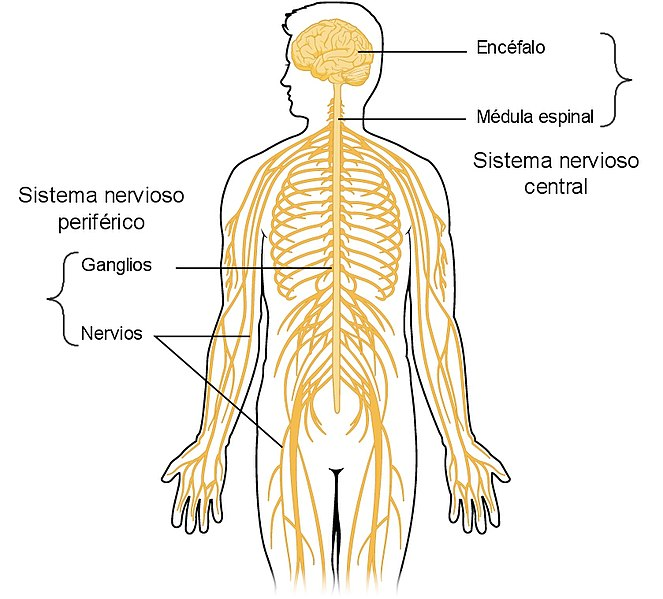
\includegraphics[scale=0.5]{../Figuras/Nervous_System.jpg}
 \caption{Sistema nervioso periférico y central.  \textit{Overview of Nervous System esp, OpenStax, 20 diciembre 2018, WIKIMEDIA COMMONS, \url{https://upload.wikimedia.org/wikipedia/commons/0/07/1201_Overview_of_Nervous_System_esp.jpg}, CC BY-SA 4.0}}
 \label{fig:SNCySNP}
\end{figure}


En el sistema nervioso periférico tenemos al:


\begin{itemize}
 \item \textbf{Sistema somático} se controla de forma voluntaria, se conforma de nervios conectados a músculos voluntarios esqueléticos y receptores sensoriales, de los cuales unos son:
 \begin{itemize}
  \item de entrada, \textbf{aferentes}.
  \item de salida, \textbf{eferentes}.
 \end{itemize}


 \begin{figure}[h]
 \centering
 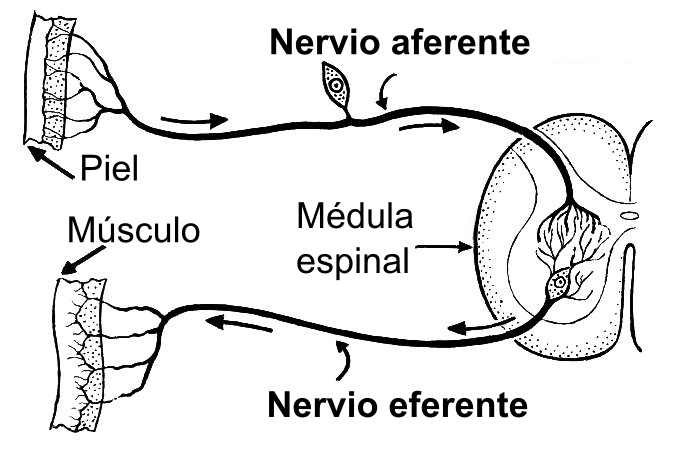
\includegraphics[scale=0.5]{../Figuras/afferent_efferent.png}
 \caption{Diagrama explicativo del recorrido eferente y el aferente.  \textit{Pearson Scott Foresman, 26 August 2010, WIKIMEDIA COMMONS, \url{https://upload.wikimedia.org/wikipedia/commons/3/3e/Afferent_\%28PSF\%29.es.png}, CC0}}  \textcolor{red}{¿Fref?}
 \label{axonesSA}
 \end{figure} 
 
\item \textbf{Sistema autónomo} funciona de forma involuntaria, se conforma de nervios que se conectan con el corazón, los vasos sanguíneos, los pulmones, el estómago, los intestinos, glándulas.
\end{itemize}


Ahora respecto al sistema nervioso central, lo integran:


\begin{itemize}
 \item La médula espinal
    \begin{itemize}
     \item Dentro de esta hay una organización, nuestro sistema va a procesar la información en capas.  Sin embargo, aquí también encontramos \textbf{ciclos de retroalimentación local}, es decir, nervios que no necesitan pasar por todo el procesamiento cerebral, las señales que entran simplemente llegan a una fase local de procesamiento e inmediatamente reaccionan (ver el ejemplo de la \fref{actReflejo}). Los \emph{reflejos} ocurren en un ciclo local y esto también puede convertirse en algo muy importante a la hora de hacer cómputos, no siempre es necesario pasar todo por todas las capas de procesamiento. 


     \begin{figure}[h]
      \centering
      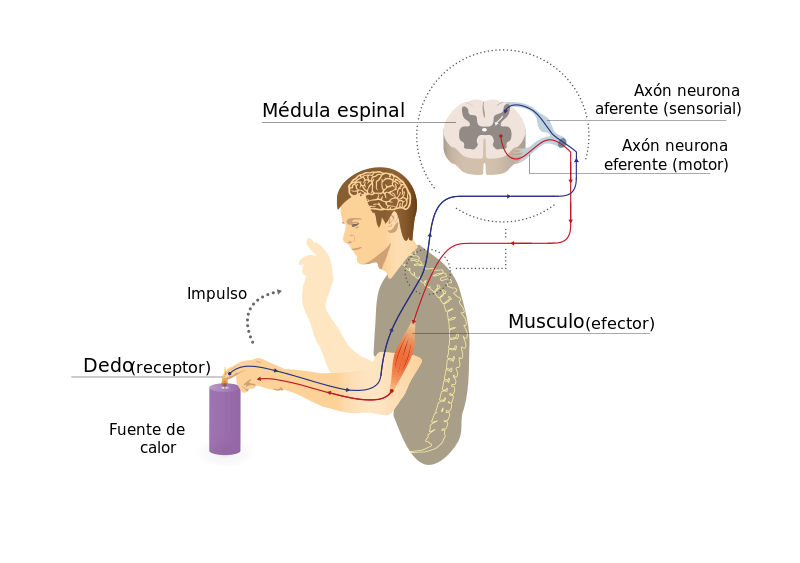
\includegraphics[scale=0.4]{../Figuras/actReflejo.png}
      \caption{ Esquema explicativo del arco reflejo.  \textit{Marta Aguayo, 18 diciembre 2014, WIKIMEDIA COMMONS, \url{https://upload.wikimedia.org/wikipedia/commons/c/cb/Imgnotraçat_arc_refelx_esp.svg}, CC BY-SA 3.0.}}
      \label{actReflejo}
     \end{figure}


     \item \textbf{Señales de control motor descendientes} del cerebro hacia las neuronas motoras, estas son señales que provienen de un campo en una capa mucho más alta de procesamiento y provocan movimientos.
     
     \item \textbf{Axones sensoriales ascendentes} donde el cuerpo de la neurona está afuera \textcolor{red}{¿afuera de dónde?} y la información va a viajar hacia arriba, desde los músculos, piel y  estas señales viajan hasta el cerebro.  


     \end{itemize}


 \item El encéfalo
\end{itemize}


 En su mayoría, cada colección de nervios que sale de la base del cerebro se asocian con funciones muy específicas.
 
 Notas:
 
 \begin{itemize}
  \item El sistema nervioso está compuesto por diferentes niveles locales, entradas y salidas.
  
  \item El procesamiento que esté ocurriendo en el encéfalo puede realizarse a través de diferentes capas y eso se verá reflejado cuando nosotros definamos arquitecturas para las redes neuronales.
  
  \item Las redes neuronales actuales, que han tenido más éxito, se componen de diferentes subunidades o diferentes redes realizan cómputos locales. Es decir esta estructura global que estamos viendo,  se está empezando a reproducir/imitar ya con las redes neuronales computacionales.


 \end{itemize}




\subsection{Cerebro}


En esta parte vamos a preocuparnos sobre todo por la parte funcional. Haciendo una breve analogía, vamos a hacer una visión general del ``\textit{hardware}'', para ver qué efectos va a tener en el ``\textit{software}''.
La arquitectura de cada cerebro es diferente al cerebro de otras personas, aunque por lo general comparten divisiones en grandes regiones bien identificadas. Se ha intentado averiguar qué está haciendo cada región con diferentes estudios.  Por ejemplo: se recurre a detectar cuánta sangre se está bombeando en diferentes regiones del cerebro dependiendo de los estímulos que se le presentan a una persona; o si alguna persona tiene un padecimiento se toman escaneos para ver qué regiones del cerebro están funcionando y cuáles presentan lesiones, a partir de las lesiones y de la identificación de la actividad que ya no se puede realizar de forma normal, se infiere qué región era responsable de esa actividad, que ahora está dañada.


Gracias a esos estudios, se ha logrado identificar más o menos en manera general, a qué se dedica cada una de las regiones del cerebro. En ocasiones no se puede decir exactamente qué tan vinculadas están las regiones o por qué se están activando otras regiones.  Hay partes funcionales que se comparten entre las diferentes regiones y no están ubicadas en un solo lugar. 


Otra parte importante a mencionar es el cerebelo, que se considera prácticamente vital, es responsable de funciones tales como el equilibrio, la coordinación, el control fino de los músculos, de hecho tiene más neuronas que el cerebro y aun así hay niños que nacen y viven sin cerebelo. 




A continuación se mencionan algunas de las diferentes funciones de las regiones, que se han identificado en la \fref{cerebro}: 


 \begin{figure}[h]
  \centering
  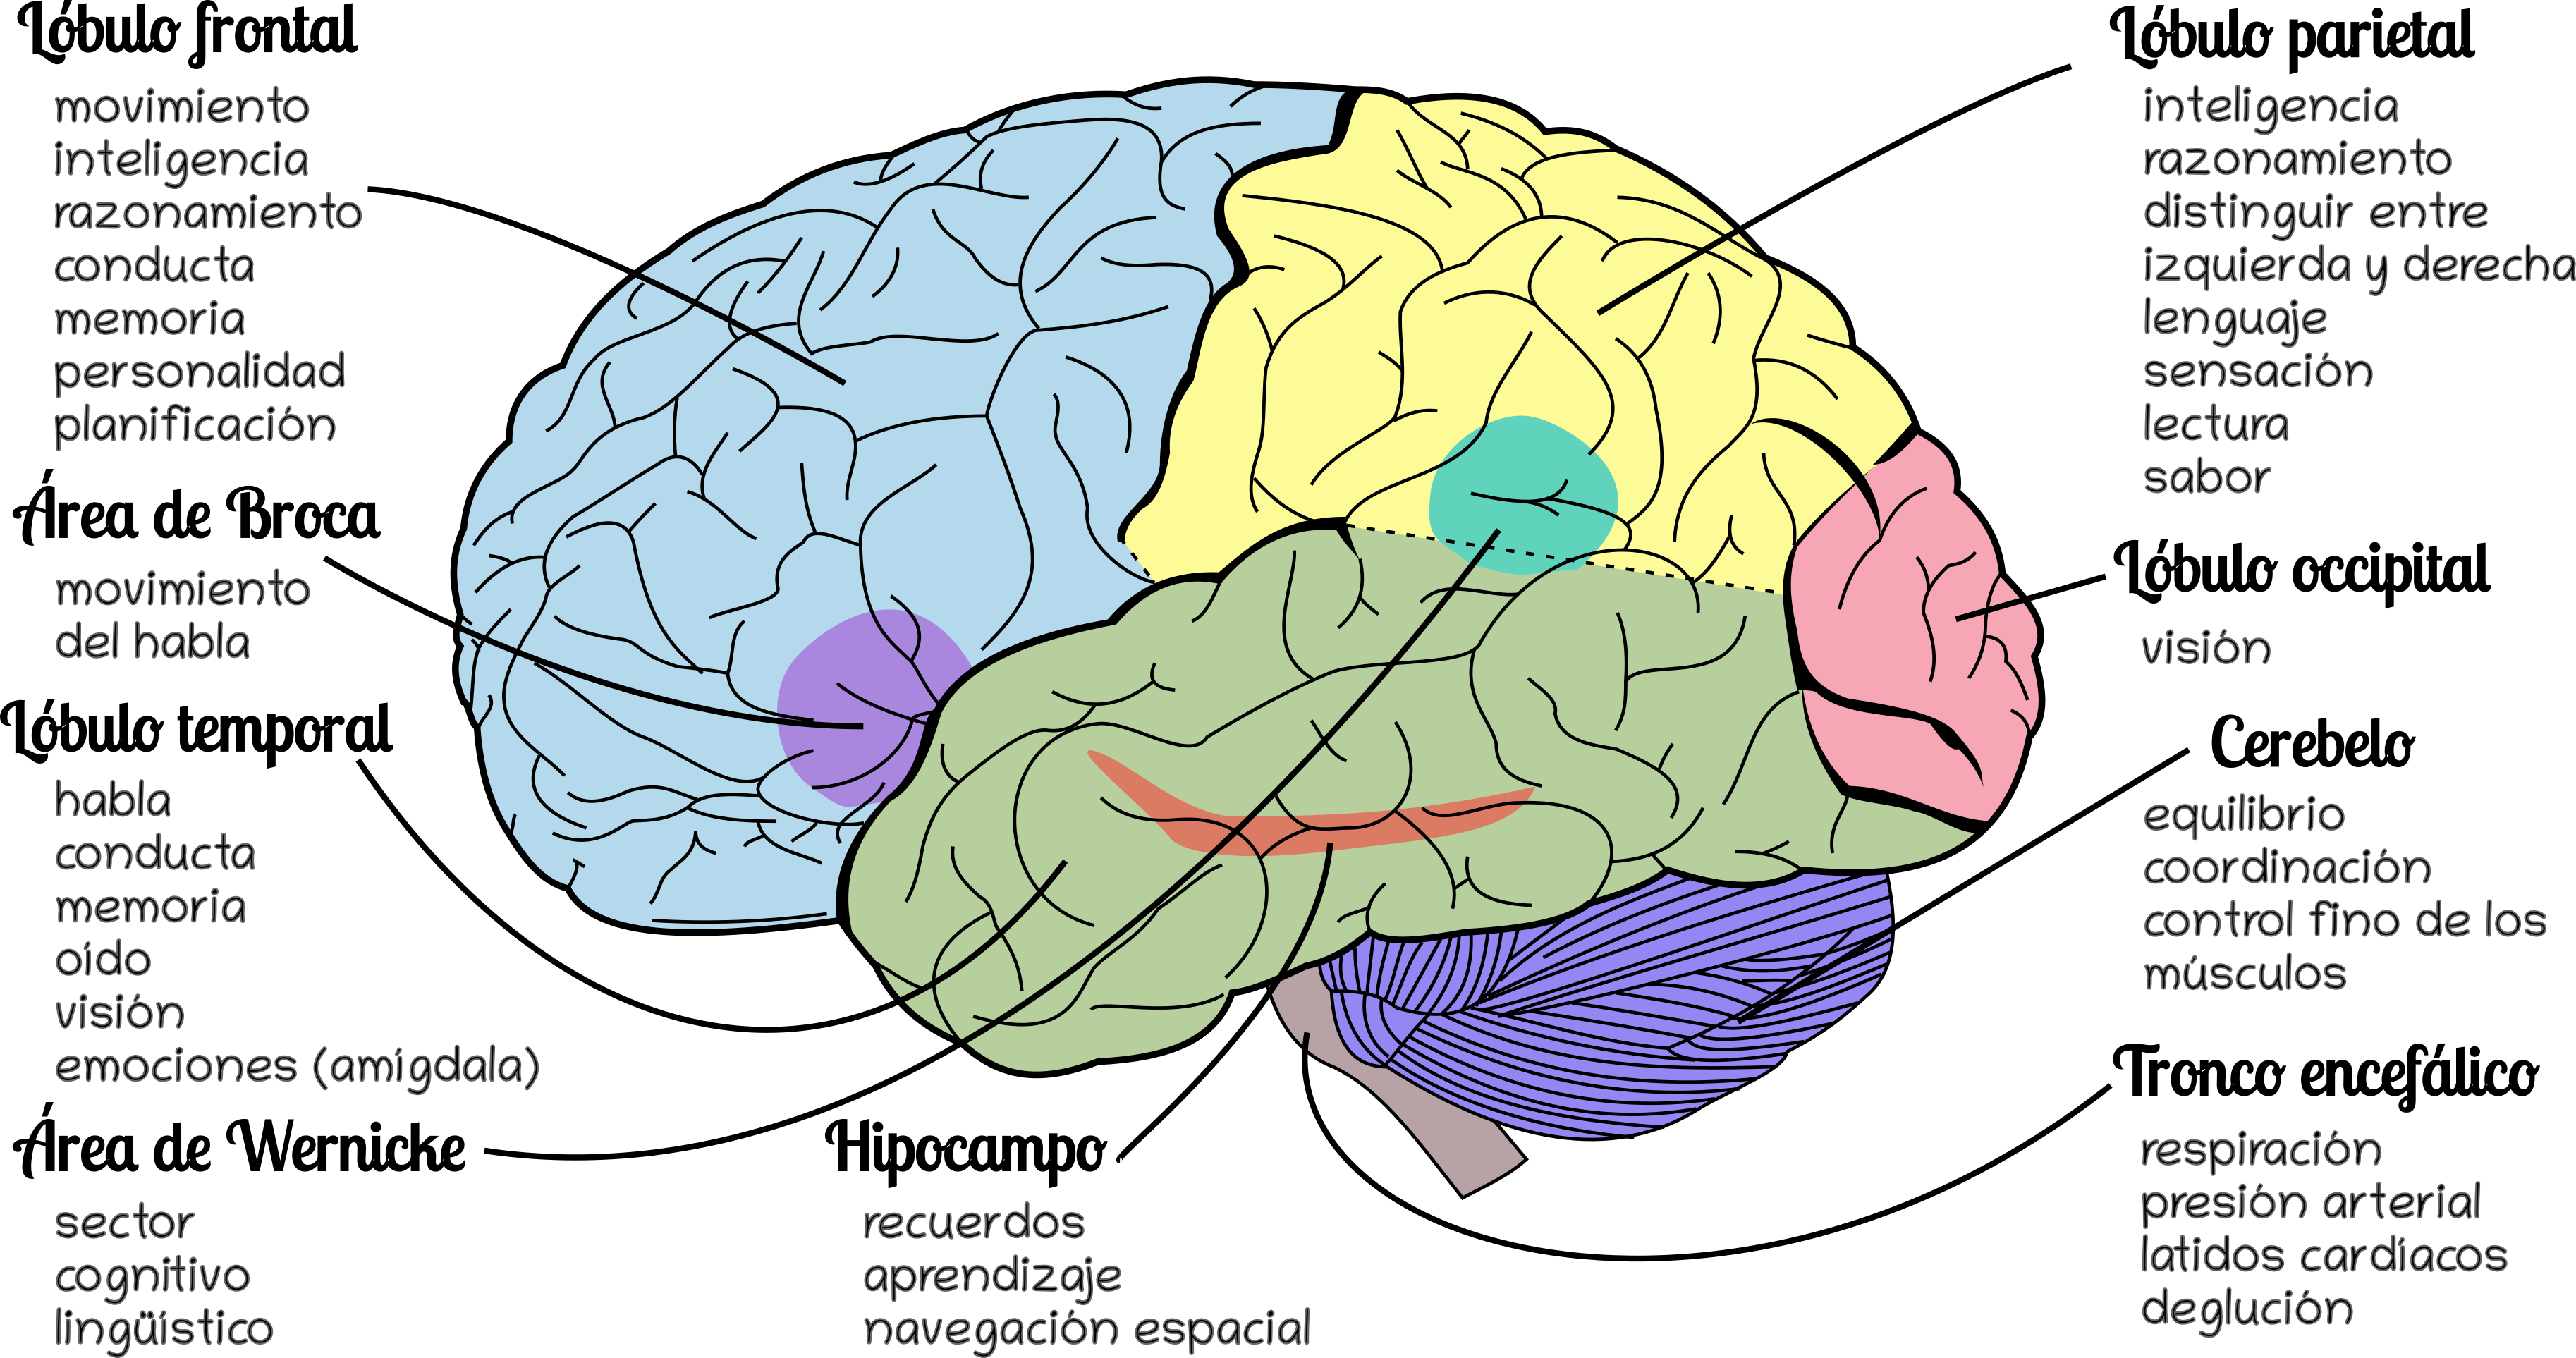
\includegraphics[width=0.9\textwidth]{../Figuras/cerebro.png}
  %Presentación Sistema Nervioso
  \caption{Diagrama básico de las regiones del cerebro.}\label{cerebro}
 \end{figure}


\begin{description}
 \item \textbf{Lóbulo frontal} se le puede asociar con la parte del raciocinio,  la parte de inteligencia, la conducta, la memoria, la personalidad, la capacidad para realizar planes complejos a largo plazo y también es responsable de algunas actividades de movimiento. Dentro de este destaca el Área de Broca, su principal función es el movimiento del habla, mover los labios, la boca.
 
 \item \textbf{Lóbulo temporal} aquí está otra parte del habla, que tiene que ver más con el uso de símbolos para el lenguaje, la conducta, memoria, aquí se procesan las señales provenientes del oído, un poco de visión y emociones. Dentro de este está (compartida con el lóbulo parietal) el área de Wernicke, que trabaja con la parte lingüística y de cognición.
 
 \item \textbf{Hipocampo}, se encuentra en la base del cerebro. Trabaja con recuerdos, aprendizaje y navegación espacial, cómo sabemos cómo llegar de un lado hacia otro.
 
 \item \textbf{Lóbulo parietal} trabaja con la inteligencia, razonamiento, distinguir entre izquierda y derecha, lenguaje, sensación, lectura y sabor. 
 
 \item \textbf{Lóbulo occipital} se dedica prácticamente solamente a visión, es una región un tanto amplia. En particular en el área de robótica cuando están programando un robot móvil, los robots tienen dos laptops y una de ellas se dedica prácticamente sólo a procesar la visión.
 
 \item \textbf{Cerebelo} se encarga del equilibrio, la coordinación fina de los músculos.
 
 \item \textbf{Tronco encefálico} se encarga de la respiración, presión arterial, latidos cardíacos, deglución, conciencia.
\end{description}


\subsection{Zonas funcionales}
Para visualizar mejor la parte de la arquitectura que tiene el cerebro para realizar todo lo que se le conoce como ``la ruta desde la sensación hasta la cognición'' veremos un diagrama de la parte funcional del cerebro.  


 \begin{figure}[h]
  \centering
  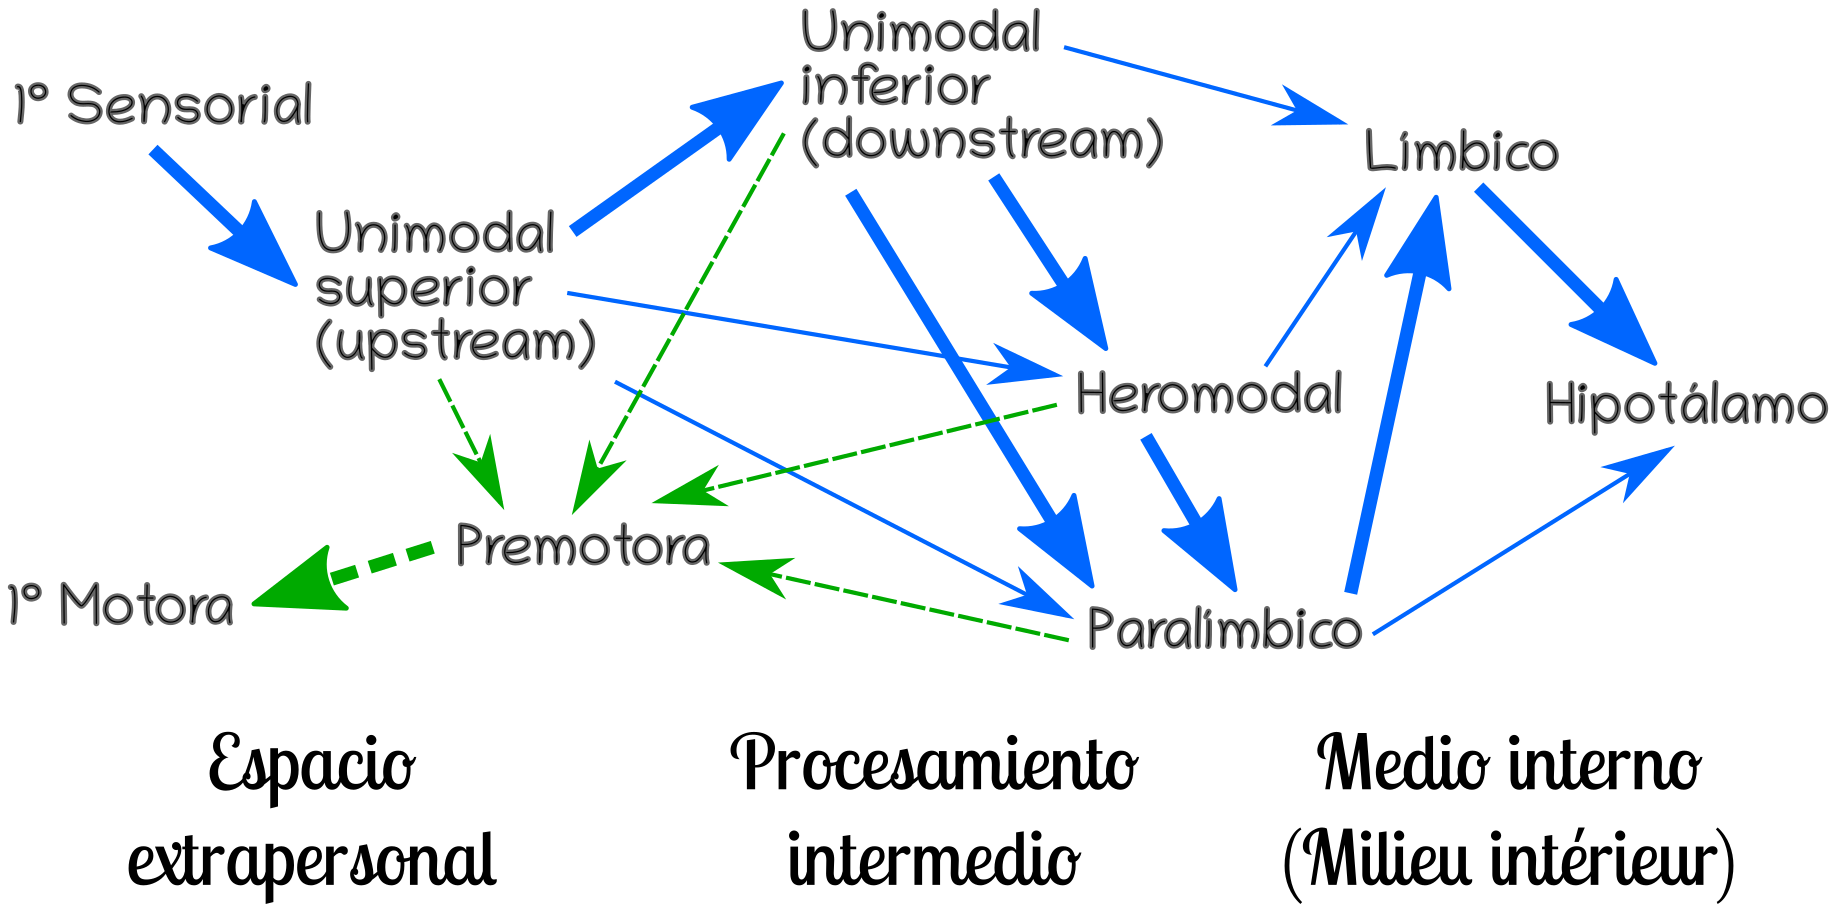
\includegraphics[width=0.9\textwidth]{../Figuras/zonasFuncionales.png}
  %Presentación Sistema Nervioso (11)
  \caption{Diagrama de la arquitectura del cerebro a nivel funcional. \parencite{Mesulam1998}}
  \label{fig:zonasFun}
 \end{figure}


Explicando la \fref{fig:zonasFun}, en la primera parte (espacio extrapersonal) vamos a pensar en la entrada sensorial, que se enfoca muchísimo en la parte de visión y audio (en general todos los sentidos), notamos que de las neuronas que están en la parte sensorial, su primera conexión es hacia una capa que se le llama unimodal superior,  aquí se procesa la información de cada sentido de manera individual, es decir, las neuronas o solamente están procesando visión o solamente audio, todavía no se mezclan, por ejemplo de visión, se separan colores e intensidad lumínica, se empieza a detectar algunas esquinas, alguna inclinación, la dirección de las luces y las sombras. Notemos que desde aquí hay una rápida conexión a la sección premotora y luego hacia la parte motora, recordando la mención de los circuitos locales y de reflejos, aquí prácticamente lo podemos ver en este pequeño camino.


Pasando de este primer procesamiento básico entramos al siguiente que es el unimodal inferior.  Aquí aún se está trabajando con procesamiento de una sola modalidad: visión sigue siendo visión, audio sigue siendo audio; pero ya son procesamientos un poco más complejos, por ejemplo, reconocimiento de rostros, de objetos. En esta parte tenemos un rápido ciclo de regreso a la parte premotora, por ejemplo la acción de ver a mi mamá y saludarla (aquí aún no se tiene que razonar demasiado). 


La siguiente fase (medio interno), comprende tres áreas.  En el área \textbf{heromodal} ya se integran diferentes modalidades, como audio y visión; por ejemplo: oigo que me hablan y volteo a ver, aquí se está juntando ambas cosas.  El \textbf{límbico} y el \textbf{paralímbico} trabajan con la parte de las emociones y conceptos abstractos.


Finalmente, llegamos al \textbf{hipotálamo}, que es donde están todas las emociones, en las conexiones entre estas regiones estarían los procesamientos de alto nivel.


Ahora estas diferentes regiones se replican de cierta manera cuando estamos haciendo los diseños de las arquitecturas modernas para redes neuronales.
En algunas ocasiones se comienza con algunas capas de neuronas, haciendo procesamientos con una sola modalidad, extrayendo datos básicos, después se van
componiendo en figuras más complejas y después hasta podemos combinar bloques de neuronas, para poder resolver problemas que tomen en cuenta diferentes modalidades.






 
\section{Neurona biológica}
\subsection{La neurona}

La neurona es un tipo de célula perteneciente al sistema nervioso central, que se comunica tanto por señales eléctricas como por señales químicas. Cada neurona tiene \parencite{sistemaNervioso}:%pag34


 \begin{itemize}
	\item Un cuerpo celular llamado \textbf{soma} que contiene un núcleo y otros componentes celulares.
	\item Una zona de recepción con protuberancias elongadas llamadas \textbf{dendritas}.
	\item Una zona de emisión llamado \textbf{axón}, el cual está compuesto de:
		\begin {itemize}
			\item Cono axónico.
			\item Membrana plasmática axónica y citoplasma.
			\item Recubrimientos de mielina, interrumpido a intervalos regulares por nodos de Ranvier.
			\item Terminales del axón donde se encuentran los botones sinápticos. 
		\end{itemize}
 \end{itemize}


\begin{figure}[h]
 \centering
 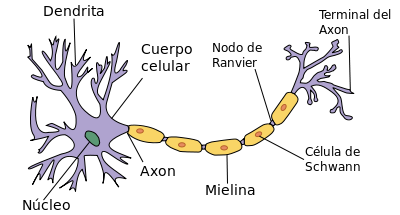
\includegraphics[scale=0.6]{../Figuras/neuronaPartes.png}
 \caption{Neurona, Acracia, 14 January 2007, Wikimedia Commons, \url{https://commons.wikimedia.org/wiki/File:Neurona.svg}, Creative Commons Attribution-ShareAlike 2.5 Generic}
 \label{fig:neuronaP}
\end{figure}

\subsection{Elementos de las neuronas en la transmisión de señales}

Los principales elementos que participan durante la transmisión de señales entre neuronas son \parencite{sistemaNervioso}:


\begin{itemize}
\item \textbf{Impulsos eléctricos:} potenciales de acción, cambios de voltaje que ocurren a lo largo del axón. % Sucede una vez que se acumularon demasiadas señales a través de las dendritas, entonces la neurona puede disparar un impulso eléctrico, a través del axón, que va a provocar que su terminal libere más químicos, estos químicos son los que hacen los efectos pequeños en cada uno de los cuerpos de las neuronas postsinápticas.
Pueden generar dos efectos en la membrana de la neurona: 
	\begin{itemize}
	\item \textbf{El efecto excitatorio}, despolariza la membrana postsináptica. La neurona es más propensa a mandar un pulso eléctrico.  
	\item \textbf{El efecto inhibitorio}, hiperpolariza la membrana postsináptica. La neurona no manda pulso eléctrico.

	\end{itemize}

\item \textbf{Neurotransmisor/es:} donde se encuentra la sustancia química, %\parencite{sistemaNervioso pag.50.}
son los mensajeros químicos que se comunican entre neuronas adyacentes. La liberación de neurotransmisores de una neurona ayudará a despolarizar o hiperpolarizar (aumentar la magnitud de la carga) de la neurona adyacente, lo que hará que sea más o menos probable que ocurra un potencial de acción en la siguiente neurona.
 
\item \textbf{Plasticidad:} La modificación a largo plazo de las conexiones entre neuronas. %Las neuronas cambian, pirden o forman conexiones que permiten el intercambio de nuevos transmisores sin impulsos eléctricos).
\end{itemize}



En el contexto de la transmisión neuronal de señales, es necesario realizar ciertas distinciones para denotar claramente si una neurona particular está recibiendo o transmitiendo una señal. Las distinciones son las siguientes:
 \begin{itemize}
  \item Neurona presináptica: Transmite una señal a otras neuronas o células a lo largo del sistema nervioso.
  \item Neurona postsináptica: Recibe una señal de otras neuronas o células, procesando y respondiendo a dicha señal.
 \end{itemize}  

La transmisión de señales y almacenamiento de información en las neuronas se da de la siguiente forma:\parencite{neurona_A_cerebro}

\begin{enumerate}
 \item La neurona desde sus dendritas recibe señales de otras neuronas vecinas.
 \item Cada señal se va acumulando en su cuerpo hasta el cono axónico, donde se van a estar sumando la contribución de todos los efectos de cambios de potencial.
 \item En el momento que se rebase un cierto valor umbral, la diferencia de potencial se propaga hasta los botones terminales.
 \item La neurona entra en un período refractario, donde empieza a cambiar el potencial entre el cono axónico y el axón de la neurona.
 \item Se transmite un disparo eléctrico en seguida.
 \item La neurona se va a quedar totalmente quieta, durante un breve momento para que la señal pueda viajar hacia el axón.
 \item Se va a notar un cambio muy violento en el voltaje, que se va recorriendo a lo largo de todo el axón. 
\end{enumerate}

A lo anterior también se le conoce como neurotransmición que esta  descrita con mayor precisión en la figura  \fref{fig:nTransmision}.

\begin{figure}[h]
 \centering
 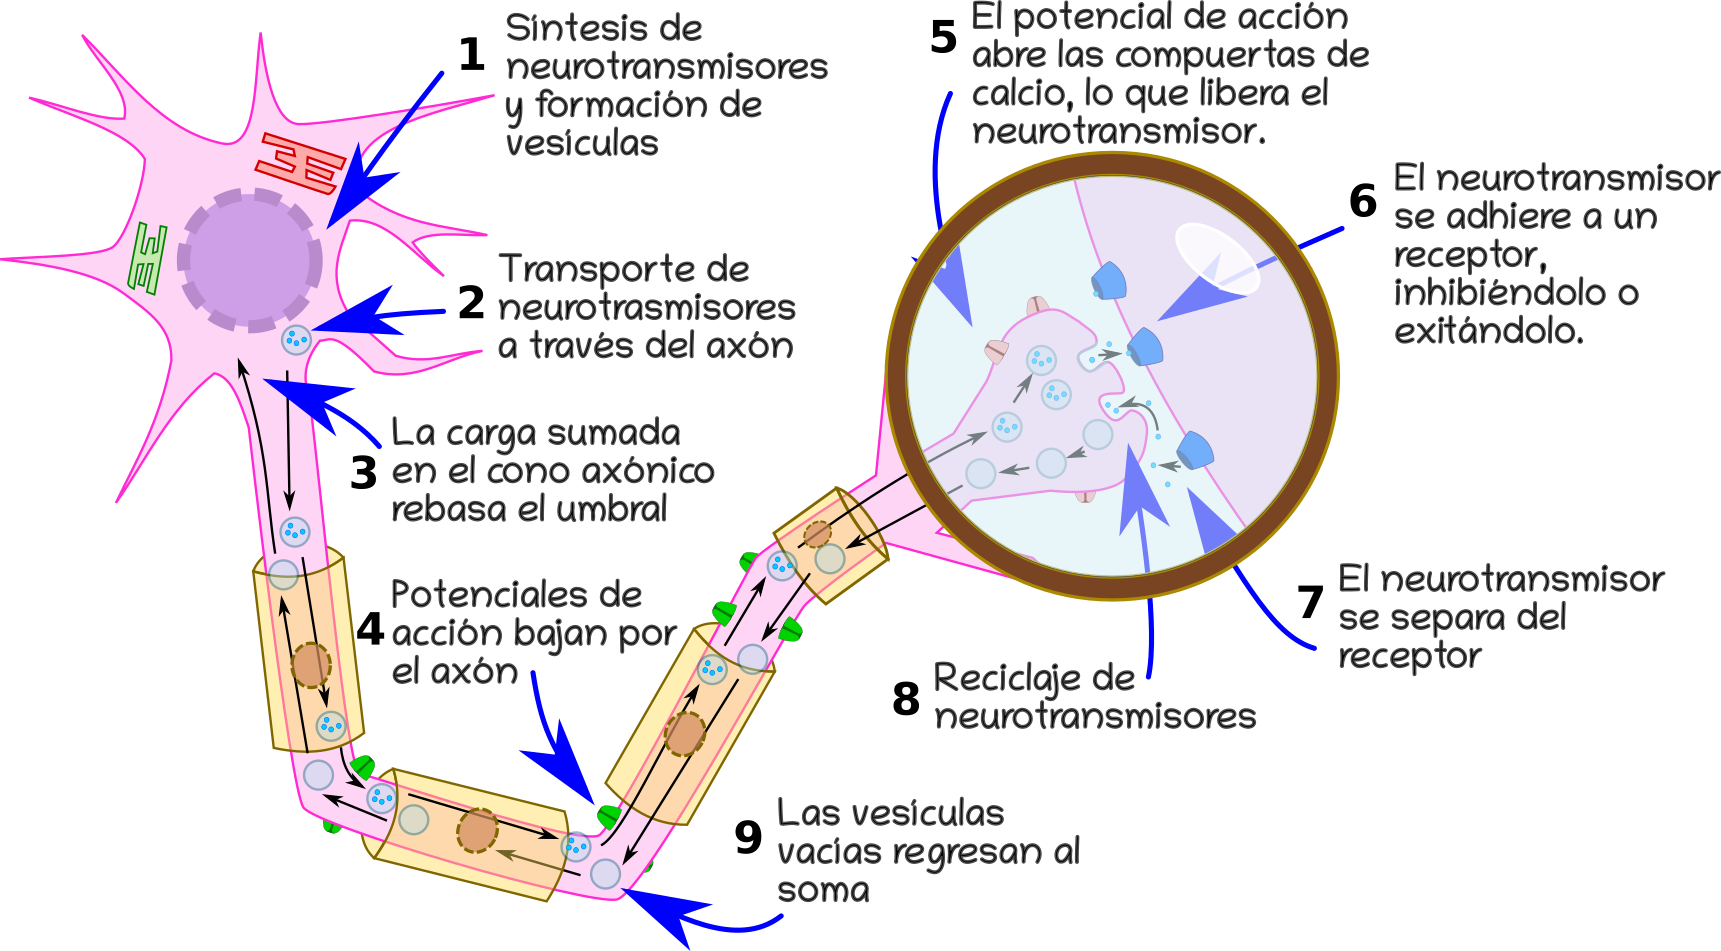
\includegraphics[scale=0.2]{../Figuras/neurotransmision.png} 
 \caption{Esquema detallado de una neurotransmisión. Author: Verónica Arriola Rios.}
 \label{fig:nTransmision}
\end{figure}


La neurona a lo largo de su axón, está cubierta de nodos (y de células de mielina). Estos nodos están para evitar que se distorsione o se pierda la señal recibida en la dendritas, en ellos se recarga la señal para que llegue desde el soma hasta las terminales del axón. Y así pase a la neurona postsináptica, que a su vez la pasará a otra hasta lograr llegar a algun nervio del SNP. 


\subsection{Sinapsis}

 El espacio donde dos neuronas en estrecha proximidad, se transmiten información se llama \textbf{sinapsis}. La sinapsis (típica) se establece entre el axón de una neurona y la dendrita de otra neurona. \parencite{sistemaNervioso}%pag50.



\begin{figure}[h]
 \centering
 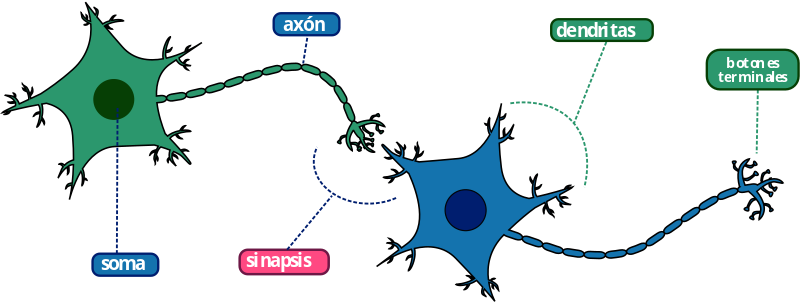
\includegraphics[scale=0.5]{../Figuras/Part_of_neurons_in_Spanish.png}
 \caption{Part of neurons in Spanish, Dana Scarinci Zabaleta, 24 February 2019, Wikimedia Commons, \url{https://commons.wikimedia.org/wiki/File:Part_of_neurons_in_Spanish.svg}, OpenStax, CC0}
 \label{fig:sinapsisN}
\end{figure}


\subsubsection{Clasificación de sinapsis}

Los dos tipos de sinapsis (relevantes para el curso) son:

\begin{description}
 \item [Sinapsis eléctrica:] las membranas de las células pre y post sinápticas se unen en la brecha sináptica, que son pequeños canales que permiten el paso de iones (\fref{fig:sinapsisN}).


\begin{figure}[h]
 \centering
 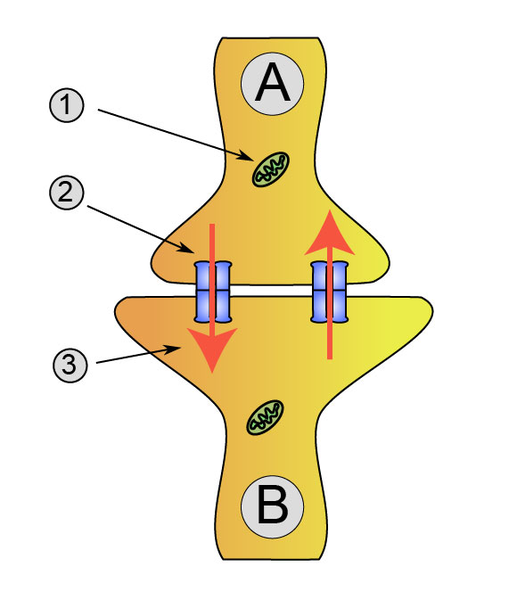
\includegraphics[scale=0.2]{../Figuras/sinapsisElectrica.png}
 \caption{Synaptical transmission (electrical). Neurona A transmisora, Neurona B receptora, 1. Mitocondria, 2. Uniones gap formadas por conexiones, 3. Señal eléctrica, Nrets~commonswiki, 23 September 2005, Wikimedia Commons, \url{https://commons.wikimedia.org/wiki/File:Synapse_diag2.png}, Inkscape 0.42, CC-BY-SA 3.0}
 \label{fig:sinapsisN}
\end{figure}
 
 \item [Sinapsis química:] la neurona libera moléculas neurotransmisoras a otra neurona adyacente en un pequeño espacio, la brecha sináptica (\fref{fig:sinapsisQ}).


\begin{figure}[h]
 \centering
 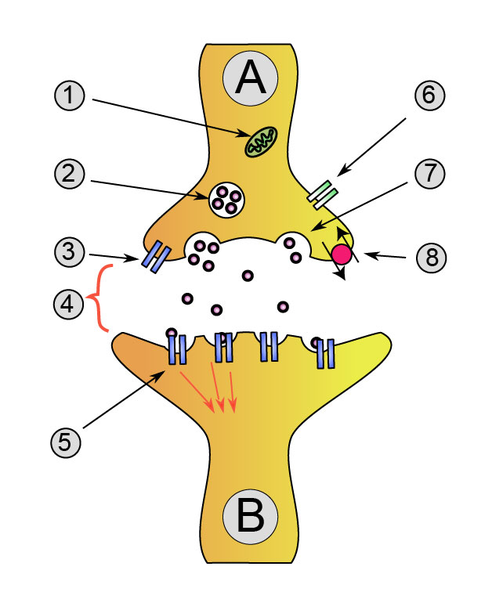
\includegraphics[scale=0.2]{../Figuras/SinapsisQuimica1.png}
 \caption{Synaptical transmission (chemical). Neurona A transmisora, Neurona B receptora, 1. Mitocondria, 2. Vesícula sináptica llena de neurotransmisor, 3. Autorreceptor, 4. Brecha sináptica, 5. Receptor de neurotransmisores, 6. Canal de calcio, 7. Neurotransmisor liberador de vesículas fusionadas, 8. Bomba de recaptación de neurotransmisores, Utilisateur:Dake, 23 September 2005, Wikimedia Commons, \url{https://commons.wikimedia.org/wiki/File:Synapse_diag1.png}, Inkscape 0.42, CC-BY-SA 3.0}
 \label{fig:sinapsisQ}
\end{figure}

\end{description}








\subsection{Señal eléctrica}

El paso de las señales eléctricas entre neuronas, se da gracias a los canales de iones. Los que destacan son los siguientes:

\begin{itemize}
\item \textbf{Canal por fuga:} Estos se abren y cierran aleatoriamente, todo el tiempo están activos en la neurona. Por ejemplo: sodio y potasio.

\item \textbf{Canal regulado por ligado:} En este un neurotransmisor que es el que provoca o impide que se abran. 

\item  \textbf{Canal por estímulo mecánico:} Permiten que pasen más iones o menos iones dependiendo si se ejerció una presión, por ejemplo, con las neuronas cerca de la piel.
\item \textbf{Canales regulados por el voltaje:} Un voltaje es el que abre o cierra el canal. Permite o no el paso del pulso eléctrico. % Existen una variante de este tipo, el cual tiene una pequeña compuerta abajo, que la puede cerrar independientemente.
\end{itemize}


Existen realmente una buena cantidad de iones presentes en el cerebro, pero los más protagónicos son \textbf{potasio}, el \textbf{sodio} y el \textbf{cloro}. Los que vamos a utilizar para un modelo matemático de las neuronas. Veremos más detalles en el siguiente capítulo.


\begin{figure}[h]
 \centering
 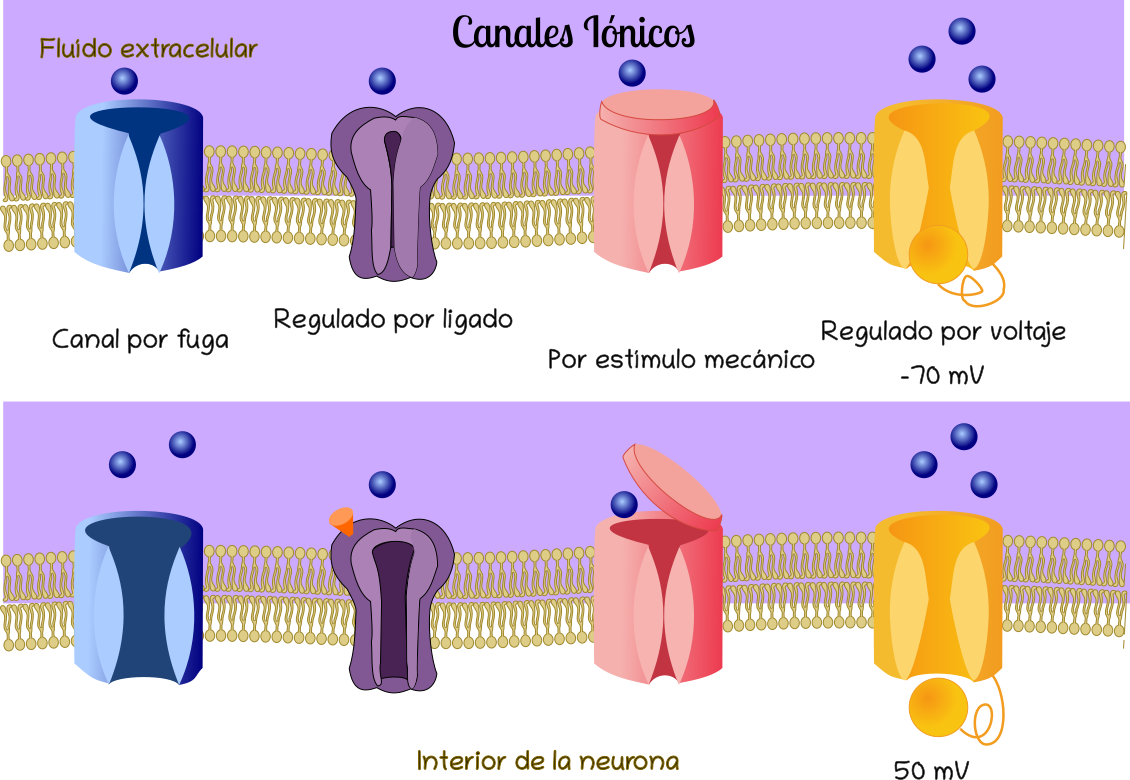
\includegraphics[scale=0.28]{../Figuras/canalesIonicos.png}
 \caption{Representación de la clasificación de los canales iónicos.}
 \label{fig:MembranaP}
\end{figure}



\subsubsection{Neuroplasticidad}

Una característica importante de la conexión entre neuronas es la neuroplasticidad, que es lo que nos permite el aprendizaje a largo plazo en el cerebro, es un mecanismo de aprendizaje del cerebro en el cual cuando las neuronas se activan simultáneamente con frecuencia la conexión entre ellas se fortalece.


Este mecanismo constituye la principal inspiración para el diseño de las redes neuronales artificiales, concretamente en esto se inspiran los algoritmos de entrenamiento. Calculamos, qué conexiones debemos reforzar y cuáles debemos de debilitar para que nuestras redes neuronales calculen las funciones que a nosotros nos interesan. 








\chapter{Modelo de Hodgkin-Huxley}

\section{Introducción}

En esta sección se aborda el proceso de transmisión de información y se analizan las operaciones biológicas que hacen posibles los cómputos en el cerebro. Para empezar a modelar una red neuronal se detallará primero la dinámica de los disparos neuronales.

Recordando los conceptos abordados en el  capítulo  anterior, las neuronas son células especializadas del sistema nervioso central que se comunican mediante señales tanto eléctricas como químicas.  Son células con núcleo, axón y dendritas capaces de transferir impulsos eléctricos. La transmisión de un pulso eléctrico se lleva a cabo desde el soma a través de sus membranas, pasando por los nodos de Ranvier a lo largo del axón, hasta la terminal del axón en los botones sinápticos. Las neuronas hacen sinapsis  permitiendo que el pulso llegue a las dendritas de la neurona postinanáptica, mediante canales iónicos. \parencite{neurona_A_cerebro}

El pulso eléctrico que se desplazo desde el cono axónico de la neurona presináptica hasta la neurona postsináptica, se genera por la diferencia de potencial existente entre el interior y el exterior de la neurona, el cual resulta de las varias concentraciones de iones en ambos lados de la membrana plasmática. Los estados potenciales neuronales presentes en la membrana plasmática del axón se distinguen en los siguientes \parencite{HH}:

\begin{itemize}
\item \textbf{Potencial de reposo:} Se refiere a la diferencia de cargas eléctricas a través de la membrana celular cuando no hay una señal nerviosa en curso. La membrana está polarizada a -70 mV, lo que significa que tiene una carga positiva en el exterior (por la presencia de iones de sodio, Na+) y una carga negativa en el interior debido a iones como el cloruro (Cl-) y proteínas. En este estado, la membrana no transmite señales nerviosas. Ver la figura \fref{fig:MembranaP} lado derecho.

\item \textbf{Potencial de acción o membrana:}  Se produce cuando un estímulo alcanza un nivel umbral de 55 mV. Este evento despolariza la membrana, lo que significa que cambia rápidamente su polaridad de negativa a positiva. Esto ocurre porque se abren canales de iones de sodio (Na+) y potasio (K+), permitiendo el flujo de estos iones a través de la membrana, ver la figura \fref{fig:MembranaP} lado izquierdo. Este cambio rápido en la polaridad de la membrana es lo que impulsa el avance de la señal nerviosa. Las etapas del potencial de acción está representado en la figura \fref{fig:graficaP}
\end{itemize}


\begin{figure}[h]
 \centering
 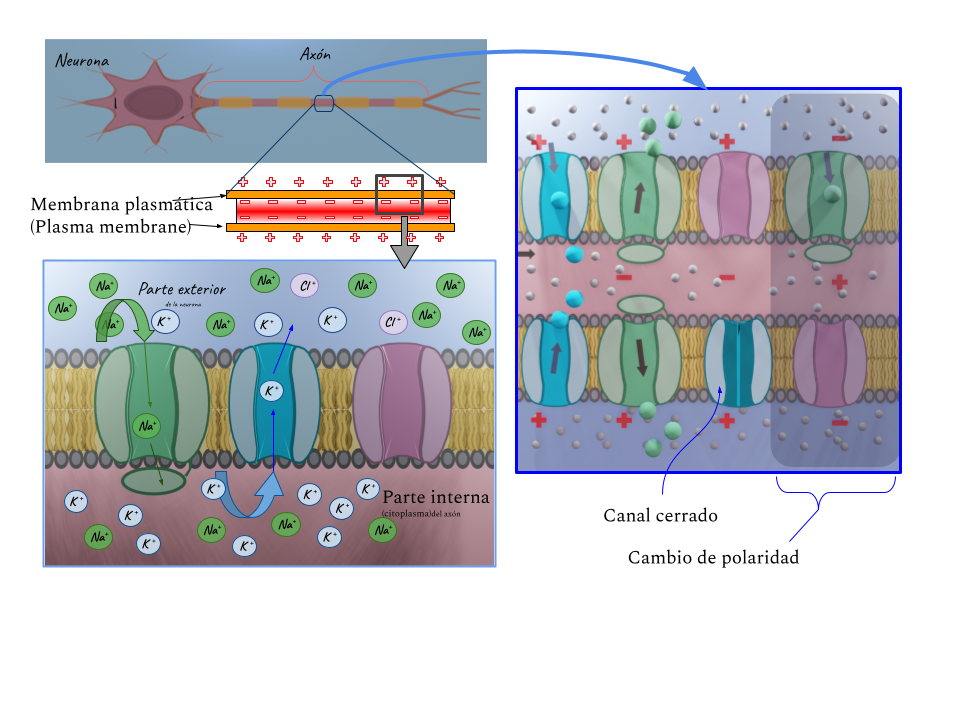
\includegraphics[scale=0.5]{../Figuras/MembranaP.png}
 \caption{Representación de la membrana axónica en potencial de reposo en la parte inferior izquierda, y en la parte derecha con un estímulo que genera el cambio de polaridad en la misma, así como el cierre de canales y paso de iones.}
 \label{fig:MembranaP}
\end{figure}

\begin{figure}[h]
 \centering
 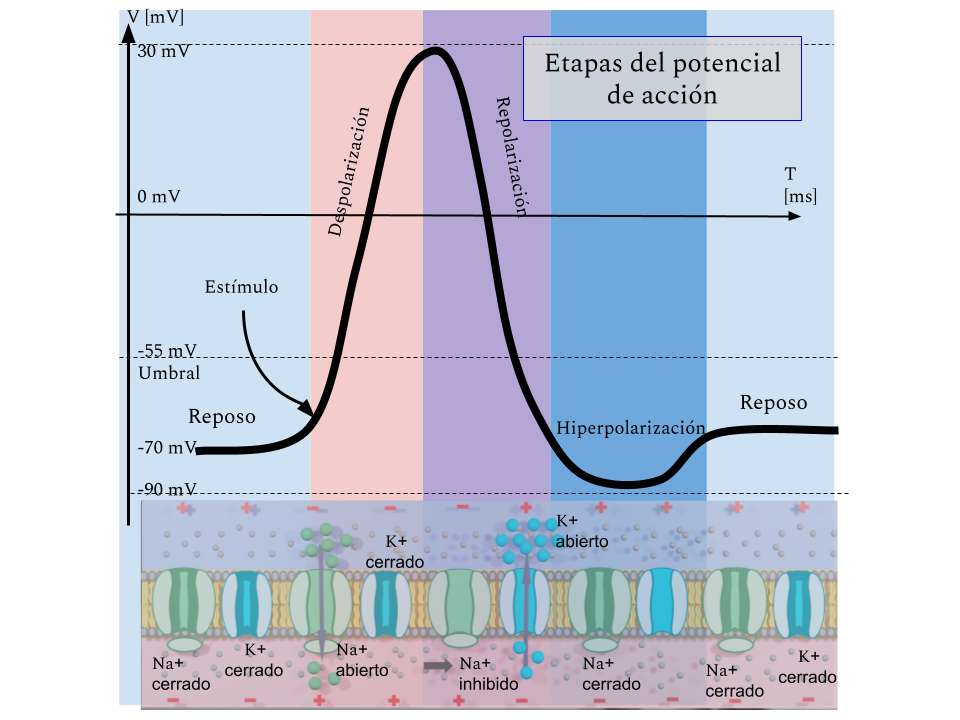
\includegraphics[scale=0.5]{../Figuras/Grafica.png}
 \caption{Representación gráfica de la respuesta de los canales iónicos de sodio (Na+ en verde) y potasio (K+ en azul) ante un estímulo de voltaje, dando como resultado un potencial de acción que viajará a lo largo de todo el axón.}
 \label{fig:graficaP}
\end{figure}

Los pioneros en el estudio del potencial de acción y elaboración de un modelo para la unión sináptica eléctrica fueron Alan Lloyd Hodgkin y Andrew Fielding Huxley alrededor de 1952. Este modelo matemático, intentaba esclarecer los procesos neuronales, surgió a partir de investigaciones experimentales  \footnote{El texto original de este experimento se puede encontrar en la siguiente url: \url{ https://physoc.onlinelibrary.wiley.com/doi/pdf/10.1113/jphysiol.1952.sp004764}}.

Estos científicos llevaron a cabo sus estudios utilizando un calamar gigante, un animal que puede alcanzar hasta 4 metros de longitud y posee un axón a proporción, que se extiende casi a lo largo de la mitad del cuerpo del calamar y tiene un grosor de medio milímetro, en comparación con el tamaño estándar del axón de una neurona, que oscila entre 1 y 20 micrómetros. 
El axón del calamar gigante es tan grande que les permitió introducir dispositivos para medir el voltaje, es decir, la diferencia de potencial entre el interior y exterior de la neurona. Con estas mediciones experimentales, lograron determinar las dinámicas de las cargas eléctricas tanto en el interior como en el exterior de la neurona, lo que facilitó el estudio de la transferencia de electricidad durante la activación de un impulso nervioso.
 

\section{Membrana y canal}

Durante las observaciones del flujo de corrientes eléctricas el sistema parecía comportarse como un circuito eléctrico, donde la membrana actuaba como un componente poroso que \textit{funciona como un capacitor}, almacenando ligeramente las cargas cuando intentan pasar de un lado a otro. Además esta membrana tiene la cualidad de permitir el paso selectivo de iones en ciertos momentos, es decir es una estructura \textit{semipermeable} que se representa con \textit{resistencias variables}. Ver Figura \ref{fig:ModelHh}.

Los canales de iones permiten o bloquean el flujo de iones dependiendo de la diferencia de potencial que exista entre el interior y el exterior de la membrana y de su estado de reposo particular. Por tanto es necesario agregar los potenciales de reposo para cada canal al modelo, en la figura \ref{fig:circuito} se agregan.


\begin{figure}[h]
 \centering
 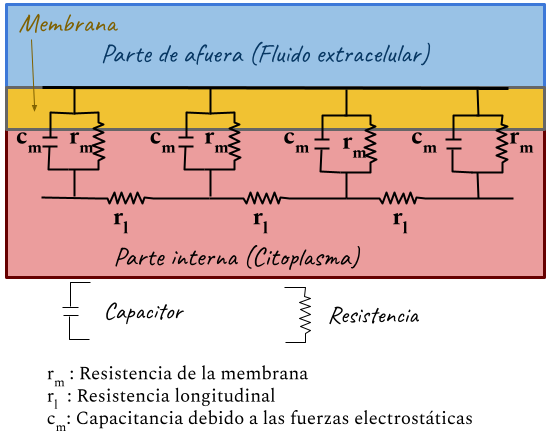
\includegraphics[scale=0.5]{../Figuras/ModeloHH.2}
 \caption{Un primer modelo de la membrana axónica modelada como circuito eléctrico.}
 \label{fig:ModelHh}
\end{figure}



\begin{figure}[h]
 \centering
 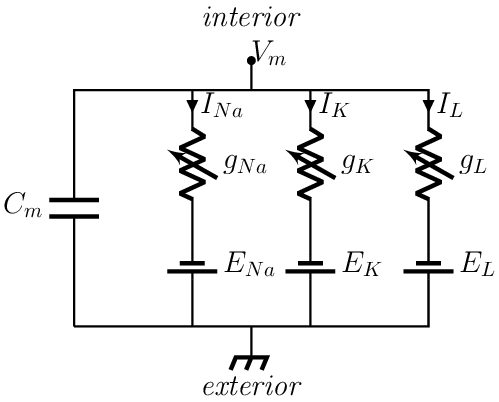
\includegraphics[scale=0.5]{../Figuras/circuito.png}
 \caption{Modelo de la membrana axónica modelada como circuito eléctrico, con los distintos canales presentes y sus voltajes en reposo.}
 \label{fig:circuito}
\end{figure}

Los elementos necesarios para el modelo de la membrana son los siguientes:
\begin{itemize}
\item Potenciales eléctricos \emph{E ó  V}; Se mide en \emph{mV}.
    \begin{itemize}
     \item \emph{E\textsubscript{(Na,K,L)}} 
     Potencial de equilibrio o reposo para los iones de sodio (Na), potasio (K) y cloruro y de fuga (L). 
     \begin{itemize}
        \item E \textsubscript{Na}  \emph{50mV}
        \item E \textsubscript{Ca}  \emph{150mV}
        \item E \textsubscript{K}   \emph{- 80mV}
        \item E \textsubscript{Cl}  \emph{- 60mV}
        \end{itemize}

     \item \emph{V\textsubscript{m}} Potencial eléctrico de la membrana. 
     \end{itemize}

\item Corriente \emph{I}; Movimiento de cargas. Se mide en \emph{µA}.
    \begin{itemize}
     \item \emph{I\textsubscript{(Na,K,L)}} corriente entrante a los canales de Na, K o L.
     \end{itemize}

\item Resistencia \emph{R}; Medida de la oposición al movimiento de las partículas cargadas.
\item Capacitancia o capacidad eléctrica \emph{C} . Cantidad de energía eléctrica almacenada en un capacitor para una diferencia de potencial eléctrico dada.
    \begin{itemize}
     \item \emph{C\textsubscript{m}} la capacitancia de la membrana. 
     \end{itemize}

\item Conductancia \emph{g}; Inverso de la resistencia \( \dfrac{1}{R} \) , es decir, facilidad de transmisión de las partículas cargadas.
    \begin{itemize}
     \item \emph{g\textsubscript{(Na,K,L)}}  la conductancia del canal de sodio, potasio, cloro y fuga. 
     \end{itemize}

\end{itemize}

\section{Modelo de los canales de inoes}

En la figura \fref{fig:MembranaP} se puede ver la representación de membrana y sus lipidos, la carga es almacenada en la membrana por un breve periodo de tiempo, dando como resultado que la bicapa se comporte como un \textbf{capacitor}. Esta membrana también está con cierta resistencia al paso de corriente representado en el diagrama \ref{fig:circuito} \footnote{Otra explicación más detallada la podemos encontrar en \url{https://neurowiki.case.edu/wiki/Action_Potential_IV:_Hodgkin-Huxley_Equations_and_Other_Conductances}} 

La membrana de una neurona es modelada como un elemento de un circuito con capacitancia \emph{C\textsubscript{m}} y potencial \emph{V}, las corrientes que fluye a través de la bicapa lipídica están regidos por las siguientes ecuaciones:

\begin{equation}
  I_{m} = C_{m} \dfrac{dV_{m}}{dt}
  \label{eq:corrientesEnLaMembrana}
\end{equation}


\begin{equation}
  C_{m} \dfrac{dV_{m}}{dt} =  - g_{Na} m^3 h(V - E_{Na} ) - g_{K} n^4 (V - E_{K} ) - g_{L} (V - E_{L} ) + I_ext
  \label{eq:corrientesEnLaMembrana2}
\end{equation}

\begin{equation}
  \dfrac{1}{\gamma(T)}\dfrac{dn}{dt} =  \alpha_{n^\infty} (V)(1 - n) - \beta_{n} (V) n = \dfrac{n(V)-n(t)}{\tau_{n}(V)}
  \label{eq:corrientesEnLaMembrana3}
\end{equation}

\begin{equation}
  \dfrac{1}{\gamma(T)}\dfrac{dm}{dt} =  \alpha_{m} (V)(1 - m) - \beta_{m} (V) m = \dfrac{m^\infty(V)-m(t)}{\tau_{m}(V)}
  \label{eq:corrientesEnLaMembrana4}
\end{equation}

\begin{equation}
  \dfrac{1}{\gamma(T)}\dfrac{dh}{dt} =  \alpha_{h} (V)(1 - h) - \beta_{h} (V) h = \dfrac{h^\infty(V)-h(t)}{\tau_{h}(V)}
  \label{eq:corrientesEnLaMembrana5}
\end{equation}

La ecuación principal es \ref{eq:corrientesEnLaMembrana} que donde la corriente de la membrana está dada por su capacitancia con el cambio voltaje en la membrana respecto al tiempo.

Cada una de las partes del lado izquierdo de la ecuación \ref{eq:corrientesEnLaMembrana2} corresponde a las compuertas de los canales y la corriente de un estímulo escrictamente externo que pueda influir a la membrana.

De manera sencilla podemos notar al canal de potasio como una puerta hecha de cuatro subpuertas por donde los elementos pasan o no pasan, es decir tiene dos estados; activado o desactivado. El canal de sodio lo podemos notar como una puerta que está hecha de tres subpuertas que se pueden abrir y tiene aparte un tapón extra, que hace que aunque estas tres están abiertas bloquee toda la compuerta, es decir tiene tres estados; desactivado, activado, inactivo. Con esto podemos representar a las conductancias \textbf{g} como:

\begin{itemize}
 \item \(\dfrac{1}{R_{Na}} = g_{Na} * m ^3 * h \) donde \(g_{Na}\) es una constante que representa el valor de la conductancia máxima, \textbf{m} es la proporción de los canales de sodio abiertos (representa la concentración de sodio) y nos indica la activación (subpuertas abiertas) del canal, \textbf{h} es el “tapón” de la compuerta que puede impedir el paso de iones independientemente de las otras tres subpuertas, es decir la inactivación (compuerta bloqueada).
Los movimientos combinados de \textbf{m} y \textbf{h} son los que controlan la compuerta de sodio.
 \item \(\dfrac{1}{R_{K}} = g_{K} * n^4\) donde \(g_{K}\) es una constante que representa el valor de la conductancia máxima, \textbf{n} es la proporción de los canales de potasio abiertos (representa la concentración de potasio) y nos indica la activación del canal de potasio.
 \item \(g_{L}\) es una constante, de los canales por fuga, que representa la concentración de los demás iones que pasan por la membrana.
\end{itemize}

Las concentraciones de iones están dado por \emph{m}, \emph{n} y \emph{h}, que son variables de activación que describen la probabilidad de que los canales iónicos estén abiertos. Donde la ecuación \ref{eq:corrientesEnLaMembrana3} representa las subcompuertas del canal de potasio y las ecuaciones \ref{eq:corrientesEnLaMembrana4} y \ref{eq:corrientesEnLaMembrana5} representando las subpuertas al canal de sodio tomando en cuenta que tiene dos tipos de subpuertas.

Las expresiones de \(\alpha\) y \(\beta\) están dadas por las siguientes ecuaciones:

\begin{align*}
\alpha_{n}&=\dfrac{0.01(10-V)}{exp(\dfrac{10-V}{10})-1}           &  \beta_{n}&=0.125exp-\dfrac{V}{80}\\
\alpha_{m}&=\dfrac{0.01(25-V)}{exp(\dfrac{25-V}{10})-1}                    &  \beta_{m}&=4exp-\dfrac{V}{18}\\
\alpha_{h}&=\dfrac{0.07}{exp-(\dfrac{V}{20})}              &  \beta_{h}&=\dfrac{1}{1+exp\dfrac{30-V}{10}}
\end{align*}

Los factores \(\alpha\) y \(\beta\) se denominan como constantes de velocidad de transición. \(\alpha\) es el número de veces por segundo que se abre una puerta que está en estado cerrado, mientras que \(\beta\) es el número de veces por segundo que se cierra una puerta que está en estado abierto. Si la membrana tiene un la carga negativa, \(\alpha\) debe aumentar y \(\beta\) debe disminuir, cuando la membrana esté despolarizada.


\subsection{Las conductancias iónicas}
Nuestro objetivo aquí es encontrar ecuaciones que describan las conductancias con precisión razonable y lo suficientemente simples para el cálculo teórico de \emph{el potencial de acción} y \emph{el período refractario}. 

Si tomamos las ecuaciones diferenciales anteriores notamos que las soluciones tienen este tipo de forma \ref{fig:graficaX}:

\begin{figure}[h]
 \centering
 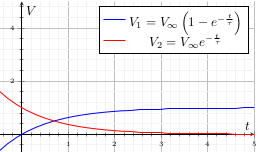
\includegraphics[scale=0.8]{../Figuras/solPulso1.png}
 \caption{Soluciones para el pulso.}
 \label{fig:graficaX}
\end{figure}


Donde si estamos aplicando una corriente externa lo que sucede es lo que estamos viendo en azul, un exponencial que va creciendo y que tiende hacia un cierto valor límite que sería de infinito. Si dejamos de aplicar la corriente externa entonces ahora tendremos un exponencial, pero que tiende hacia el cero y se va a estabilizar en cero, lo que vemos en rojo. 

\begin{figure}[h]
 \centering
 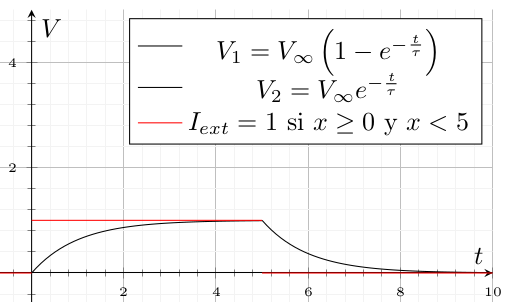
\includegraphics[scale=0.5]{../Figuras/solPulso2.png}
 \caption{Soluciones para el pulso escalón.}
 \label{fig:graficaX1}
\end{figure}

Simulando lo que hicieron Hodgkin y Huxley que fue al axón de repente darle un toque, siendo en el origen de la gráfica (que visualizamos en la figura \ref{fig:graficaX1}) la parte en la que le están dando el toque al axón, momentos antes estaba quieta la neurona de repente le aplican una cierta cantidad de electricidad y va a empezar a cambiar el comportamiento de los canales la porosidad de la membrana, vamos a ver que empieza a incrementarse la diferencia de potencial hasta que llegan a un nuevo equilibrio (alrededor de t = 3) y si siguieran dándole el toque en esa cantidad se quedaría ahí la neurona, ya no veríamos más cambios lo que va a suceder entonces es que, retiramos las pinzas (se le deja de dar el toque) y los canales otra vez van a empezar a regresar a la normalidad y vamos a ver un descenso en adelante.

Entonces hasta aquí ya tenemos la idea de cómo va a reaccionar la neurona ante cierto estímulo; sin embargo, esto que acabamos de ver en las gráficas sería como si tuviéramos un solo tipo de canal, ahora qué pasa si consideramos que tenemos diferentes tipos de canales pasando iones, en condiciones distintas. 
Aquí es donde va a importarnos el hecho de que existen diferentes tipos de canales con voltajes de equilibrio diferente. 
Retomando a los potenciales de Nerst \(E_{Na},E_{K},E_{L}\) notemos que están dados por:


\begin{equation}
    E = \dfrac{k_{B}T}{zq}\ln\dfrac{[adentro]}{[afuera]}
 \label{eq:diferenciaP}
\end{equation}

Estos potenciales están relacionados con las características termodinámicas, en la ecuación anterior \ref{eq:diferenciaP} \(k_{B}\) la constante de Boltzman, \(q\) es la carga del ion, y \(z\) es el número de iones. El logaritmo natural representando el promedio de cuántos elementos tenemos en la parte de adentro con respecto a cuántos elementos tenemos en la parte de afuera.

Considerando los diferentes puntos de equilibrio en los cuales se puede encontrar la diferencia de potencial en la membrana, vamos a distinguir entre tres estados de esta (también se puede ver en \ref{fig:graficaP}):

\begin{enumerate}
 \item \textbf{Polarizada} en su estado de reposo con \(V < 0 ( V \approx -70 mV )\).
 \begin{itemize}
  \item Su estado de reposo,cuando la neurona no está haciendo nada simplemente están corriendo los sodios y entran los potasios.
 \end{itemize}
 \item \textbf{Despolarizada} cuando \(V \geq 0\).
 \begin{itemize}
  \item Cuando en sus dendritas y en el cuerpo de la neurona se acumula una carga muy grande (un voltaje eléctrico, disparo), se abre la compuerta de sodio y van a empezar a entrar el sodio, esta diferencia de potencial que existía entre lo fuera y lo adentro se va a reducir de hecho se puede llegar a reducir bastante dependiendo de la carga que se le aplique.
  \item Iones positivos entran a la membrana.
  \item Valores positivos en la diferencia de potencial.    
 \end{itemize}
 \item \textbf{Hiperpolarizada} cuando la diferencia de potencial incrementa su magnitud \(V << 0\).
 \begin{itemize}
 \item En cuanto se despolarice van a empezar interacciones entre los diferentes tipos de canales que lo que van a intentar hacer es regresar a la neurona en su estado normal.
 \item Los canales de potasio abren sus compuertas, provocando que salga el potasio que está dentro del axón (en el citoplasma). 
 \item Iones positivos salen de la membrana.
 \item Si antes estaba quieta a los - 70mV, ahora va a quedar todavía más abajo alrededor de - 90mV. Esto va a permitir un fenómeno que se le conoce como \emph{el periodo de refracción} y ese periodo sirve para que simplemente se lance un disparo y que el comportamiento eléctrico no se rebote otra vez en dirección contraria en la neurona, va a quedar muy quieta la neurona durante un rato y después regresará otra vez a su estado de equilibrio. 
 \end{itemize}

\end{enumerate}
 
---

\section{Modelo de las compuertas iónicas controladas por voltaje}

Retomando el modelo del circuito eléctrico modelando la membrana, junto con los canales y los iones, volvamos a verlo ahora en la \ref{fig:circuito1}

\begin{figure}[H]
 \centering
 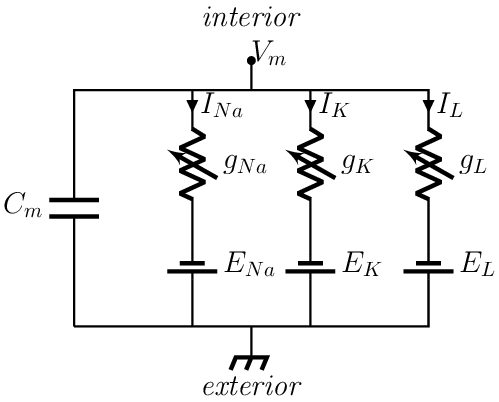
\includegraphics[scale=0.5]{../Figuras/circuito.png}
 \caption{Modelo de la membrana axónica modelada como circuito eléctrico, con los distintos canales presentes y su voltaje de reposo.}
 \label{fig:circuito1}
\end{figure}

Recordemos brevemente las definiciones de los dos tipos de canales protagonistas en el modelo:

\begin{definition}
 \emph{Canal persistente} Tiene un solo tipo de compuerta y dos estados posibles:
 \begin{enumerate}
  \item \textbf{Activado}
  \item \textbf{Desactivado}
 \end{enumerate}

\end{definition}

\begin{definition}
 \emph{Canal transitorio} Tiene compuertas de activación e inactivación, y tres estados:
 \begin{enumerate}
  \item \textbf{Activado} Ambas compuertas abiertas.
  \item \textbf{Desactivado} Compuerta de activación cerrada, inactivación abierta.
  \item \textbf{Inactivado} Compuerta de inactivación cerrada.
 \end{enumerate}

\end{definition}


Y retomando \hyperlink{LaEq}{la primera ecuación diferencial} donde tenemos, por un lado, la corriente que está pasando a través del capacitor, por otro lado, vamos a tener las corrientes que están circulando a través de los diferentes canales, 

\begin{equation}
  C_{m} \dfrac{dV_{m}}{dt} = - g_{Na} m^3 h(V_{m} - E_{Na}) - g_{K} n 4 (V_{m} - E_{K}) - g_{L} (V_{m} - E_{L}) + I_{ext}
  \tag{\ref{eq:corrientesEnLaMembrana2}}
\end{equation}

Las capacitancias y variables del lado izquierdo están explicadas en la sección \hyperlink{secc}{\emph{Modelo de la membrana como bicapa de lípidos}}, aquí vamos a retomar las ecuaciones \ref{eq:corrientesEnLaMembrana3},\ref{eq:corrientesEnLaMembrana4},\ref{eq:corrientesEnLaMembrana5} de esa misma sección, (recordemos que estás ecuaciones describen la probabilidad de que los canales iónicos estén abiertos) que son las siguientes:

\begin{equation}
  \dfrac{1}{\gamma(T)}\dfrac{dn}{dt} =  \alpha_{n^\infty} (V)(1 - n) - \beta_{n} (V) n = \dfrac{n(V)-n(t)}{\tau_{n}(V)}
  %\label{eq:probabilidades1}
  \tag{\ref{corrientesEnLaMembrana3}}
\end{equation}

\begin{equation}
  \dfrac{1}{\gamma(T)}\dfrac{dm}{dt} =  \alpha_{m} (V)(1 - m) - \beta_{m} (V) m = \dfrac{m^\infty(V)-m(t)}{\tau_{m}(V)}
  %\label{eq:probabilidades2}
  \tag{\ref{corrientesEnLaMembrana4}}
\end{equation}

\begin{equation}
  \dfrac{1}{\gamma(T)}\dfrac{dh}{dt} =  \alpha_{h} (V)(1 - h) - \beta_{h} (V) h = \dfrac{h^\infty(V)-h(t)}{\tau_{h}(V)}
  \tag{\ref{corrientesEnLaMembran53}}
\end{equation}

Ahora notemos los elementos en estas ecuaciones anteriores con \(ion\) pudiendo denotar las compuertas del potasio \(n\) o del sodio, ya sea \(m\) o \(h\):
\begin{itemize}
 \item \(\dfrac{1}{\gamma(T)}\) Este es el coeficiente de escala temporal, dependiente de la temperatura los por eso está apareciendo aquí una \(t\). Para las simulaciones que nosotros vamos a hacer vamos a pensar que estamos en una temperatura fija. 
 \item \(\alpha_{ion}(V)\) probabilidad de que una compuerta transite de cerrada a abierta.
 \item \(\beta_{ion}(V)\) probabilidad de que una compuerta transite de abierta a cerrada.
 \item \(ion^\infty(V)\) probabilidad de compuerta abierta en el equilibrio cuando \(t \rightarrow \infty\).
 \item \((ion)\) Probabilidad de que cada compuerta (n, m, h) esté abierta.
 \item \((1-ion)\) Probabilidad de que cada compuerta (n, m, h) esté cerrada.
 
 \item \(\tau_{ion}(V)\) Tiempo que toma llegar al equilibrio.
\end{itemize}


Lo que vamos a ver es que forma de escribir la ecuación depende precisamente del número de compuertas que tenían para poder abrirse y cerrarse. Reescribir la ecuación de esta manera lo que nos permite es medirlo en términos de estas probabilidades de que se abran y cierren las compuertas que serían 

Esta probabilidad se empieza a alterar conforme cambiamos el voltaje, pero no va a llegar a su valor de equilibrio sino hasta después de pasado un cierto periodo.


\section{Dinámica del voltaje durante un disparo} 

Ahora qué pasa cuando tomamos en cuenta que todas las compuertas están reaccionando al mismo tiempo.
Notemos primeramente como está reaccionando la membrana ante un impulso eléctrico o voltaje, en la siguiente imagen \ref{fig:voltaje1}.

\begin{figure}[h]
 \centering
 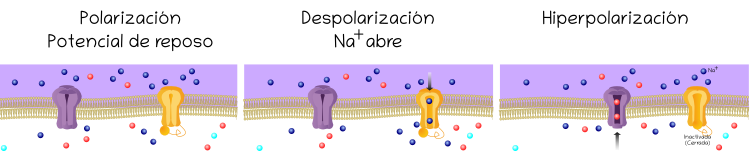
\includegraphics[scale=0.5]{../Figuras/polarizacion1.png}
 \caption{En la primera parte los canales están en un estado de reposo y la membrana está polarizada. En la segunda parte los canales han sido afectados por un impulso recibido desde el cono axónico, las compuertas de sodio se abren permitiendo el paso de iones de sodio al interior de la membrana y dejando a la membrana despolarizada. Momentos después la membrana llega a un estado de hiperpolarización donde intentará regresar al estado de equilibrio que tenía previamente, para esto la subpuerta de inactivación de sodio cerrará hasta no permitir el paso de sodio y el canal de potasio abrirá sus compuertas para dar salida a los potasios (iones positivos) que fluyan hacia el exterior de la membrana, así dejando el voltaje de la membrana incluso más negativo de lo que tenía durante su estado polarizado. }
 \label{fig:voltaje1}
\end{figure}

Ahora lo que vemos en la imagen \ref{fig:voltaje1} se gráfica de manera un poco más apegada a lo que pasa en los experimentos de la siguiente forma en la imagen \ref{fig:voltaje2}.

\begin{figure}[h]
 \centering
 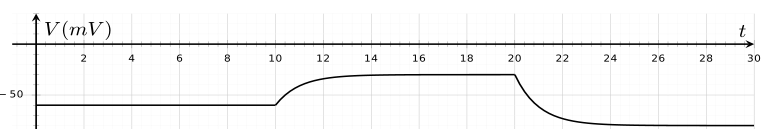
\includegraphics[scale=0.5]{../Figuras/polarizacion2.png}
 \caption{Gráfica del cambio de voltaje en la membrana dado un impulso atreves del tiempo. Cuando se rebasa el voltaje umbral, los canales de Na + y K + interactúan para producir una rápida despolarización de la membrana provocando una elevación del voltaje, para luego hiperpolarizarla. Durante el momento de despolarización la membrana puede llegar a valores positivos en este caso en particular el estímulo no es tan grande y se queda en valores negativos.}
 \label{fig:voltaje2}
\end{figure}


Ahora lo anterior está en términos de lo deseado, veamos entonces que paso en las mediciones de Hodgkin y Huxley con el axón en las siguientes gráficas \ref{fig:voltajeAB}, donde nos está mostrando como las subpuertas n y los factores \(\tau\), \(\alpha\) y \(\beta\) del canal de potasio se comportaron antes, durante y después del estímulo del voltaje. Recodemos que \emph{n} nos indica la probabilidad que las compuertas de potasio estén abiertas, este es un factor adimensional. \(\tau\) es el tiempo que tarda en llegar a un estado de equilibrio. \(\alpha\) y \(\beta\) las probabilidades que las compuertas del canal de potasio pasen de cerrados a abiertos y viceversa. 


Entonces notamos que en el mismo periodo de tiempo, la membrana está en reposo y conforme va recibiendo el voltaje incrementa la probabilidad que las compuestas de potasio estén abiertas, es decir \(n\) va incrementando conforme al estímulo, mientras que el estado de reposo es claramente alterado provocando que el valor \(\tau\) disminuya considerablemente. La probabilidad que las compuertas de potasio pasen de un estado cerrado a uno abierto durante el proceso (\(\alpha\)) aumenta prácticamente de forma exponencial, mientras que la probabilidad de que pasen de abierto a cerrado disminuye poco a poco. Con esto cumpliendo lo esperado en la dinámica del voltaje, al notar como está reaccionando el canal de potasio durante la polarización y despolarización (pulso). 



\begin{figure}[h]
 \centering
 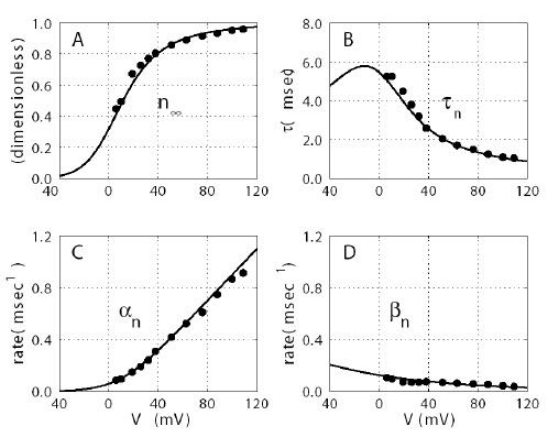
\includegraphics[scale=0.5]{../Figuras/medidasExperimentales.png}
 \caption{Medición experimental de los parámetros y ajuste manual de curvas. Imagen de Nelson 2004}
 \label{fig:voltajeAB}
\end{figure}

Con estas medidas experimentales ellos dan con curvas paramétricas ajustadas a los factores \(\alpha\) y \(\beta\) expresadas de la siguiente forma:

\begin{align*}
\alpha_{n}&=\dfrac{0.01(10-V)}{e^{\left(\dfrac{10-V}{10}\right)}-1}           &  \beta_{n}&=0.125e^{-\dfrac{V}{80}}\\
\alpha_{m}&=\dfrac{0.01(25-V)}{e^{\left(\dfrac{25-V}{10}\right)}-1}                    &  \beta_{m}&=4e^{-\dfrac{V}{18}}\\
\alpha_{h}&=0.07 e^{-\left(\dfrac{V}{20}\right)}              &  \beta_{h}&=\dfrac{1}{e^{\left(\dfrac{30-V}{10}\right)}+1}
\label{eq:curvas}
\end{align*}


Ahora veamos las gráficas de la dinámica del disparo pero ya con los las compuertas del potasio y sodio interactuando al mismo tiempo, en las figuras \ref{fig:voltajeActInac} y \ref{fig:voltajeActInac1}


\begin{figure}[h]
 \centering
 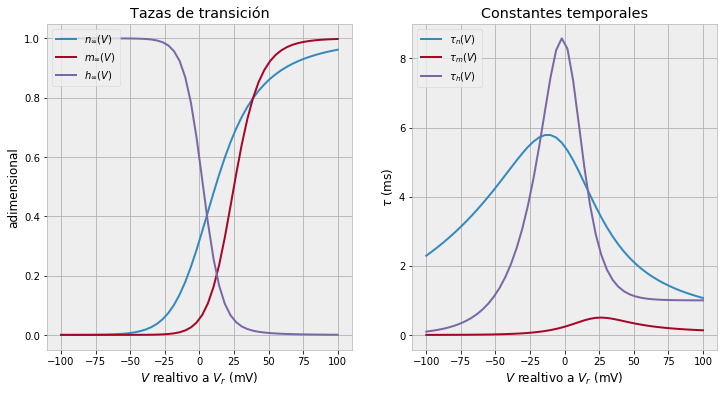
\includegraphics[scale=0.6]{../Figuras/actinac.png}
 %\caption{Activación e inactivación de los canales. Del lado izquierdo vemos que alrededor de los menos 50 mV aumenta la probabilidad que las compuertas de potasio abran y los potasios salgan, el sodio tarda un poco más en reaccionar para dejar entrar a los sodios, y la probabilidad que quede no bloqueado disminuye, hasta bloquear por completo a los iones de sodio alrededor de los 50 mV. Del lado derecho vemos como \(\tau\), va interactuando conforme al voltaje, el Na+ reacciona rápidamente ante él impuso pues regresa rápidamente a su estado de equilibrio, esto indica porque aún que el sodio abre sus compuertas, la compuerta de bloqueo se cierra rápidamente, dejando inactivado el canal, luego el K+ reacciona más lentamente para regresar a su estado de equilibrio dejando más tiempo activado el canal y salgan los potasios.}
 \label{fig:voltajeActInac}
\end{figure}


\begin{figure}[H]
 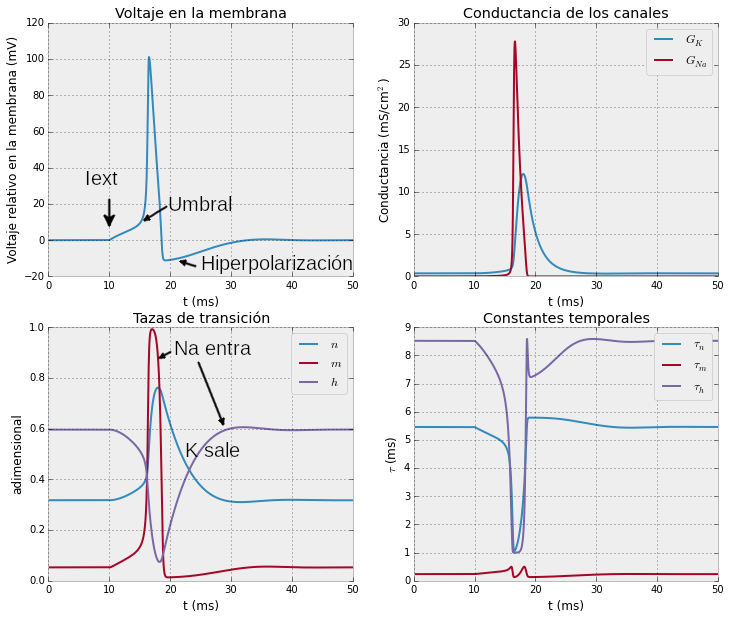
\includegraphics[scale=0.6]{../Figuras/disparo.png}
 \caption{Medidas experimentales del estímulo y la reacción de todos los componentes de la membrana. El origen en estás gráficas realmente esta representando el punto de equilibrio que es alrededor de los -70mV. Del lado superior izquierdo mostrando como cambia el voltaje de la membrana respecto al tiempo, del lado superior derecho el comportamiento de la conductancia de los canales mostrando que aunque la conductancia del sodio reacciona más, es más breve, mientras que el potasio reacciona en menor medida pero durante más tiempo. En la parte inferior derecha la taza de transición de las compuertas n,m y h, mostrando que en cuando llega el impulso el primero en reaccionar es el sodio permitiendo que entre muy brevemente el sodio e inactivandose casi inmediatamente después, mientras que en ese momento los potasios se están liberando hacia la parte exterior de la neurona. Finalmente del lado inferior izquierdo mostrando como se comporta las constantes temporales, mostrando que las compuertas de activación de sodio no son tan afectadas comparado a la compuerta de bloqueo, notando algunos cambio bruscos en esta, mientras que el potasio si se nota más afectado y durante más tiempo pero recuperándose sin cambios bruscos. }
 \label{fig:voltajeActInac1}
\end{figure}




\section{Simulación usando el método de Euler}

En esta sección se listará como estamos resolviendo las ecuaciones diferenciales, para tener una simulación numérica y se trata del algoritmo de integración \footnote{Hodgkin-Huxley Simulation Using Euler's Method lo puedes encontrar en la siguiente liga \url{https://webpages.uidaho.edu/rwells/techdocs/Biological\%20Signal\%20Processing/Chapter\%2003\%20The\%20Hodgkin-Huxley\%20Model.pdf}}. Las gráficas de la sección anterior se obtuvieron con el método de Euler que se describe más adelante.

\begin{algorithm}
  \caption{Algoritmo de integración de Euler [Wells pp51].}\label{AIE}
  \begin{algorithmic}[1]
    \Function{INTEGRADISPARO}{$T,\Delta T,V_{0},I_{ext}(t)$}
    \State Inicializar arreglos de longitud T: $T[],V[],n[],m[],h[],G_{Na}[],G_{K}[],\tau_{n}[],\tau_{m}[],\tau_{h}[] \gets arreglo[numeroDePasos] $
    \State  $V[0] \gets V_{0}$
    \For {$ t = 0  a  t = T cada \Delta t $}
        \State Calcular $\alpha_{n}, \beta_{n}, \alpha_{m}, \beta_{m},\alpha_{h}, \beta_{h} $ utilizando $V(t)$.
        \State Calcular las tres $\tau_{x} $ y $x^\infty $ apartir de las anteriores.
        \State Calcular las probabilidades de las compuertas $n, m, h, $ utilizando las ecuaciones en diferencias en su forma matricial $\Pi(t + \Delta t) = A_{\pi}\Pi(t) + B_{\pi}$.
        \State Calcular $G_{Na} = g_{Na}m^3h $ y $G_{K} = g_{K}n^4 $.
        \State Almacenar los resultados de este paso en los arreglos $T[], V[], n[], m[], h[], G_{Na}[], G_{K}[], \tau_{n}[], \tau_{m}[], \tau_{h}[] $
        \State $I_{ext} \gets I_{ext}(t) $
        \State Calcular $V_{m} (t + \Delta t) $
    \EndFor
    \State Devolver los arreglos $T[],V[],n[],m[],h[],G_{Na}[],G_{K}[],\tau_{n}[],\tau_{m}[],\tau_{h}[] $ con los resultados para los tiempos $[0,T] $
    \EndFunction
  \end{algorithmic}
\end{algorithm}


Comenzamos con un valor inicial y a partir de ahí empleamos las ecuaciones, para calcular las tangentes, aproximamos a la curva con su tangente.

Para la función \textproc{INTEGRADISPARO} necesitamos cuatro valores de entrada que van a provocar diferentes comportamientos:

\begin{enumerate}
 \item $T$ nos indica durante cuánto tiempo queremos correr la simulación.
 \item $\Delta T $ nos indica que tan finos queremos que sean los pasos recordemos que vamos a aproximar la función con segmentos de recta siguiendo la tangente. Si hacemos pasos demasiado pequeños nos vamos a tardar demasiado en hacer el cómputo.
 \item $V_{0} $ es el voltaje inicial en donde empieza nuestra simulación donde estaba en nuestra neurona cuando empezamos a trabajar.
 \item $I_{ext}(t) $ es la corriente externa, de qué magnitud fue el toque que le estamos dando en este momento al axón 

\end{enumerate}

A partir de los elementos iniciales proporcionados ya podemos calcular lo demás. Vamos a querer guardar lo que está ocurriendo para todos los tiempos desde cero hasta t en cada delta, y lo vamos a hacer en forma de arreglos donde en la posición [0], está la primera medición en t=0 y la posición t está la medición en el tiempo t. Vamos a tener toda una serie de puntos donde estamos guardando estos pasos para inicializarlo. 

Sabemos que necesitamos es un primer valor a partir del cual vamos a calcular la tangente y vamos a ir aproximando lo demás, entonces para eso queríamos \emph{el voltaje inicial}, como nosotros sabemos donde estaba en reposo nuestra célula originalmente, vamos a poder guardar ese voltaje como el primer valor para nuestra simulación. Ahora todos los demás elementos como $\alpha$s y $\beta$s y etc. se pueden calcular si ya conocíamos ese voltaje inicial, entonces a partir de este momento podemos repetir el mismo ciclo tantas veces como sea necesario para cubrir, el intervalo. 
Desde el tiempo inicial hasta el tiempo t, brincando de delta T en delta T. 
Entonces dado un voltaje vamos a calcular las diferentes \(\alpha\)s que son las que se medían experimentalmente originalmente utilizando las ecuaciones  de las curvas paramétricas ajustadas \ref{eq:curvas} (paso 5).

Ya calculadas las alfas y betas ahora si se puede calcular las $\tau$ , $n^{\infty}$, $m^{\infty}$, $h^{\infty}$ (paso 6).
Teniendo estas entonces podemos calcular las probabilidades para las compuertas n, m, h usando las ecuaciones en diferencias en forma matricial, estas matrices se pueden expresar como \ref{fig:matriX}.

\begin{figure}[H]
 \centering
 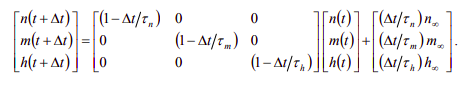
\includegraphics[scale=0.7]{../Figuras/matrix.png}
 \caption{Forma matricial para el cálculo de las probabilidades de las compuertas n, m, h.}
 \label{fig:matriX}
\end{figure}

Ahora esta parte fue importante sobre todo por el asunto de las pérdidas numéricas, recordemos que la computadora tiene una representación en punto flotante, lo cual quiere decir que un número real no se puede representar en la computadora, esto es importante por el problema del truncamiento, cada vez que se truncan dígitos al momento de calcular estamos perdiendo precisión, por esto es importante la forma en la que se procede a hacer los cálculos porque puede que se llegue a resultados un tanto distintos a los deseados aunque los cálculos sean correctos. 

Ya teniendo estos datos podemos fácilmente calcular las conductancias, simplemente sustituyendo los valores (paso 8).

Es bueno una vez que ya terminamos de calcular estos términos que se van a necesitar en la ecuación principal  \ref{eq:corrientesEnLaMembrana2} que es la del voltaje de la membrana,  ir almacenando en los \emph{resultados temporales} dentro de nuestros arreglos en la casilla que les corresponda, para ese momento (paso 8). En el paso 9, es donde ya vamos a utilizar \emph{la corriente externa} para meterla en la ecuación diferencial para el voltaje. Una vez que tengamos esto tenemos que repetirlo para cada paso, se está calculando el tiempo t,  entonces conforme avance el tiempo, va a dar el siguiente valor del voltaje, ya teniendo el siguiente valor del voltaje se va a poder usar para el siguiente paso ("como valor inicial nuevo") y así nos vamos a seguir todo el tiempo. 
Terminando el tiempo asignado a la simulación, tenemos ya los arreglos llenos de los datos que nos van a poder permitir graficar, qué fue lo que sucedió en cada tiempo, con cada canal y es precisamente  así que se puede graficar las mediciones presentadas en la sección anterior.


\chapter{Aprendizaje de máquina}
\section{Introducción}

En este capitulo se desarrolla el procesos que pasa una maquina para que \emph{aprenda}, para esto notemos el concepto de aprender. En lo seres humanos se denota como el hecho de adquirir el conocimento de algo mediante el estudio o la experiencia a partir de ejemplos específicos en nuestro medio, entonces aquellos problemas que inicialmente no pueden resolverse, puedan ser resueltos después de obtener más información acerca del problema. Desde pequeños empezamos por aprender por palabras (conceptos) que asociamos con algo especifico, para después relacionar que varios objetos pertenecen a un tipo de conjunto y otros no. Como que un muñeco, una pelota y unos bloques de construcción de plastico, pertecen a un conjunto denotado como "juguetes", y que plato, taza, y tazón no pertecen a este conjunto sino al conjunto "vajilla". Entonces para organizar los conceptos que vamos aprediendo hacemos uso de una función booleana, donde la entrada es el concepto, la pregunta es, ¿Este objeto pertence a un cierto conjunto de objetos con características similares? y la salida es falso o verdadero. A este proceso, se le conoce como \emph{aprendizaje de conceptos} y en este curso lo simplificamos como \emph{función boleana de aproximación mediante ejemplos}.

Ahora lo que denotamos como el hecho que una maquina aprenda, lo vemos como cualquier programa que mejore su desempeño en alguna tarea mediante la experiencia. Con más formalidad se denota como:

\begin{definition}
 \textbf{Apredizaje maquina:} Se dice que un programa de computadora aprende, si su desempeño en T, medido por P , mejora con la experiencia E. Tal que: 

 \begin{itemize}
  \item \emph{T} es un tipo de tarea.
  \item \emph{P} es una medida de desempeño.
  \item \emph{E} la experiencia con ejemplos (entrenamiento).  
 \end{itemize}

 , \footnote{Machine Learning, Mitchell 1997, pag. 14.}.
\end{definition}

Algunos ejemplos para definición anterior pueden ser los siguientes:
\begin{itemize}
  \item \emph{T}, como:
   \begin{itemize}
    \item Jugar un juego de mesa.
    \item Clasificar varios tipo de hojas.
    \item Reconocer una voz en particular.
   \end{itemize}
  \item \emph{P}, como:
    \begin{itemize}
     \item Porcentaje de juegos ganados en las partidas.
     \item Porcentaje de hojas correctamente clasificadas.
     \item Porcentaje de reconocimiento de timbre de la voz.
    \end{itemize}
  \item \emph{E}, como:
    \begin{itemize}
        \item Jugar juegos de práctica.
        \item Una secuencia de imagenes etiquetadas.
        \item Una secuencia de audios etiquetados.
    \end{itemize}

\end{itemize}


A partir de ahora nos dedicaremos a definir correctamente tareas que nos interese que un programa aprenda, para entender la forma más abstracta del problema y así proponer los algoritmos que nos ayuden a resolverlo.

Consideremos también que los sistemas de redes neuronales artificiales son un tipo de algoritmo para la representación del proceso de aprendizaje. Un problema de aprendizaje bien definido requiere una tarea bien especificada, medidas de desempeño y datos para obtener experiencia. 

El aprendizaje maquina se apoya de disciplinas, como la inteligencia artificial, probabilidad, estadística, complejidad computacional, psicología, neurobiología y filosofía.

Para proponer un algoritmos de aprendizaje automático necesitamos, elegir el tipo de experiencia de entrenamiento, definir la función objetivo a aprender y un algoritmo para aprender la función objeto a partir de ejemplos de entrenamiento.

Los algoritmos de aprendizaje maquina han sido utilizados apliamente por la industria bancaria, por gobiernos y por su puesto por el area de la salud. En la industria bancaria por ejemplo, donde es necesario aprender las reglas generales para determinar la solvencia crediticia, a partir de las bases de datos. Por los gobiernos para el reconocimiento de rostros humanos a partir de imágenes. En el area de salud para a partir de bases de datos de pacientes descubrir automaticamente regularidades implicitas en los resultados de tratamientos.






\section{Espacio de Hipotesis}

El aprendizaje automático, es utilizar datos disponibles para, aprender una tarea mediante una función que mejor mapee entradas a ciertas salidas. A esto se le llama  aproximación de función, en el que aproximamos una función de destino desconocida (que suponemos que existe) que puede asignar mejor las entradas a las salidas en todas las observaciones posibles del dominio del problema.

Una función de un modelo que se aproxima a la función objetivo y realiza asignaciones de entradas a salidas se denomina hipótesis.

Ahora estas funciones pueden tener formas muy generales en el aprendizaje de máquina pueden tener forma, por ejemplo, de estructuras de datos, como los árboles de decisión, donde cada nodo pregunta si o no, pertenece una clasificación.
pueden ser también funciones matemáticas como el caso de las redes neuronales, entonces la forma que tomen estas hipótesis en general puede abarcar muchos métodos y estructuras. 

Entonces el aprendizaje consiste en, explorar un espacio de posibles hipostesis para encontrar la hipotesis (una función) que mejor encaje, deacuerdo a lo se obtuvo en los ejemplos de entrenamiento, y predecir alguna característica de salida deseada. Usualmente se denotan como sigue:

\begin{itemize}
 \item \emph{h} (hipótesis): una sola hipótesis, por ejemplo una instancia o modelo candidato específico que asigna entradas a salidas, se puede evaluar y se usa para hacer predicciones.

 \item \emph{H} ( conjunto de hipótesis ): Un espacio de posibles hipótesis para mapear entradas.
 \end{itemize}


Una breve ejemplo para denotar un espacio de hipostesis sería el problema es saber los días que nos conviene ir al cine,
donde nuestra tarea T es aprender a predecir el conjunto de dias que nos conviene ir al cine, basado en los atributos de los dias, donde cada hipotesis la representaremos apartir de un conjunto de atributos de las instancias (dias), estonces cada hipotesis es un vector con tres atributos, \emph{tiene2x1, esEstrenoDePelicula, actoresConocidos}. Para cada atributo de la hipotesis tendría uno de los siguientes valores; $Si, No, ?$. Donde ? indica que cualquier valor es valido para ese atributo.

Cuando alguna instancia $x$ cumpla con todos los atributos de una \(h\), entonces \(h(x) = 1 \) y $x$ es un ejemplo positivo. Entonces para representar la hipostesis, que nos conviene ir solo los dias con 2x1, y que hay peliculas donde los actores son conocidos, la escribimos como $h(\textlangle Si, ?, Si\textrangle) = 1 $, la hipotesis que cualquier día nos conviene ir al cine la denotamos como $h(\textlangle ?, ?, ?\textrangle) = 1 $, nuestra función objetivo la denotamos como una función booleana $c:X \rightarrow {0,1} | X, el conjunto de los 365 dias del año$, entonces $c(x) = 1$ cuando en los datos nos dicen que con la instancia x conviene ir al cine, $c(x) = 0$ en caso que no. Por tanto para aprender la tarea T, necesitamos \emph{una hipotesis h en H tal que h(x) = c(x) para todas las x en X }. La tarea de aprendizaje del concepto $c$ requiere aprender el conjunto de instancias que lo satisface, describiendo este conjunto mediante una conjunción de restricciones sobre los atributos de la instancia.  

Estas hipotesis (funciones) pueden llegar a ser sumamente complejas y tener que mapear datos de entrada con muchas formas ej. imagenes, trayectorias, etc. En el caso de las redes neuronales, el espacio de hipótesis está determinado por la arquitectura de la red.
Vamos a definir el espacio de hipótesis, cuando decidamos qué neuronas vamos a poner en nuestro sistema, como las conectamos entre sí y cómo van a transferirse información de una a la otra y cuántas neuronas van a ser. Lo que veremos a lo largo del curso son diferentes arquitecturas y el impacto que tiene hacer diferentes modificaciones así como las matemáticas que existen detrás de estas. 


\section{Clasificación de los conjuntos de datos}

La experiencia \(E\) para aprender la vamos a obtener mediante un conjunto datos, llamados datos de entrenamiento, estos se separan en tres bloques:

\begin{itemize}
 \item \textbf{Entrenamiento:} Datos con los cuales se ajustan los parámetros de la hipótesis (del \(50\%\) al \(80\%\) de los datos). En este bloque se escoje que función del espacio fue mejor para el aprendizaje.
 
 \item \textbf{Validación:} Datos utilizados para ajustar los parámetros (hiperpametros) del algoritmo de entrenamiento, que puedan afectar qué hipótesis es seleccionada (del \(25\%\) al \(10\%\) de los datos y no deben ser usado durante el entrenamiento). Un ejemplo de un hiperparámetro para redes neuronales son el número de nodos ocultos en cada capa.

 \item \textbf{Prueba:} Datos utilizados para evaluar la posibilidad de que la hipótesis aprendida generalice \footnote{Se desea que nuestro modelo de aprendizaje, una vez entrenado con datos que ya hemos visto, se pueda usar con datos nuevos. Para ello debemos asegurarnos que el modelo no ha simplemente memorizado las muestras de entrenamiento, sino que ha aprendido propiedades del conjunto.} a datos no vistos anteriormente. Esta porción que se mantiene aparte. Con estos se evalua el modelo, se reporta la eficacia del modelo según los resultados en este conjunto (del \(25\%\) al \(10\%\) de los datos).

\end{itemize}

\emph{El conjunto de datos de entrenamiento se usa para aprender una hipótesis y el conjunto de datos de prueba para evaluarla.}

\subsection{Tipos de aprendizaje}

\begin{description}
 \item [Aprendizaje Supervisado], el modelo usa datos etiquetados a una respuesta especifica(labaled data), durante el entrenamiento se intenta encontrar una función que aprenda a asignar los datos de entrada (input data) con los datos en el etiquetado. Para depues predecir una relación, dado un dado totalmente nuevo para el modelo. Los modelos pueden ser:
    \begin{itemize}
    \item Regresión: Un modelo de regresión busca predecir valores de salida continuos. Por ejemplo, en predicciones meteorológicas, de expectativa de vida, de crecimiento de población.
    \item Clasificación: En un problema de clasificación se desea predecir una salida discreta. Por ejemplo, identificación de dígitos, diagnósticos.
    \end{itemize}

 \item [Aprendizaje no supervisado], es usado cuando no se tienen datos “etiquetados” para el entrenamiento. Solo sabemos los datos de entrada. Por tanto, únicamente podemos describir la estructura de los datos, para intentar encontrar algún tipo de organización que simplifique un análisis. Por ello, no se tienen valores correctos o incorrectos (es utilizado para aprender de una manera autoorganizada).
 
 \item [Aprendizaje por refuerzo], inspirado en la psicología conductista; donde el modelo aprende por sí solo el comportamiento a seguir basándonos en \emph{recompensas y penalizaciones}. Este tipo aprendizaje se basa en mejorar la respuesta del modelo usando un proceso de retroalimentación (\emph{feedback}). Su información de entrada es el feedback que obtiene del mundo exterior como respuesta a sus acciones. A aprende a base de ensayo-error.
 
\end{description}


Mientras que el aprendizaje supervisado y el no supervisado aprenden a partir de datos obtenidos en el pasado, el aprendizaje por refuerzo aprende desde cero, es decir, con un estado inicial y son su ambiente, va aprendiendo a futuro, mediante posibles penalizaciones o recompensas.  El \emph{aprendizaje por refuerzo} es usado en videojuegos porque cada vez que se realizan las acciones correctas se ganan puntos y entonces se entrena a la gente para que pueda conseguir la mayor cantidad de puntos. En este siempre hay: un agente, un ambiente definido por estados, acciones que el agente lleva a cabo (que le llevan de un estado a otro), y recompensas o penalizaciones que el agente obtiene.

En cada acción, el agente solo conoce el estado en el cual se encuentra y las acciones posibles que puede elegir a partir de ese estado. No sabe si llegando al siguiente estado, obtendrá mejores o peores recompensas, irá aprendiendo en cada estado qué acciones lo llevará a obtener una mayor recompensa a largo plazo, y que el valor de las acciones en ese estado puedan subir. \emph{Se enfoca en que el agente aprenda una política óptima para alcanzar el objetivo.} El agente siempre está en fases de \emph{exploración} y \emph{explotación}, en la fase de exploración el agente toma una acciones de manera aleatoria, y en la de explotación va a tomar acciones basándose en cuán valiosa es realizar una acción a partir de un estado dado.

En plataforma de ventas en línea es donde podemos encontrar este tipo de modelo que están entrenados con este tipo de aprendizaje, donde al iniciar la sesión no conoce nada del usuario, solamente tiene un ambiente dado por los productos de la plataforma y su estado inicial es cero, para hacer individual la experiencia del usuario y que compre más. El algoritmo realiza la acción de mostrar ciertos productos (algún estado) si el usuario da clic a estos productos, el agente recibirá un punto de recompensa, por lo cual pasará a otro estado donde ofrecerá productos del mismo estilo donde pueda maximizar una venta, así sé ira adaptando a cada usuario.

%\section{Conjuntos de entrenaiento, validación y prueba}


\part{Redes dirigidas acíclicas}
\chapter{Perceptrón simple}
\section{Perceptrón}

El perceptrón fue la primera red neuronal artificial (o ANS, Artificial Neural Systems) descrita algoritmicamente. En las decadas de los 60's y 70's, los popularizo el psicólogo Franck Rosenblatt, en su libro llamado Principios de neurodinámica, donde presentó varios modelos de perceptrones, en el Laboratorio Aeronáutico de Cornell en Estados Unidos, originalmente estaba diseñado para ser una máquina, en vez de un algoritmo. Estaba diseñado especificamete para el reconocimiento de imagenes donde, cada peso era un cable físico por pixel de entrada, este erá una matriz de 200 x 200, conectados aleatoriamente a las "neuronas", las actualizaciones de los pesos se realizarón mediante motores eléctricos. 

El perceptrón es en sí, es la representación de un sola neurona, este se ocupa para la clasificación de patrones en un conjunto de datos multivariados, con ese se obtienen fronteras lineales en el plano, mediante un algoritmo de aprendizaje que veremos más adelante.

Recordando, una neurona es un celula elemental que a partir de un vector de entrada procedente del exterior o de otras neuronas (estimulo), proporciona una única respuesta (si activo el potencial de acción o no), ver figura \ref{fig:unaNeurona}. Los elementos que actuan en una neurona los podemos listar como:
\begin{itemize}
 \item \textbf{Entradas:} $x_{j}(t)$. Las variables de entrada y salida pueden ser binarias (digitales) o continuas (analógicas) dependiendo del modelo de aplicación.
 \item \textbf{Pesos sinápticos:} $w_{ij}$. Representan la intensidad de interacción entre cada neurona presináptica j y la neurona postsináptica i.
 \item \textbf{Regla de propagación:} $h_{i}(t) = \sigma(w_{ij}, x_{j}(t))$. Proporciona el valor del potencial postsináptico, de la neurona i en función de sus pesos y entradas. 
    \begin{itemize}
     \item $h_{i}(t) = \sum_{i=0}^{n} w_{ij} x_{i} $, Es una suma ponderada de las entradas con los pesos sinápticos.
      Así, si la entrada es positiva, dependiendo de los pesos podemos saber si fue una sinapsis excitadora (pesos positivos) o inhibidora (pesos negativos).
    \end{itemize}

 \item \textbf{Función de activación o de transferencia:} $a_{i}(t)$ Proporciona el estado de activación actual, de la neurona $i$ en función de su estado anterior, $a_{i}(t-1)$ y de su potencial postsináptico actual. 
    \begin{itemize}
     \item $a_{i}(t) = f_{i}(a_{i}(t-1),h_{i}(t))$, es la que usalmente se usa.
     \item $a_{i}(t) = f_{i}(h_{i}(t))$, en algunos modelos solo se concidera que el estado actual no dependende del tiempo anterior.

     \end{itemize}

 \item \textbf{Función de salida: } $F_{i}(a_{i}(t))$ Da la salida actual, $y_{i}(t)$, de la neurona i en función de su estado de activación actual. El estado de activación de la neurona se considera como la propia salida. 
    \begin{itemize}
     \item $y_{i}(t) = F_{i}(a_{i}(t))$
     \item $y_{i}(t) = F_{i}(f_{i}(a_{i}(t-1),\sigma(w_{ij},x_{j}(t))))$
    \end{itemize}

\end{itemize}


\begin{figure}[h]
 \centering
 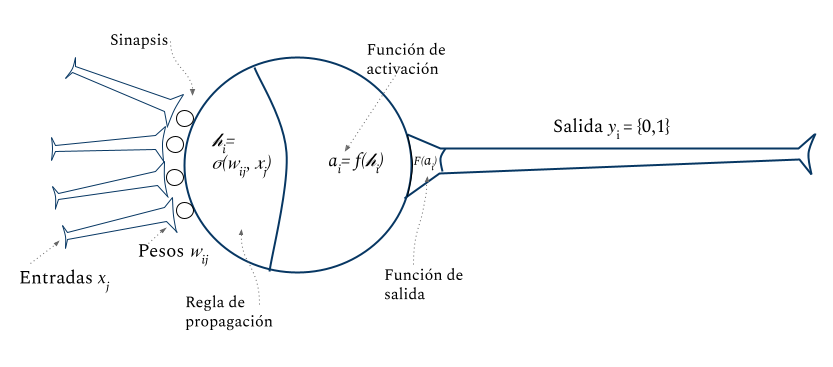
\includegraphics[scale=0.5]{../Figuras/Percp.png}
 \caption{Neurona vista como un modelo artificial (perceptrón).}
 \label{fig:unaNeurona}
\end{figure}


Un perceptrón toma un vector de entradas de numeros reales, calcula una combinación lineal de estas entradas, luego emite un 1 si el resultado es mayor que algún umbral y -1 de lo contrario. 
Es decir, dadas las entradas $x_{1}... x_{n}$, la salida $o(x_{1}. ..., x_{n})$ calculada por el perceptrón es 1 si $w_{0} + w_{1}x_{1} + w_{2}x_{2} + ... + w_{n}x_{2} > 0 $ y -1 de lo contrario, donde cada $w$ es una constante $\mathbb{R}$, un peso, que determina la contribución de la entrada $x$ a la salida del perceptrón.  La constante $w_{0}$ es un \emph{umbral} (bias) que la suma de las entradas con los pesos debe superar para que el perceptrón emita un 1. En otras palabras es un peso que va a actuar junto con una entrada de valor $1$, que vamos a poder ajustar para que nuestrá función de activación, se mueva de derecha a izquierda en el plano para ayudarnos a ajustar nuestros resultados, provocando un gran impacto en el aprendizaje. Esto se muestra en la siguientes graficas \ref{fig:bias}. Más adelante hablaremos de su regla de entrenamiento (Training rule).

\begin{figure}[h]
    %\centering
    \subfloat[Función sigmoide.]{
            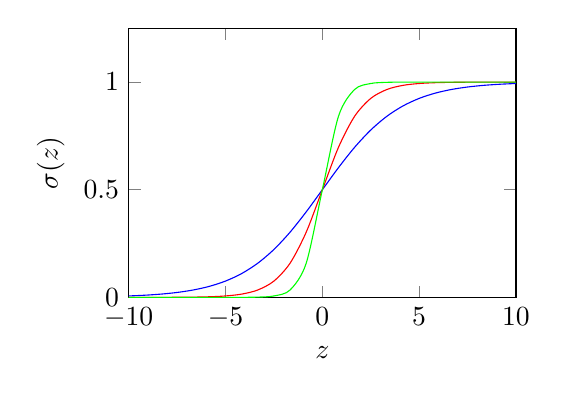
\begin{tikzpicture}
            \begin{axis}[width=6.5cm,height=5cm,ylabel=$\sigma(z)$,xlabel=$z$,ymin=0,ymax=1.25,xmin=-10,xmax=10]
                \addplot[domain=-10:10,blue,smooth] {1/(1+exp(-(x*.5)))};
                \addplot[domain=-10:10,red,smooth] {1/(1+exp(-(x* 1)))};
                \addplot[domain=-10:10,green,smooth] {1/(1+exp(-(x* 2)))};
                %\addlegendentry{$y = \dfrac{1}{1+e^{-x}}$}
            \end{axis}
        \end{tikzpicture}
    }
    \subfloat[Función sigmoide con bias.]{
            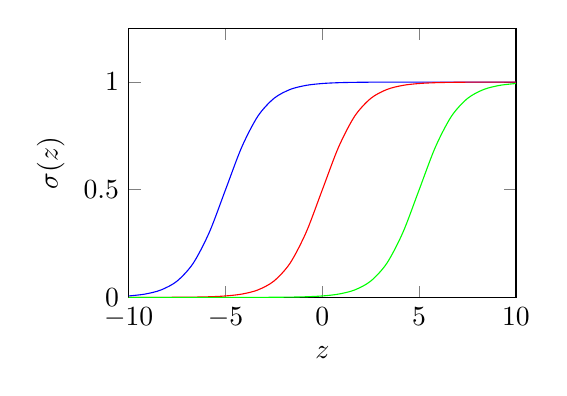
\begin{tikzpicture}
            \begin{axis}[width=6.5cm,height=5cm,ylabel=$\sigma(z)$,xlabel=$z$,ymin=0,ymax=1.25,xmin=-10,xmax=10]
                \addplot[domain=-10:10, blue,smooth] {1/(1+exp(-(x*1 + 5)))};
                \addplot[domain=-10:10, red,smooth] {1/(1+exp(-(x* 1)))};
                \addplot[domain=-10:10, green,smooth] {1/(1+exp(-(x* 1 - 5)))};

                %\addlegendentry{$w = -5$}
            \end{axis}
        \end{tikzpicture}
    \label{fig:bias}
    }
    \caption[Impacto del bias]{
     Comportamiento de la función de activación (sigmoide) de un perceptrón con una sola entrada, \emph{(b)} el perceptrón sin el uso de bias, \emph{(b)} con el uso del bias, donde apesar de estár representandos con la misma entrada , el uso del bias afecta en los resultados de salida. Así si quisieramos que este perceptrón nos diera $y = 0$ con una entrada $x= 2$ sin el uso, ni ajuste del bias sería imposible, pues en (a) apesar que la gráfica azul está la entrada está ajustada con el peso $w=0.5$, la roja con el $w=1$, y la verde con el $w=2$  solo lo gramos alargarla un poco, haciendo que entradas que antes eran correctas ahora caigan $0$ también. Entonces lo que necesitamos es más bien "mover" la gráfica, esto lo logramos con la gráfica \emph{(b)} donde la entrada (única) está sumada con un bias (umbral) $x_{0}= 1$, ajustado en azul con peso $w_{0}= 5$, en rojo con $w_{0}= 0$, en verde con $w_{0}= -5$ y el peso $w_{1}=1$. Donde con $w_{0}= -5$ logramos nuestro objetivo de tener una salida $y=0$ con $x=2$. El bias nos permite mover la función fuera del origen.
     \label{fig:sigmoideBias}
     }
\end{figure}


El hecho de que un perceptrón aprenda implica elegir valores para los pesos denotados también por $\theta$.  Ahora, el espacio $H$ de las hipótesis candidatas consideradas en el aprendizaje del perceptrón, es el conjunto de todos los posibles vectores de pesos.  \[H = {\vec{w} |  \vec{w} \in \mathbb{R}^{n+1}}\].

\begin{figure}[h]
 \centering
 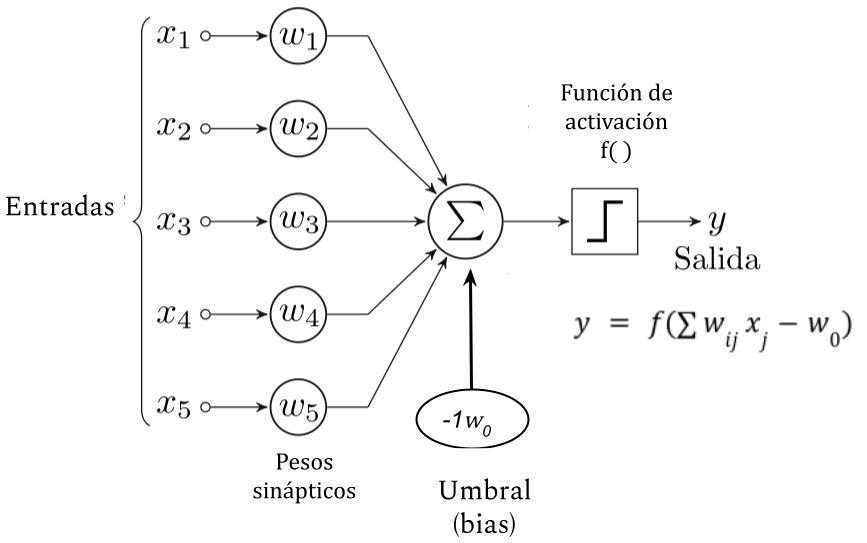
\includegraphics[scale=0.5]{../Figuras/Perceptron.png}
 \caption{Modelo estandar de un perceptrón.}
 \label{fig:unaNeurona2}
\end{figure}

Si bien en el momento que se publicó los logros con el modelo del percetrón las espectativas eran bastante altas, a medida de los años los cientificos Marvin Minsky and Seymour Papert desestiman en gran medida los alcances que realmente se puede tener con el perceptrón, al mostrar \footnote{ En 1969 publican Marvin Minsky y Seymour Papert que perceptrones de una sola capa (simples) solo son capaces de aprender a distinguir patrones linealmente separables, en el libro "Perceptrons".
} que no puede predecir operaciones lógicas que no sean linealmente separables, tal es el caso de la función XOR, que no es separable linealmente, siendo imposible que pueda aprender está función. Esto y el gran costo que representaba procesar todos los elementos que implicaba el entrenamiento, causa que por un buen tiempo se desetime el uso del perceptrón. Es hasta después de unas decadas que vuelve a tener relevancia con la propuesta de un perceptrón multicapa usando retropagación (Feedforward), siendo estos capaces de resolver la función XOR



\section{Compuertas lógicas con neuronas}
%operaciones lógicas

Aquí se muestra como se puede utilizar un perceptrón para simular compuertas lógicas tales como el or, not, and.

Para simular la compuerta \emph{not}, como está es una función boolean de \(B \rightarrow  B\), talque $not(x) = -x$ entonces en un plano de dos dimensiones, la podemos representar con dos puntos, el  $p_{1} = (0,0)$  y $p_{2} = (1,0)$donde $p_{1}$ representa cuando $not(0) = 1$, $p_{1}$ representa cuando $not(0) = 1$. Teniendo el espacio de la función definido lo que nos toca es, separar el plano para clasificar las entradas, este claramente se puede separar con un linea vertical, o con lineas con pendiente $1$ o $-1$. Para esta función solo necesitamos de una entrada y un sesgo (bias), donde la entrada la combinaremos con un peso, este peso lo asignaremos a tanteo (por la sencillez de la operación). Así el peso $w_{1} = -1$  y el peso asignado al bias sera $w_{0} = 0.5$, ahora con esto datos podemos:

\begin{itemize}
 \item Hacer la función de propagación donde $h(x) =  (x * -1) + (0.5) * 1 = 0.5 - x$
 \item Haccer la función de activación escalón $a(x) = sgn(h) = sgn(0.5-x)$ 
 \item Dar la salida donde $s(1) = sgn(0.5-1) = 0$ y $s(0) = sgn(0.5-0) =  1$, en este caso la salida es la identidad de la activación.
\end{itemize}

\begin{table}[H]
 \centering
\begin{tabular}{ | c | c |c | } 
 \hline
 $x$ &  $h$ & $s$ \\
 \hline
 $0$ &  $0.5$ & $1$ \\
 \hline
 $1$ &  $-1.5$ & $0$ \\
\hline
\end{tabular}
 
\end{table}


Algo similar va a pasar con la compuerta \emph{and} y \emph{or} donde al necesitar de dos entradas para la compuerta, asignaremos dos entradas para el perceptrón igualmente y las representaremos en el plano con cuatro puntos, donde cada punto representa una instancia y se le asigna valor positivo o negativo en el plano, así pues para el and tenemos los puntos $p_{1} = (0,0)$, $p_{2} = (0,1)$ , $p_{3} = (1,0)$, negativos y $p_{4} = (1,1)$ el único positivo. Así nos damos cuenta que necesitamos una recta con pendiente negativa y fuera del origen, que nos separe estás clases de puntos. Por tanto para el bias le asignamos un peso de $w_{0} = -1.5$, $w_{1} = 1$ y $w_{2} = 1$, con estos datos podemos: 


\begin{itemize}
 \item Hacer la función de propagación donde $h((x_{1},x_{2})) =  (x_{1} * 1) + (x_{2} *1) + (-1.5) * 1 = x_{1} + x_{2} - 1.5$
 \item Haccer la función de activación escalón $a((x_{1},x_{2})) = sgn(h) = sgn(x_{1} + x_{2} - 1.5)$ 
 \item Dar la salida donde $s = a(\vec{x})$, es la identidad de la activación.
\end{itemize}

\begin{table}[H]
 \centering
\begin{tabular}{ | c | c| c |c | } 
 \hline
 $x_{1}$ & $x_{2}$ & $h$ & $s$ \\
 \hline
 $0$ & $0$ & $-1.5$ & $0$ \\
 \hline
 $0$ & $1$ & $-0.5$ & $0$ \\
 \hline
 $1$ & $0$ & $-0.5$ & $0$ \\
 \hline
 $1$ & $1$ & $0.5$ & $1$ \\
\hline
\end{tabular}
 
\end{table}


Para la compuerta \emph{or} es algo muy similar pues podemos igualmente representar la función con cuatro puntos en el espacio cada uno representando una instancia, solo que ahora tres de estos puntos serán positivos y solo uno negativo, los puentos positivos serían $p_{2} = (0,1)$ , $p_{3} = (1,0)$ y $p_{4} = (1,1)$, mientras que $p_{1} = (0,0)$ negativo, el plano lo podemos dividir con una linea recta con pendiente negativa, así le asignamos $w_{0} = - 0.5$, $w_{1} = 1$ y $w_{2} = 1$, con esto hacemos los paso que ya sabemos:

\begin{itemize}
 \item Hacer la función de propagación donde $h((x_{1},x_{2})) = (x_{1} * 1) + (x_{2} *1) + (-0.5) * 1 = x_{1} + x_{2} + 0.5$
 \item Haccer la función de activación escalón $a((x_{1},x_{2})) = sgn(h) = sgn(x_{1} + x_{2} + -0.5)$ 
 \item Dar la salida donde $s = a(\vec{x})$, es la identidad de la activación.
\end{itemize}

\begin{table}[H]
 \centering
\begin{tabular}{ | c | c| c |c | } 
 \hline
 $x_{1}$ & $x_{2}$ & $h$ & $s$ \\
 \hline
 $0$ & $0$ & $-0.5$ & $0$ \\
 \hline
 $0$ & $1$ & $0.5$ & $1$ \\
 \hline
 $1$ & $0$ & $0.5$ & $1$ \\
 \hline
 $1$ & $1$ & $-1.5$ & $1$ \\
\hline
\end{tabular}
 
\end{table}


Tomando el hecho que en la naturaleza las neuronas van pasando información en una estructura que forma niveles de abstración, esto lo modelamos como capas de neuronas conectadas entre sí, cada capa haciendo su trabajo de abstración.
El perceptrón simple es un modelo neuronal unidireccional, una capa de entrada y otra de salida, que por si solo no puede separar todas la funciones lógicas pues tenermos el XOR, para resolver esto usaron perceptrones multicapa que se explicará más adelante en el curso.  

\section{Funciones de activación}

Recordando que la forma de las funciones de activación es $y = f(x)$, donde $x$ representa el potencial postsináptico e $y$ el estado de activación de la neurona, es decir si va a lanzar un disparo o no. Las funciones de activación más empleadas son:

\begin{figure}[h]
    \centering
    \subfloat[Función logistica.]{
            \begin{tikzpicture}
            \begin{axis}[width=5.5cm,height=4cm,ylabel=$\sigma(z)$,xlabel=$z$,ymin=0,ymax=1.25,xmin=-5,xmax=5]
                \addplot[blue,smooth] {1/(1+exp(-x))};
                \addlegendentry{$y = \dfrac{1}{1+e^{-x}}$}
            \end{axis}
        \end{tikzpicture}
    }
    \subfloat[Función tangente hiperbólica.]{
        \begin{tikzpicture}
            \begin{axis}[width=5.5cm,height=4cm,ylabel=$\tanh(z)$,xlabel=$z$,ymin=-1.25,ymax=1.25,xmin=-5,xmax=5]
                \addplot[blue,smooth] {tanh(x)};
                \addlegendentry{$y = \dfrac{e^{x}-e^{-x}}{e^{x}+e^{-x}}$}
            \end{axis}
        \end{tikzpicture}
    }\\
    \subfloat[Función escalón.]{
            \begin{tikzpicture}
            \begin{axis}[width=5.5cm,height=4cm,ylabel=$\sigma(z)$,xlabel=$z$,ymin=-0.1,ymax=1.25,xmin=-1,xmax=1]
                \addlegendimage{ultra thick,blue}
                \addplot[ultra thick,blue,mark=*,mark options={fill=white},samples at={-1.1,0}] {0};
                \addplot[ultra thick,blue,mark=*,samples at={0,1.1}] {0.5};
                \addlegendentry{$y=\begin{cases} 1 \quad &\text{si} \, x \geq 0 \\ 0 \quad &\text{si} \, x < 0 \\ \end{cases}$
            }   
            \end{axis}
        \end{tikzpicture}
    }
    \subfloat[Función lineal a tramos. Tangente hiperbólica rectificada.]{
        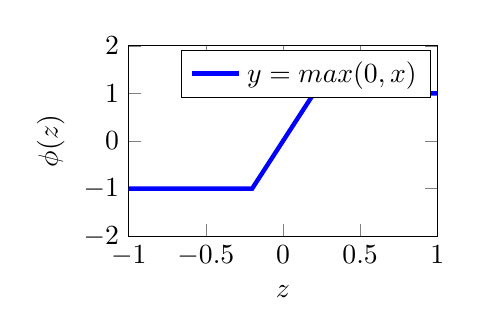
\begin{tikzpicture}
            \begin{axis}[width=5.5cm,height=4cm,ylabel=$\phi(z)$,xlabel=$z$,ymin=-2,ymax=2,xmin=-1,xmax=1]
                \addplot[blue,ultra thick] coordinates {(-1.1,-1) (-0.2,-1) (0.2,1) (1.1,1)};
                \addlegendentry{$y=max(0,x)$}
            \end{axis}
        \end{tikzpicture}
    }
        \caption[Funciones de activación sigmoides]{
        Las funciones de activación más usadas son la función sigmoide $\sigma(z)$ y la tangente hiperbólica $tanh(z)$.}
        \label{fig:sigmoid-tanh}
\end{figure}



\section{Funciones de error}

Entonces tomando como base el perceptrón, una vez obtenidas las salidas con una primera iteración nos daremos cuenta de que tan lejos o que tan cerca estuvimos de la respuesta correcta, con esto darnos la oportunidad de que pesos ajustar respecto a sus entradas, en la segunda iteración. Ahora para facilitarnos esto y tomando en cuenta que el entrenamiento consiste en varias iteraciones hasta llegar a aprender la tarea T, hacemos uso de una función de error que nos ayude a minimizar la diferencia de error en las salidas. 

Primero veamos el entrenamiento para una sola neurona, para esto haremos uso de la regla de aprendizaje del perceptrón (learning rule perceptron), donde para cada entrada, en la capa de salida se le calcula la desviación a la función objetivo. El cual utilizamos para ajustar los pesos del perceptrón (ver fig \ref{fig:errorP}). 

\begin{figure}[h]
 \centering
 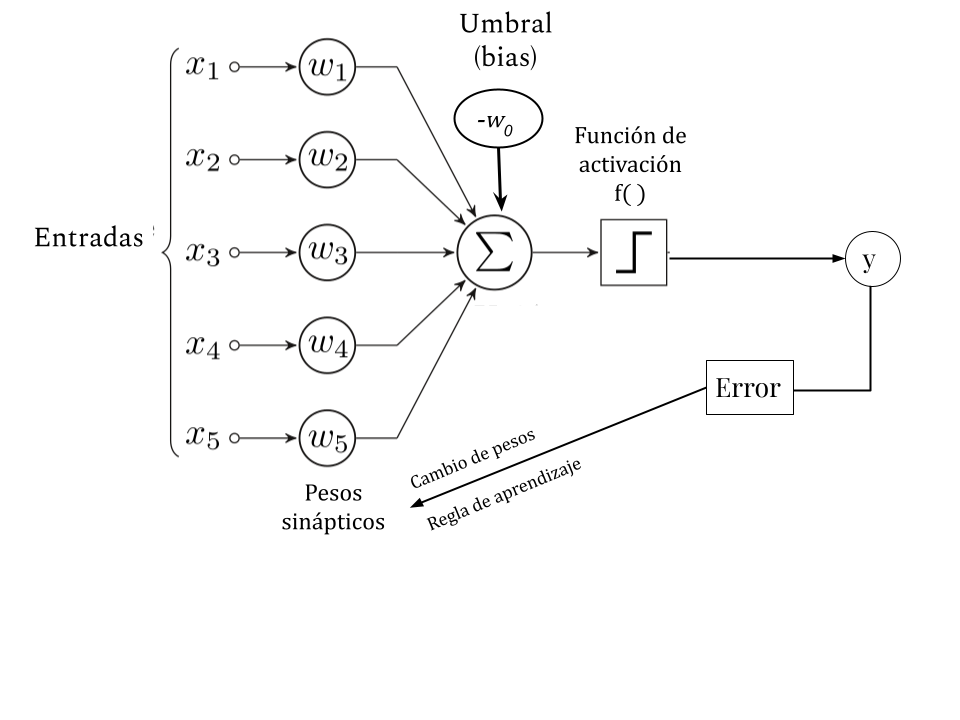
\includegraphics[scale=0.5]{../Figuras/ErrorPerceptron.png}
 \caption{Modelo estandar de un perceptrón.}
 \label{fig:errorP}
\end{figure}

Usualmente al principio del entrenamiento se asignan pesos aleatorios, a medida que avance el entrenamiento, se van modificando con cada iteración, así \(w_{i} \leftarrow w_{i} + \Delta w_{i}\). Esto con base a \emph{la regla de aprendizaje} donde: 

\begin{equation}
 \Delta w_{i} = \alpha(y - y_{out})x_{i}
\end{equation}

 
Con $y$ es la salida deseada, $y_{out}$ la salida generada, $\alpha$ la taza de aprendizaje (learning rate) y $x_{i}$ la entrada $i$. Lo que hace la taza de aprendizaje es moderar el grado en que los pesos son cambiados con cada iteración, se le asigna un valor muy pequeño (0.1 o 0.2) y conforme se logran ajustar los pesos se minimiza aún más. 


%Ahora supongamos que logramos que el perceptrón aprenda los datos
% de entrada, esto nos indica que $y = y_{out}$, haciendo que \
%(\Delta w_{i} = 0\), por tanto, ningún peso se actualice. En %nuestra etapa de validación, en un ejemplar nos de la salida $y = %-1$, cuando lo indicado es $1$. Entonces seguido de esa prueba %necesitamos hacer cambio de la taza de aprendizaje y renovación de %pesos aleatorios, para volver a ajustar los pesos correctamente y %no quede sobreajustada.


Para entrenar un perceptrón, utilizamos cualquier método de optimización de funciones para encontrar los parámetros $w$ que minimizan el error con alguna de las siguientes funciones de error:

\begin{description}
   
 \item \textbf{Diferencias al cuadrado}, también conocida como regla aprendizaje delta, es la suma de cuadrados de errores que se tuvieron con cada ejemplar el el conjunto de entranamiento. Los podemos decribir como: 
 
 \begin{equation}
   \dfrac{1}{2m}\sum_{m=0}^{M-1} (y_{m} - a_{m})^2
 \end{equation}
 
 con $y_{m}$ y $a{m}$, la salida obtenida dado un ejemplar $m$ y la salida correcta del ejemplar $m$ respectivamente.
 
 \item \textbf{Entropía cruzada.} Se usa para problemas de clasificación ya que su comportamiento es más suave (soft) y permite hacer clasificaciones más certeras. Se define como:

 \begin{equation}
  L (\Theta) = -\dfrac{1}{m}\sum_{M-1}^{m=0}(y^(m)log(a_{m}) + (1-y_{m}) log(1-a_{m})) 
 \end{equation}

\end{description}

Entonces juntando los conceptos que ya sabemos podemos describir el algoritmo de entrenamiento para el perceptrón de la siguiente forma:
\begin{enumerate}
 \item Iteramos sobre todos los ejemplares.
 \item Para cada ejemplar se calcula la función de propagación, es decir la suma ponderada.
 \item Se calcula la función de activación con esta suma.
 \item Se calcula la función de salida.
 \item Actualización de pesos de acuerdo a la regla de aprendizaje.
 \item Repetir de 1-6 hasta que los pesos nos satisfagan, un número de iteraciones establecidas.
\end{enumerate}


%Viéndolo como una especie de pseudocódigo lo podemos ver como:

%\begin{verbatim}
% Perceptron
%	input: Ejemplares
%	w: Pesos
%	y: correctas	
%	ta: taza de aprendizaje
%	o: respuestas predichas
%	
%Entrenamiento (input, w, y, ta):
%
%	for m in input: #iteramos sobre cada ejemplar
%		h = sum (w[m] * input[m]) #regla de propagación 
%		a = funcionActivacion(h) 
%		o[m] = 1 if (a*y[m]) > 0 else 0 #función de salida
%		w[m] = w[m] + (y[m] - o[m]) * ta * input[m] #regla de aprendizaje.
%
%\end{verbatim}



\section{Medidas de rendimiento}

Las medidas de rendimiento de una red nos sirven para ver de manera croncreta como se comportó nuestra red, durante el entrenamiento. Que fue lo que pudo aprender (clasificar). Si tuvo un sobreajuste, es decir, memorizo y por tanto, será incapaz de predecir la clase a la que pertenece realmente el ejemplar. Para esto se usan las siguientes herramientas:

\begin{description}
 \item [Matriz de confusión]: (Confusion matrix)
 Es una matriz, donde las celdas representan las predicciones que hizo nuestro modelo de clasificación de clases, respecto a las salidas esperadas. Así siendo las columnas las salidas $y$'s del modelo entrenado y las filas las salidas esperadas $y_{true}$. 
 Nos facilita a ver cuando un clasificador está confundiendo clases, contabilizando a que clase etiqueto a los diferentes ejemplares. Ahora veamos, que puede estar representando cada celda en la matriz de confusión, estos pueden ser:
 \begin{enumerate}
  \item \textbf{VP} Verdaderos positivos \emph{(TP, True Positive)}: La clasificación de los ejemplares predichos, condicen con las etiquetas esperadas de los ejemplares. 
  
  \item \textbf{VN} Verdaderos negativos \emph{(TN, True Negative)}: El ejemplar que no es parte de clase, no son asignados a esa clase, son predichos correctamente.
  
  \item \textbf{FP} Falso positivo \emph{(FP, False Positivo)}: El ejemplar que \textbf{no} es parte de una clase $i$ fue clasificado como tal.
  
  \item \textbf{FN} False negativo  \emph{(FN, False Negative)}: El ejemplar que es parte de una clase $i$ no fue clasificado como tal. 
 \end{enumerate}

  \begin{example}
   Notemos un ejemplo sencillo, supongamos que tenemos una tarea binaria, donde queremos indicar que una persona está
   embarazada (de acuerdo a unos estudios). Ahora tenemos que:
   

   \begin{itemize}
    \item \emph{VP}, sería predecir que una mujer está embarazada y que en efecto esté embarazada. \textbf{(Correcto)}
    \item \emph{VN}, sería con un hombre que no está embarazado y pues en efecto no está embarazado.\textbf{(Correcto)}  
    \item \emph{FP}, sería predecir que un hombre está embarazado y \textbf{no} este embarazado. \textbf{(Error, tipo 1)} 
    \item \emph{FN}, sería predecir que una mujer \textbf{no} está embarazada y esta embarazada. \textbf{(Error, tipo 2)}
   \end{itemize}


   Entonces dados los resultados binarios que nos entregó el modelo, los médicos nos dan las respuestas correctas a 10
   estudios, representadas en la siguiente tabla.
 
   \begin{center}
    \rowcolors{2}{\colTableRow}{white}
     \begin{tabular}{c|cccccccccc}

      $Ejemplar$ & 1   & 2  & 3  & 4  & 5  & 6  & 7  & 8  & 9  & 10  \\ \hline
      $Sujeto$   & M   & F  & M  & F  & M  & M  & F  & F  & F  & M  \\ \hline
      $Etiqueta$ & No  & Si & No & Si & No & No & No & Si & No & No  \\ \hline
      $Clase$    & 0   & 1  & 0  & 1  & 0  & 0  & 0  & 1  & 0  & 0  \\ \hline
      $Predicho$ & 0   & 0  & 0  & 1  & 0  & 1  & 0  & 1  & 0  & 0  \\ \hline
      $Valores$  & VN  & FN & VN & VP & VN & FP & VN & VP & VN & VN  \\ \hline
   
     \end{tabular}
   \end{center}

   Con estos datos, podemos construir nuestra matriz de confusión $MC$ contabilizando las salidas obtenidas respecto a las deseadas. Quedando así de la siguiente manera:

   \begin{table}[H]
    \begin{center}
     \begin{tabular}{|c|c|c|c|}
     \cline{3-4}
     \multicolumn{2}{c|}{} & \multicolumn{2}{c|}{Salidas $y$} \\
     \cline{3-4}
     \multicolumn{2}{c|}{} & Si & No \\
     \hline
     \multirow{3}{*}{Etiquetas} & Si & $VP = 2$ & $FN = 1$ \\
     \cline{2-4}
     & No & $FP=1$ & $VN = 6$  \\
     \hline
     \end{tabular}
    \end{center}
    \caption{Matriz de confusión binaria.}
    \label{Table2}
   \end{table}

\label{ej:binario}
\end{example}
 
 
 Ahora para una modelo que sea multiclase, en el que tengamos que clasificar varias clases de ejemplares. Tendremos una matriz $M$ de $n * n$ donde $n$ es el número de clases, así los valores \emph{VP, VN, FP, FN}, son calculados para cada clase e identificados en la matriz $M$ de la siguiente forma, también puedes ver la figura \ref{fig:mcMult}:
 \begin{itemize}
  \item \emph{VP}, para la clase $i$ será la celda $M[i][j]$ con la $i = j$.
  
  \item \emph{VN}, para la clase $i$ será la suma de los valores de toda la matriz menos los valores de la fila $i$ ni los valores de la columna $i$. 
  
  \item \emph{FN}, para la clase $i$ será la suma de los valores en la fila $i$, excepto la celda $M[i][j]$, con $i=j$ que es el \emph{VP}.
  
  \item \emph{FP}, para la clase $i$ será la suma de los valores en la columna $i$, excepto la celda $M[i][i]$ que es el \emph{VP}.
 
 \end{itemize}
 
  \begin{figure}[H]
 \centering
 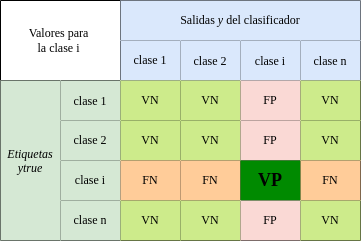
\includegraphics[scale=0.7]{../Figuras/MC_multiple.png}
 \caption{Matriz de confunsión para clasificador multiclases.}
 \label{fig:mcMult} 
\end{figure}

 
 \begin{example}
Tenemos un clasificador encargado de identificar las cinco vocales del español, escritas a mano. Entonces tenemos un total de 5 clases representadas por $a, e, i, o, u$, cada letra representada por un número del 0 al 4. Así la clase $0 = a$, la clase $1 = e$ y así respectivamente. Este fue entrenado con 15 ejemplares etiquetados y se obtuvieron los siguientes resultados:


\begin{center}
\rowcolors{2}{\colTableRow}{white}
\begin{tabular}{c|ccccccccccccccc}

 $Ejemplar$ $e$     & 1 & 2 & 3 & 4 & 5 & 6 & 7 & 8 & 9 & 10 & 11 & 12 & 13 & 14 & 15 \\ \hline
 $Etiqueta $      & a & e & i & o & u & a & a & e & i & i  & o  & u  & o  & u & a \\ \hline
 $Clase$ $y_{true}$ & 0 & 1 & 2 & 3 & 4 & 0 & 0 & 1 & 2 & 2  & 3  & 4  & 3  & 4 & 0 \\ \hline
 $Predicho$ $y$     & 0 & 1 & 3 & 3 & 2 & 1 & 1 & 1 & 2 & 2  & 4  & 4  & 3  & 2 & 0 \\ \hline

\end{tabular}
\end{center}

 Ahora para hacer la matriz de confusión $MC$ notamos que tenemos una matriz de $5 x 5$, donde $MC[i]= Predicho$ y $MC[][j] = EtiquetasReales$. Entonces necesitamos contabilizar las predicciones y asignarlas a sus respectivas celdas, donde con la tabla anterior notamos que en el ejemplar $e3$ con $y_{true}(e3)= 2$, se predijo que $y(e3)=3$, entonces $MC[2][3] +=1$, pues la etiqueta nos posiciona en la fila $2$ y lo predicho en la columna $3$. Ahora en el ejemplar $e4$ con $y_{true}(e4)= 3$ se predijo que $y(e4)= 3$, entonces  $MC[2][2] +=1$. Así con cada ejemplar vamos a ir sumando su clasificación. Para construirla tendríamos un pseudocódigo siguiente:
 \begin{verbatim}
  def getMC (Ejemplares, y):
      """
      :param y:  salidas obtenidas (int)
      """
      MC = [len(y)][len(Ejemplares] # y == Ejemplares
      full_zeros(MC)
      for e in range (0, len(Ejemplares)):
          predicho = y[e]
          y_true = Ejemplares[e].etiqueta
          MC[predicho][y_true] += 1
  retrun MC
 \end{verbatim}

Dados los datos anteriores tenemos, la siguiente matriz de confusión: 
 \begin{table}[H]
\begin{center}
%\rowcolors{2}{\colTableRow}{white}
\begin{tabular}{|c|c|c|c|c|c|c|c|}
\cline{3-7}
\multicolumn{2}{c|}{} & \multicolumn{5}{c|}{Salidas $y$} \\
\cline{3-7}
\multicolumn{2}{c|}{} & 1 & 2 & 3 & 4 & 5 \\
\hline
\multirow{5}{*}{\begin{sideways} Etiquetas~ \end{sideways}} & 1 & $2$ & $2$ & $0$ & $0$ & $0$ \\
\cline{2-7}
& 2 & $0$ & $2$  & $0$ & $0$ & $0$ \\
\cline{2-7}
& 3 & $0$ & $0$  & $2$ & $1$ & $0$ \\
\cline{2-7}
& 4 & $0$ & $0$  & $0$ & $2$ & $1$ \\
\cline{2-7}
& 5 & $0$ & $0$  & $2$ & $0$ & $1$ \\
\hline
\end{tabular}
\end{center}
\caption{MC = Matriz de confusión multiclase.}
\label{Table2}
\end{table}

\label{ej:muticlase}
\end{example}
 

 Para calcular los valores \emph{VP, VN, FP,FN}, por clase se propone el siguiente pseudocódigo:
 \begin{verbatim}
  MC = getMC(y_salidas, y_true)
  
  VP = VN = FP = FN = [0,0,0,0,0]

  for i in range(len(MC)):
    for j in range(len(MC[0])):
        FN[i] = FN[i] + MC[i][j] if (i != j) else FN[i]
        FP[i] = FP[i] + MC[j][i] if (i != j) else FP[i]
        VP[i] = MC[i][j] if (i == j) else VP[i]
    VN[i] = sum(MC) - FN[i] - FP[i] -VP[i]
 \end{verbatim}

 Si quisiéramos saber los valores \emph{VP, VN, FP,FN}, para todo el desempeño total, simplemente sumamos lo obtenido en cada clase así:

 \begin{verbatim}
  VP_total = sum(VP)
  VN_total = sum(VN)
  FP_total = sum(FP)
  FN_total = sum(FN)
 \end{verbatim}

    Ahora los valores de cada celda nos representan lo siguiente:
 
   \begin{itemize}
     \item \emph{$VP_{total}$}, toda la diagonal de la matriz. La salida del modelo coincide con lo etiquetado con el ejemplar.
     \item \emph{$VN_{total}$}, todas las veces que no era la clase i y dijo que no era de la clase i.
     \item \emph{$FN_{total}$}, todas las veces que era $clase_{i}$ y dijo que era $clase_{x}$. (deseado $FN = 0$ )
     \item \emph{$FP_{total}$}, todas las veces que predijo que era $clase_{i}$ y era $clase_{x}$. (deseado $FP = 0$ )
   \end{itemize}
 
    Así que, si los valores que no están en la diagonal de la matriz son cero o todas nuestras clasificaciones están en la diagonal, podemos decir que nuestro modelo aprendió a clasificar correctamente todas las clases.
 
 \end{description}
\begin{description}

 \item [Precisión y recuperación]: 
 La precisión (\emph{precision}) nos dice la proporción de ejemplares que se logró clasificar correctamente. 
 Mientras que recuperación (\emph{recall}) nos dice cuantas asignaciones de lo que nos interesa pudo clasificar correctamente en otras palabras donde del total de las respuestas correctas que se pueden tener, cuantas respuestas positivas acertadas se tuvo.
 
 
    \begin{equation}
        P = \dfrac{VP}{VP + FP}  = \dfrac{Verdaderos Positivos}{Valores Esperados}
    \end{equation}
    \begin{equation}
        R = \dfrac{VP}{VP + FN} = \dfrac{Verdaderos Positivos}{Valores Predichos}
    \end{equation}

    \begin{figure}[H]
        \centering
        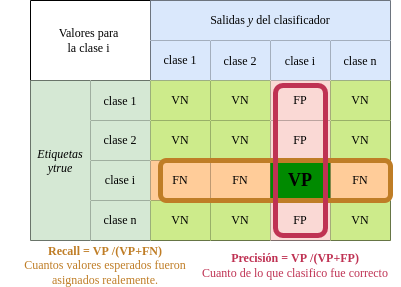
\includegraphics[scale=0.7]{../Figuras/Medidas_pr.png}
        %\caption{Matriz de confunsión para clasificador multiclases.}
     \label{fig:mcPR} 
    \end{figure}

    
    \begin{itemize}
     \item Cuando el modelo detecta los ejemplares, pero los incluye en otras clases también: \emph{P} es bajo y \emph{R} es alto. 
     \item Cuando el modelo no detectó bien los ejemplares, pero tampoco los incluyo en otras clases: \emph{P} es alto y \emph{R} es bajo. 
     \item Cuando el modelo detecta los ejemplares y no los incluye en otras clases:\emph{P} y \emph{R} es alto. 
     \item Cuando el modelo no detecta los ejemplares:\emph{P} y \emph{R} es bajo. 
     \end{itemize}


     En ocasiones le daremos más importancia al recall y en otras a la precisión. Retomando el ejemplo previo \ref{ej:binario}, no nos importa tanto los casos de error tipo 1, donde el modelo se equivoco con los ejemplares negativos, nos importa los errores de tipo 2, los Falsos Negativos, en este caso le tomaremos especial atención al Recall y que este sea alto. Pero si bien nuestra tarea es detectar cuando un correo es spam, no impacta tanto que aunque en ocasiones un correo sea spam, no lo clasifique como tal (error tipo 2 FN), nos es crucial que un correo que no sea spam nos lo clasifique como tal (error tipo 1 FP). Así deseando que los falsos positivos se acerquen a cero, dándonos como resultado una precisión alta aunque el recall sea bajo. 

     
 \item [Exactitud y medida f ]: La exactitud (\emph{accurrancy}) es una medida de cuántas predicciones correctas en total hizo el modelo para el conjunto de datos completo (no se recomienda usar si tienes clases desbalanceadas, es decir, muchos elementos de una clase y poco de otra pues nos puede fallar totalmente con las clases pequeñas y aun así su valor sería alto). La medida f (\emph{(f score)}) se utiliza para combinar las medidas de precisión y recall en un solo valor. Es práctico porque hace más fácil el poder comparar el rendimiento combinado de la precisión y la recall. Se dan las ecuaciones a continuación:
    
    \begin{equation}
     Acurrancy = A = \dfrac{VP+VN}{VP + VN + FP + FN} = \dfrac{VP+VN}{Todos Los Valores Clasificados}     
    \end{equation}

    \begin{equation}
     F = \dfrac{2}{\dfrac{1}{P} +\dfrac{1}{R} }= 2 \dfrac{P * R}{P + R}
    \end{equation}

La medida f, también la podemos escribir (con un poco de aritmética) como:
    \begin{equation}
     F = \dfrac{2VP}{2VP+FP+FN}
    \end{equation}
\end{description}




\chapter{Perceptrón multicapa}
\section{Intro}

Perdí el archivo :CCCC

\section{XOR}


Anteriormente, habíamos logrado separar clases de ejemplares siempre y cuando estos se pudieran modelar en un plano linealmente separable. Hasta ahora había sido un reto importante (no logrado) hacer clasificaciones de ejemplares distribuidos en un plano no separable linealmente, como lo es \emph{la función XOR} donde, tenemos que las respuestas positivas se encuentran en una diagonal opuesta a las respuestas negativas y no hay manera de separar a los blancos de los negros con una sola frontera lineal, lo que hace imposible separar con un solo perceptrón. Entonces notamos que necesitamos de dos líneas que nos permitan separar el plano. Así llegamos a la idea que necesitamos más de una capa, que nos permita hacer la siguiente separación del plano.

\begin{figure}[H]
 \centering
 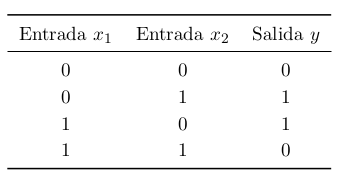
\includegraphics[scale=0.5]{../Figuras/TablaXor.png}
 \caption{Tabla de verdad para la función XOR.}
 \label{fig:tablaXOR}
\end{figure}

\begin{figure}[H]
 \centering
 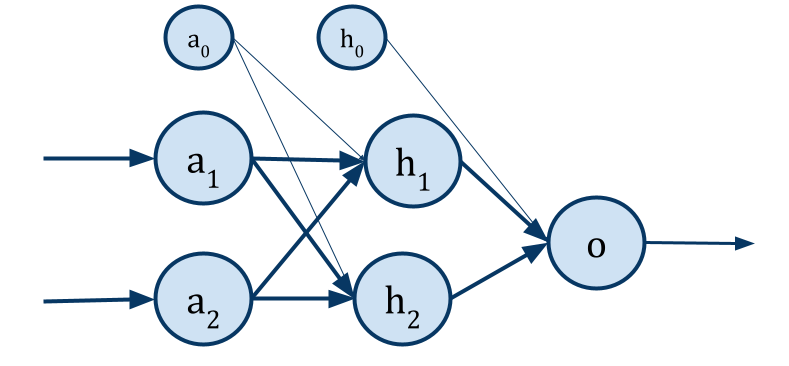
\includegraphics[scale=0.3]{../Figuras/XOr.png}
 \caption{Perceptrón para la función XOR, con una capa oculta.}
 \label{fig:pXor}
\end{figure}



En la tabla de verdad notamos que para la función XOR, cuando la suma de las entradas es:
\begin{itemize}
 \item par (tomando en cuanta al cero como par) la salida es $0$.
 \item impar la salida es $1$.
\end{itemize}


Para poder aprender la función únicamente tenemos que añadir una capa intermedia, la llamada capa oculta. Esta capa será la responsable de tomar las características de los vectores de entrada.


Ahora para la función tenemos dos entradas, una capa oculta (con dos neuronas) y una salida. Las neuronas en la capa oculta nos permitirán dividir el plano. Así, una solución sería que las neuronas ocultas denotadas por $h$ (\emph{hidden} de oculto en inglés) compartan pesos, la primera neurona $h_1$ haría la función $OR$, haciendo la distinción entre las entradas $0 0$, la segunda neurona $h_2$ haría la función $NAND$ haciendo posible distinguir el vector de entrada $1 1$, una vez obtenido estos resultados de la capa oculta la neurona de salida $o$ de output se encargara de distinguir la intersección entra estas, ejecutando la función $AND$. En resumen, la función \emph{XOR} la podemos rescribir como:


\begin{equation}
 \begin{split}
    XOR &= (x_{1} \vee x_{2}) \wedge \neg(x_{1} \wedge x_{2}) \\
    XOR &= AND (OR(x_{1}, x_{2}), NAND(x_{1}, x_{2}))
 \end{split}
\end{equation}

\begin{figure}[H]
 \centering
 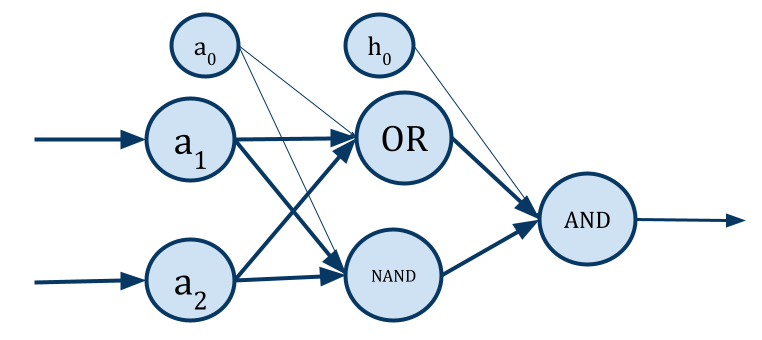
\includegraphics[scale=0.3]{../Figuras/xor.png}
 \caption{Solución para perceptrón de la función XOR.}
 \label{fig:pXorSol}
\end{figure}






\section{Propagación hacia adelante manual}

En está parte vamos a ver como podemos evaluar la red para la solución que se dio en la sección anterior. (Recordemos que tambíen se pueden dar otras soluciones para el XOR).

Entonces el procedimiento matemático general para poder evaluar una red cuando tenemos más de un perceptron. Veamos primero que pasa con el \textbf{xor}, y el \textbf{nand}, por el momento no tomaremos en cuenta las neuronas de entrada $a$ puesto que solo son usadas para almacenar las entradas. La capa oculta está formada realmente por dos percetrones, que dan su salida a una neurona más que es la capa de salida de nuestra red. Para calcular sus salidas debemos aplicar la suma ponderada de las entradas a una función activación, así podemos ver que la salida de una neurona oculta es la siguiente:
 
\begin{equation}
 z_{j} = g (\sum_{i} w_{ij}a_i)
\end{equation}

A estos perceptrones a su vez se le estan aplicando la función de activación sigmoide:

\begin{equation}
 h_{j} = \dfrac{1}{ 1 + e^{-z}}
\end{equation}

Así la neurona de salida recibe a los perceptrones ya evaluados y listos para aplicar pesos a estos y una función de activación, que en este caso son dados de la siguiente forma:

\begin{equation}
 z_{o} = g (\sum_{j} w_{jo}h_j)
\end{equation}

\begin{equation}
 o = \dfrac{1}{1 + e ^{z_o}}
\end{equation}

Así tomando de ejemplo la función XOR, los valores de la capa oculta son evaluados de la siguiente forma, donde $x_{1}$ y $x_{2}$ son evaluados por 0 o 1 según sea necesario:

\begin{equation}
 \begin{split}
 h_{0} &= 1 \\ 
 h_{1} &= g(1w_{01} + x_{1}w_{11} + x_{2}w_{21}) \\
 h_{2} &= g(1w_{02} + x_{1}w_{12} + x_{2}w_{22}) 
 \end{split}
\end{equation}


Entonces hasta aquí ya tenemos los valores de la capa oculta, una vez que ya tenemos este conjunto de valores podemos empezar a trabajar con el tercer perceptor, sus valores de entrada van a estar dados por los valores de activación de $h1$ y $h2$ y por un  sesgo, pues recordemos que es la función $Nand$, por tanto necesitamos movernos ligeramente del origen. Lo que vamos a tener aquí la fórmula se ve similar, lo único  es que ahora los valores de entrada fueron los valores que obtuvimos en el cálculo de la capa anterior:

\begin{equation}
  o = g( h_{0}w{0o} + h_{1}w_{1o} + h_{2}w_{2o})
\end{equation}

Como estamos trabajando capa por capa, primero entran los valores con los que van a trabajar todos los perceptrones, después calculamos todos los de la capa oculta que son independientes entre sí, aunque tengan en común las mismas entradas y finalmente hacemos el cálculo de la siguiente capa, que en ese caso es la se salida, pero bien podría ser otra oculta. 

Por la forma de recorrer la red (de izquierda a derecha) esté algortimo obtiene su nombre de \emph{propagación hacia adelante}, pues lo calculado en la neurona de la capa anterior se propaga directamente a la siguiente capa, en íngles se conoce como \textit{feedfordward}. Cuando tenemos la evaluación de las capas ocultas, podemos obtener finalmente la salida final, con una evaluación final.

Si bien está forma de evalución nos lleva al resultado correcto, este metodo se puede simplificar sobretodo en el caso que estemos manejando más entradas y más perceptrones en las capas ocultas. Así nos daremos cuenta que es posible usar matrices, esta forma de evaluación la veremos en la siguiente sección.

\section{Propagación hacia adelante vectorizada (con matrices)}

 La sección anterior si bien nos da la idea somera de como van a ser las operaciones para el aprendizaje ahora veamos lo de forma matricial. Esto nos ayudará a en un momento dado escrbirlo en el lenguaje de nuestra convencia.
 
 
 Retomamando la red neuronal de la sección anterior ahora con pesos.
 
 \begin{figure}[H]
 \centering
 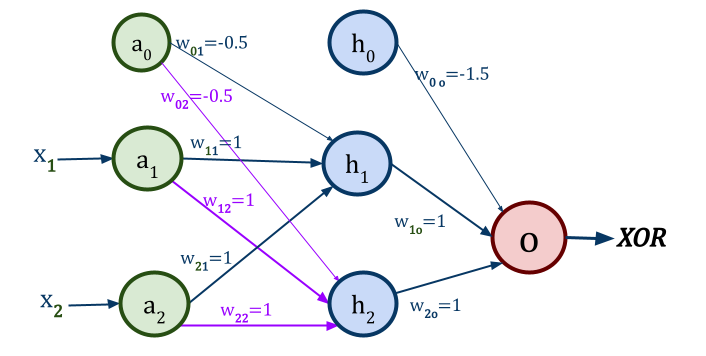
\includegraphics[scale=0.5]{../Figuras/XOR_pesos.png}
 \caption{Función XOR, con capa oculta}
 \label{fig:xorPesos}
\end{figure}

Ahora veamos a las entradas como un vector de la siguiente forma:
 $$
 A =
 \begin{bmatrix}
  a_{0}\\
  a_{1}\\
  a_{2}\\
 \end{bmatrix}
 =
 \begin{bmatrix}
  1\\
  0\\
  1\\
 \end{bmatrix}
 $$
 
 Ahora para poder hacer los siguientes cálculos acomodamos los pesos correspondientes a cada perceptron. Para el primer perceptron tomamos los pesos que están conectados desde la neurona de origen $a_{0}, a_{1}$ y $a_{2}$ hacia la neurona oculta $h_{1}$ (los indices de los pesos indican, el origen y el destino, en ese orden), los colocamos en un renglón de la matriz de pesos, así representamos nuestro primer perceptrón y hacemos lo mismo para $h_{2}$, así obtenemos la siguiente matriz de pesos:
 $$
 W =
 \begin{bmatrix}
  w_{01} & w_{11} & w_{21}  \\
  w_{02} & w_{12} & w_{22}\\
 \end{bmatrix}
 =
 \begin{bmatrix}
  -0.5 & 1 & 1\\
  1.5 & -1 & -1\\
 \end{bmatrix}
 $$
 
 Ya que tenemos la representación de las entradas y pesos en vactores podemos hacer la representación de la activación de estas neuronas de la capa oculta, que es de la forma $H = g(W * A)$, que de forma matricial lo podemos ecribir de la siguiente forma:
 $$
 H=
 \begin{bmatrix}
  h{1}  \\
  h{2}\\
 \end{bmatrix}
 = g \left(
 \begin{bmatrix}
  -0.5 & 1 & 1\\
  1.5 & -1 & -1\\
 \end{bmatrix}
 \begin{bmatrix}
  1 \\
  0 \\
  1 \\
 \end{bmatrix}
 \right) = g \left(
 \begin{bmatrix}
  0.5 \\
  0.5 \\
 \end{bmatrix}
\right) =
 \begin{bmatrix}
  1 \\
  1 \\
 \end{bmatrix}
$$
 
 La matriz resultante representa los valores de activación resultantes en cada perceptrón, el primer valor de la matriz representa el resultado de la activación de $h1$ y el segundo a $h2$. Así ahora tenemos al vector $H$ que sera el vector de entrada para la neurona de salida $o$, procedemos de la misma forma tomando en cuenta al sesgo $h_0$ y a los pesos en forma matricial, nos queda de la siguiente forma $o = g(W_{ho} * H)$:
 $$
 o =
 g \left(
 \begin{bmatrix}
  -1.5 & 1 & 1\\
 \end{bmatrix}
 \begin{bmatrix}
  1 \\
  1 \\
  1 \\
 \end{bmatrix}
 \right) = g \left(
 \begin{bmatrix}
  0.5 \\
 \end{bmatrix}
\right) =
 \begin{bmatrix}
  1 \\
 \end{bmatrix}
 $$
 
 
Hasta este momento ya logramos resolver la función XOR para una sola entrada, esta forma de resolver una red la llamaremos convención 1.
Si queremos que nos de la resupuesta a varias entradas al mismo tiempo tendríamos que modificar un poco la representación de nuestros valores, trasnpodiendo las matrices anteriores que teniamos. Que se verían de la siguiente forma:

 $$
 A^ {T} =
 \begin{bmatrix}
  a_{0} & a_{1} & a_{2}\\
 \end{bmatrix}
 =
 \begin{bmatrix}
  1 & 0 & 1 \\
 \end{bmatrix}
 $$

 $$
 W^ {T}  =
 \begin{bmatrix}
  w_{01} & w_{02}\\
  w_{11} & w_{12}\\
  w_{21} & w_{22}\\
 \end{bmatrix}
 =
 \begin{bmatrix}
  -0.5 & 1.5\\
  1 & -1\\
  1 & -1\\
 \end{bmatrix}
 $$

 $$
 H = g(A^{T}*W^{T}) \\
 $$

  $$
 H=
 \begin{bmatrix}
  h{1} & h{2}\\
 \end{bmatrix}
 = g \left(
 \begin{bmatrix}
  1 & 0 & 1\\
 \end{bmatrix}
 \begin{bmatrix}
  -0.5 & 1.5\\
  1 & -1\\
  1 & -1\\
 \end{bmatrix}
 \right) = g \left(
 \begin{bmatrix}
  0.5 &  0.5 \\
 \end{bmatrix}
\right) =
 \begin{bmatrix}
  1 &  1 \\
 \end{bmatrix}
$$

$$
 o =
 g \left(
 \begin{bmatrix}
  1 & 1 & 1\\
 \end{bmatrix}
 \begin{bmatrix}
  -1.5 \\
  1 \\
  1 \\
 \end{bmatrix}
 \right) = g \left(
 \begin{bmatrix}
  0.5 \\
 \end{bmatrix}
\right) =
 \begin{bmatrix}
  1 \\
 \end{bmatrix}
 $$
 
 
Esta forma se llama la convención 2, lo que estamos haciendo en la convención 2 es más bien poner nuestro ejemplar de manera horizontal. Así cada renglón de $A$ va a representar una entrada el primer valor de cada renglón siempre será el sesgo.
 Así al tener varias entradas de la siguiente forma:
 
 $$
 X =
 \begin{bmatrix}
  0 & 0 & 1 & 1\\
  0 & 1 & 0 & 1\\
 \end{bmatrix}
 $$
 
 A la matriz $A$ es $X$ transpuesta y le agregamos los sesgos, quedando así:
 $$
 A =
 \begin{bmatrix}
  1 & 0 & 0\\
  1 & 0 & 1\\
  1 & 1 & 0\\
  1 & 1 & 1\\
 \end{bmatrix}
 $$
 
 La capa oculta quedaría de la siguiente forma $H = g(W^{T}A)$

 $$
   H
 = g \left(
 \begin{bmatrix}
  1 & 0 & 0\\
  1 & 0 & 1\\
  1 & 1 & 0\\
  1 & 1 & 1\\
 \end{bmatrix} 
 \begin{bmatrix}
  -0.5 & 1.5\\
  1 & -1\\
  1 & -1\\
 \end{bmatrix}
 \right) = g \left(
 \begin{bmatrix}
  -0.5 &  1.5 \\
  0.5 &  0.5 \\
  0.5 &  0.5 \\
  1.5 &  -0.5 \\
 \end{bmatrix}
\right) =
 \begin{bmatrix}
  0 &  1 \\
  1 &  1 \\
  1 &  1 \\
  1 &  0 \\
 \end{bmatrix}
$$

 El resultado de esta matriz $H$ es que, la primera columna está representando la neurona que evalua la función OR y la segunda columna representa el NAND. Para obtener la salida de la neurona $o$ que es un AND, hariamos las mismas operaciones anteriores solo que con sus respectivos pesos y valores de $H^{T}$, así obteniendo lo siguiente $o = g(H^{'}W^{T}) = XOR$:
 
 $$
 o =
 g \left(
 \begin{bmatrix}
  1 & 0 & 1 \\
  1 & 1 & 1 \\
  1 & 1 & 1 \\ 
  1 & 1 & 0\\
  \end{bmatrix}
 \begin{bmatrix}
  -1.5 \\
  1 \\
  1 \\
 \end{bmatrix}
  \right) = g \left(
 \begin{bmatrix}
  -0.5 \\
  0.5 \\
  0.5 \\
  -0.5 \\
 \end{bmatrix}
\right) =
 \begin{bmatrix}
  0 \\
  1 \\
  1 \\
  0 \\
 \end{bmatrix}
 $$


Más adelante esta representación, nos ayudará cuando estemos trabajando con redes neuronales que necesiten \emph{diferentes tipos de características}, como; edades, número de hijos, tamaño de una casa, etc. 
 Esta anotación es mucho más visual para la forma en que vamos a recibir la información (tabla de datos), por eso es más usada está versión.

%Propagación hacia adelante vectorizada (con matrices)
\section{Interpretación matemática del mapeo no lineal}
En esta sección vamos a ver por qué agregar una capa más nos permite calcular funciones que no era posible calcular antes es decir no basta con tener más percepciones en realidad necesitamos tener percepciones que reciban como entrada la salida de percepciones anteriores y esto lo vamos a notar aquí por eso el selector es una función tan útil para poder explicar estos conceptos de entrada que teníamos al inicio de la función sort eran los valores 0 0 0 1 1 0 y 1 1 estos solamente los podría bueno puede utilizar perceptor únicamente para evaluar funciones que sean linealmente separables entonces cuando hemos aplicado la primera capa donde pudimos poner tantas operaciones como que hicimos lo que hicimos fue tomar estas entradas y mapear las a un conjunto distinto y esté ocurriendo en este nuevo conjunto 

Observen que las entradas ahora son 01 11 11 10 es decir estas dos están duplicadas ya no tengo el 0 0 por eso es que se dice que trabajamos con un mapeo no lineal nuestra función sigmoide o nuestra función escalón transformaron nuestro espacio de manera que no tenemos ahora una relación 1 a 1 qué efecto va a tener. Aquí tenemos una vez más cuáles son las entradas originales las entradas que se obtuvieron es bueno salidas de las capas ocultas que van a hacer ahora las entradas para el último perceptor entonces veamos acá qué pasó con este cuadro aquí teníamos cuatro datos que no eran linealmente separables después de la primera capa fue como haberlo plegado a otro espacio de dos dimensiones, pero observen ahora que como que esto es bueno vamos a ver quién se mató a quién el 0 0 se convirtió en 0,1 es decir este para acá el 0,1 se convirtió en 1,1 este fue para acá el 1010 también se convirtió en 1,1 es otro de acá y el 11 se convirtió en el 10 está aquí entonces nuestros puntos negros como que giraron un poquito y quedaron aquí y nuestros dos puntos blancos quedaron mapeados uno encima del otro en el mismo punto de este lado. 

Entonces ahora sí lo puedo separar con un plano qué pasa en medio de los dos cualquiera que lo logre es bueno entonces estos tres valores quedaron mapeados ahora a un nuevo espacio que por cierto tiene una dimensión solo hay un valor. Entonces el paso fundamental radicó en que pudimos mapear este espacio hacia un espacio nuevo donde si es posible separar a nuestros datos linealmente y sobre esto pues ya simplemente aplicamos lo que podía hacer cualquier perceptual matemáticamente ese es el poder que nos está añadiendo una capa de en medio y básicamente lo podemos generalizar ahora si a cualquier función. Es posible quitar los sesgos si utilizamos la función escalón como función de activación y definimos precisamente el menor o igual para la parte del escalón en esta ocasión vamos a obtener valores que están exactamente en este punto de salto así es que vamos a tener que decir quién queda a la izquierda quien quiere a la derecha y entonces podemos hacer esto igual se necesitan dos capas, pero podemos quitarnos la parte de los sesgos porque nuestras fronteras si están pasando por ser un coma se hace solo por curiosidad bien aquí tenemos entonces ya esa interpretación vemos que los ceros negativos se van a tomar como ceros y solamente los positivos van a quedar como unos y automáticamente se puede hacer esta versión resumida. 


 %Interpretación matemática del mapeo no lineal
\section{Propagación hacia adelante para el perceptrón multicapa}

Ahora para el modelo de una red en general tenemos nuestra arquitectura base que va a ser una red en capas también se le conoce como el perceptron multicapa (tipo feed-forward) en esta primera versión tenemos la capa de entrada que realmente solo recibe las entradas y el sesgo. Las salidas de cada capa sirven de entradas a la capa inmediatamente posterior en la red multicapa. Por lo general todas las salidas de una capa se distribuyen a todas las neuronas de la siguiente capa, formando capas completamente conectadas (fully-connected layers).
Cuando la red multicapa incluye más de una capa oculta, se dice que la red neuronal es profunda [deep neural network].
Los niveles de actividad de las neuronas de cada capa vienen dados por una función de activación no lineal de los niveles de actividad de las neuronas de la capa inferior.

(Insertar imagen de red).

Anteriormente habiamos estado asignando pesos a ojo/intuición, esto porque eran pocos los valores de entrada, esto normalmente no es así y vamos a desconocer en la totalidad los pesos necesarios que se aproximen a nuestra función objetivo.  

La red neuronal es en sí, es una función que nos va permitir pasar un vector de n dimesiones a uno de m dimensiones, con n la cantidad de características en nuestros datos y m la cantidad de características que necesitamos obtener.  

Entonces vamos a utilizar un tipo de codificación que se utiliza para la clasificación, llamado One-hot encoding, donde nos vamos a enforcar en el valor más elevado en nuestros resultados. Ahora nuestros problemas involuran más de dos clases, donde cada renglón de nuestra matriz de salida nos va indicar si pertence o no a una clase, algun ejemplar dado. Así tenemos cada dimensión en la matriz va a representar una clasificación, por ejemplo si queremos distinguier en una imagen entre un coche, casa, animal lo podríamos codificar de la siuiente forma:

$$
Salida 1 = coche =
\begin{bmatrix}
  1 & 0 & 0 \\
  \end{bmatrix}
\begin{bmatrix}
  1 \\ 
  0\\ 
  0 \\
  \end{bmatrix}
$$

$$
Salida 2 = casa =
\begin{bmatrix}
  0 & 1 & 0 \\
  \end{bmatrix}
\begin{bmatrix}
  0 \\
  1 \\
  0 \\
  \end{bmatrix}
$$
$$
Salida 3 = vaca =
\begin{bmatrix}
  0 & 0 & 1 \\
  \end{bmatrix}
\begin{bmatrix}
  0 \\ 
  0 \\ 
  1 \\
  \end{bmatrix}
$$

Toda la parte del aprendizaje, de reconocer distintos patrones, obtención de características varias, va a quedar entre \emph{la capa de entrada y las capas ocultas}, para que al final nos quedemos únicamente con el problema de separar las clases unas de otras tantas sean necesarias, \emph{en la capa de salida} y tengamos nuestra información clasificada. Así cada neurona de salida es una clase, especifica, entonces si se activo esa neurona nos indica que nuestro ejemplar pertence a dicha clase. Es importante no escatimar en el número de perceptrones necesarios para la clasificación a la salida, pues esto podría resultar en asignación conjunta de características, que se podrían interpretar como similitudes entre clases y en caso de no existir, dificultaarian enormemente la distinción entre características y generar fallos a la red. Siempre asignar tantas dimenciones de salida (perceptrones) como clases.

Los calculos para cada capa intermedia realmente son las mismas que hemos visto anteriormente representandose de la siguiente forma:
\begin{equation}
 a_{j}^{(l+1)} = g \left( \sum_{i} w_{ij}^{(l)}a_{i}^{(l)} \right)
\end{equation}

Con $l+1$ representando el número de capa a la que vamos, $g$ la función activación (normalmente podemos usar la función sigmoide) y $a_i$ los valores de las entradas. 


 %Propagación hacia adelante para el perceptrón multicapa

%%
\chapter{Entrenamiento por retropropagación}

\section{Esquema general entrenamiento}
 
 En este capítulo vamos a trabajar con el entrenamiento (específicamente por retropropagación), en esta sección abordaremos primero el esquema general del entrenamiento. 
 A lo largo del capítulo veremos la derivación del primer algoritmo de entrenamiento para perceptrones multicapa (este es de los más comunes en esta área y el primero descrito propiamente).

En el tercer capítulo habíamos visto el concepto de aprendizaje para una máquina, ahora vamos a definir en que consiste aprender algo en el campo de las redes neuronales. Retomando lo descrito en ese capítulo, recordemos que aprender para un modelo es más que nada encontrar una función que se asemeje a ciertas salidas específicas, está función está dentro de un espacio de funciones posibles propuestas. La función que deseamos encontrar modela algún tipo de tarea que nos interesa que se aprenda. 

\begin{definition}
 \textbf{El problema de aprendizaje para un perceptrón multicapa:} Dada una arquitectura de red neuronal, encontrar los pesos tales que la función $h\Theta(\vec{x}) $ (definida por la red neuronal) aproxime, hasta cierta tolerancia, la función de interés $ f(\vec{x})$. \\ Con $\vec{x}$ los datos de entrada.
 
\end{definition}

En la definición anterior, el vector $\vec{x}$, consisten en distintas características de los ejemplares provistos, según sea el problema a resolver, por ejemplo:
\begin{itemize}
 \item Segmentos de alguna canción.
 \item Píxeles de imágenes.
 \item Valores equivalentes a precios del mercado.
\end{itemize}

En este momento nos estamos concentrando en problemas de clasificación así que estás redes estan clasificando los ejemplares según ciertas características. Estas clasificaciones pueden ser muy interesantes, algunas por ejemplo se pueden dedicar a clasificar canciones, identificando ciertas emociones que transmiten como tristeza o alegria. 

Nuestra red neuronal va empezar sus calculos apartir de los datos de entrada $\vec{x}$, entonces al finalizar cada uno de los ejemplares va a ser mapeado a alguna clase (en el espacio de clases). Por medio de una función donde $f(x)$ es nuestra función ideal que hacer el mapeo exacto los ejemplares a su clase. Así si logramos que nuestra función $h\Theta(\vec{x})$ se aproxime a $f(x)$, la red neuronal nos daría las respuestas esperadas dado ciertos ejemplares, como por ejemplo:
\begin{itemize}
 \item Dado unas imagenes de distintas plantas, identificar correctamente el nombre de cada una.
 \item Dado una fragmento de canción indicarnos su genero.
 \item Dada una oración identificar si contiene un mensaje de odio.
\end{itemize}

Entonces el reto de la red neuronal es aproximar una función $f(x)$ (que se asume existe en el universo),
primero debemos intentar calcular $h\Theta(\vec{x})$ (\emph{h} de hipótesis, de un espacio de hipótesis). Está hipotesis puede que aproxime muy bien la función pero en la mayoria de los casos no es así, entonces iremos haciendo ajustes a los pesos (que definen la función h) para que pueda aproximarse lo más posible a nuestra función objetivo.


Como en muchos casos vamos a intentar aproximar funciones que no corresponden a un concepto matemático, sino más a percepciones humanos tales como sentimientos o clasificar abstraciones humanas, entonces se puede dar el caso que realemente no se pueda aproximar con total exactitud la función y le demos un cierto \emph{grado de tolerancia}, donde se asume que se pueda dar ciertos errores en ciertos ejemplares. Dependiendo del contexto vamos a asignar el rango de tolerancia de errores.

Es importante notar que si los datos de entrenamiento resultan clasificados con mucha precisión es probable que la red este aprendiendo datos no utiles para la tarea dada, es decir ese aprendiendo \emph{ruido}. Y al momento pasar los ejemplares de prueba no entregue buenos restultados.

Eentrenar una red para que se aproxime a la función objetivo cada vez más, debemos hacer lo siguiente:
\begin{itemize}
 \item  Definir una \emph{función de error} o pérdida $J$ (o $L$ de lost, perdida en íngles) que mida la distancia entre los valores deseados y los valores obtenidos con un conjunto de pesos dados $\Theta$ .
 \item Utilizar alguna \emph{técnica de optimización} de funciones que minimize este error.
 \item Definir la \emph{arquitectura} de la red, la \emph{función de error} y la técnica de
optimización, conciderando el tipo de función objetivo.
\end{itemize}

Una vez que ya sabemos en que consiste el entrenamiendo veamos un esquema general conocido como \emph{entranamiento por retropropagación} o propagación hacia atras, en íngles \textit{Backpropagation}. Anteriormente habíamos visto la evalución de una red con propagación hacia delante (de izquierda a derecha), con la retroprogación vamos a recorrer la red hacia atras (de derecha a izquierda), de la siguiente forma:
\begin{itemize}
 \item Utilizar \emph{la regla de la cadena} para obtener el gradiente de la función de error con
respecto al conjunto de pesos, dado un conjunto de datos de entrenamiento \emph{$X$} con sus etiquetas \emph{$Y$}.
\item Utilizar \emph{descenso por el gradiente} para encontrar un mínimo, lo suficientemente
bueno, de la función de error. Está técnica es la más sencilla, por eso usualmente se utilizaba en un principio
\begin{itemize}
 \item La idea es que al inicio no sabemos cuánto deben de valer los pesos para modelar correctamente la función, entonces 
 al comienzo se hace una asignación aleatoria de pesos. Existe un conjunto de pesos ideales a los cuales queremos aproximar nuestros pesos aleatorios. Con estos calculamos el error que tiene nuestros pesos, haciendo las comparaciones con los datos que se obtuvieron al aplicar el feedforward, sobre los datos de entrada con los datos esperados. El desenso por el gradiente va modificar poco a poco los pesos, para tengamos una nueva (y mejor) aproximación y nos acerquemos más a una región donde el error sea menor.
 Para calcular el descenso por el gradiente, se calculan las derivadas de la función de error con respecto a los parámetros. 
 \item Entonces tenemos una actualización de la siguiente forma: 
    \begin{equation}
     Theta' = Theta - \alpha \nabla_{\Theta}J
    \end{equation}
        Donde \emph{Theta} es la propuesta para nuestros parametros iniciales, $\nabla_{\Theta}$ es el gradiente que nos da el máximo acenso de la función de error, el cúal lo invertimos con el menos, para que siempre nos dirijamos al minimo local más proximo.  
\end{itemize}

\item Se puede usar otra técnica de optimización más avanzada, pero esta también involucraría al grandiente. 

\item La derivación original utilizaba diferencias al cuadrado como función de error. Esta la pueden consultar en 
Russell, Stuart y Peter Norving (2010). Artificial Intelligence, A Modern Approachs.

\item Para problemas de clasificación es más efectivo usar entropía cruzada como método de optimización. Para problemas de regresión es adecuado usar diferencias al cuadrado.
\end{itemize}

\section{Función de error: Entropía cruzada}
En está sección veremos una de las funciones de error más utilizadas en el campo de redes neurnales, usada sobre todo en problemas de clasificación, la entropía cruzada (en inglés \emph{cross entropy}) la cual tiene su origen en el área de la teoría de la información, la cual mide: \textbf{la cantidad de bits necesarios para identificar una clase} dada la hipótesis de la red representada como $h\Theta (\vec{x}) $, que trata de asemejar la función objetivo $y(\vec{x})$, la cúal es la que tiene los valores reales asociados a las etiquetas.

Uno de los labores de la red neuronal es codificar con \emph{bits} la información que recibe para hacer asignaciónes de la características encontradas y así clasificarlos. Todo el tiempo se está intentando predecir si la función propuesta se asemeja lo suficiente a la función objetivo, en caso de ser así ser podrá codificar adecuadamente nuestros ejemplares.

La formula de entropía cruzada usada en este texto será la siguiente:
 \begin{equation}
  J (\Theta) = -\dfrac{1}{m}\left[\sum_{i=1}^{m}\sum_{k=1}^{s_{L}}y_{k}^{i} log( h_{\Theta}(x^i))_{k}+(1-y_{k}^{i})log(1- h_{\Theta}(x^i))_{k}  \right]  
  \label{entropiaCruzada}
 \end{equation}

 donde:
 \begin{itemize}
  \item \emph{m} es el número de ejemplares del entrenamiento.
  \item \emph{$s_{L}$} es el número de neuronas en la capa L .
  \item \emph{$y_{k}$} es el valor para la k-ésima neurona de salida y toma valores en {0,1}.

 \end{itemize}
  
En la primera parte notamos que tenemos una fracción, está es en esencia la que nos da el promedio de error de la red sobre el número de ejemplares de entrenamiento evaluados en ese momento (m). Seguido de una multiplicación de la suma de los ejemplares que nos da todas las contribuciones de error, que está a su vez contine la suma de las neuronas en la capa de salida de las neurnonas de cada clase. Así en está suma podemos distinguir dos partes, la primera es una multiplicación que compone de la etiqueta real asociada al ejemplar multiplicado por el logaritmo de la etiqueta asignada por la red, y la segunda parte de una multiplicación de uno menos la etiqueta real por el log de uno menos lo dado por la red. Así en está parte se está tomando en cuenta las dos posibilidades que puede tomar cada neurona de salida respecto al ejemplar dado, $0$ no pertenece a la clase y $1$ pertenece a la clase. 

En el primer caso $y_{k}$ toma el valor de cero, entonces la primera parte de está sección se va también a cero, es ahí donde la segunda parte nos permite evaluar que tan lejos estuvimos de la respuesta correcta usando el logaritmo de está. Ahora supongamos que lo deseado era que la neurona predijo $1$ pero lo correcto era $0$, la primera parte se va a cero y en la segunda parte tendrémos un logaritmo de un número cercano a cero dandonos que nos vamos a acercar a menos infinito, es por eso importante el signo negativo en la parte inicial de la función, pues nos va ayudar a que la función nos indique a infinito cuando estamos errados en el resultado.

Ahora en caso de obtener la respuesta deseada, con una salida de $0$ cuando en efecto era este, entonces tendremos el $log(1)$ que es cero, así nuestra función de error valdrá $0$, este caso es poco común pues recodemos que para función de activación $h_{\Theta}$ usando la función logística solo se acerca al $1$. El caso que lo deseado era que nos diera $1$ la neurona esta contemplado en la primera parte donde de nuevo con la ayuda del logaritmo en caso de dar la respuesta incorrecta $0$ este apuntara hacía menos infinito y con ayuda del menos de afuera va hacía infinito, y en caso de estar en lo correcto nos vamos a acercar al cero, dandonos como resultado un error cercano a cero. 

En resumen con esta función si estamos en lo correcto vamos a acercarnos a cero, de lo contrario va a tener hacia infinito.


\section{Derivada de la función logística}

Para poder calcular el gradiente, primero debemos ver la derivada de la función logística. Recordemos en la siguiente figura 
como se ve la función logística.

\begin{figure}[h]
 \centering
 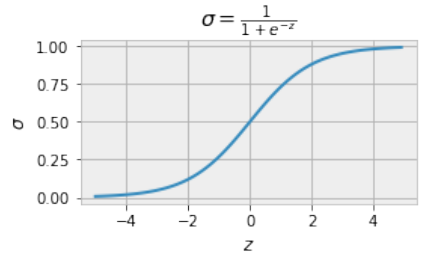
\includegraphics[scale=0.5]{../Figuras/devLog1.png}
 \caption{Gráfica función logistica.}
 \label{fig:graficaLog1}
\end{figure}
\begin{figure}[h]
    \centering
    \subfloat[Función logistica.]{
            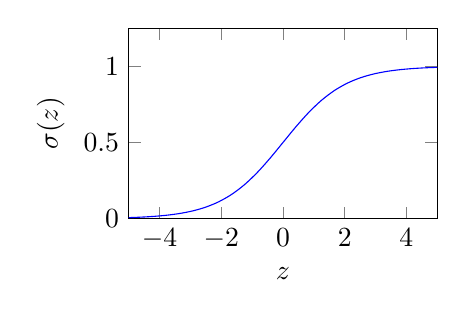
\begin{tikzpicture}
            \begin{axis}[width=5.5cm,height=4cm,ylabel=$\sigma(z)$,xlabel=$z$,ymin=0,ymax=1.25,xmin=-5,xmax=5]
                \addplot[blue,smooth] {1/(1+exp(-x))};
                %\addlegendentry{$y = \dfrac{1}{1+e^{-x}}$}
            \end{axis}
        \end{tikzpicture}
    }
        \caption[Funciones de activación]{}
        \label{fig:sigmoid-tanh}
\end{figure}


La función logistica estandar centrada en el origen como en la figura \ref{fig:graficaLog1} se escribe de la siguiente forma:
\begin{equation}
 \sigma(z) = \dfrac{1}{1+e^{-(z)}}
\end{equation}

Los siguientes calculos son realizados para un solo perceptrón, en concreto uno de salida, donde este está recibiendo los datos de salida de neuronas en la capa oculta, así el factor $z$ que está recibiendo la función, es la combinación lineal de los valores de entrada multiplicados por los pesos asignados para esté perceptrón y sumados todos. Entonces $z = X\Theta = [X_0\theta_0 +X_1\theta_1+...+X_n\theta_n]$. Así nuestra función queda de la siguiente forma:

\begin{equation}
  \sigma_{\Theta}(X) = \dfrac{1}{1+e^{-X\Theta}}
\end{equation}

Entonces vamos a calcular la derivada de esta función con respecto a cualquiera de estos parámetros $i$ de $z$.
Por la regla de la cadena comenzamos calculando la derivada queda de la siguiete forma:

\begin{equation}
 \dfrac{\partial\sigma}{\partial\theta_{i}}= -\dfrac{1}{(1-e^{-X\Theta})^2}e^{-x\Theta}(-x_{i})
\end{equation}

Reescribiendo la misma derivada con un poco de algebra nos queda de la siguiete forma:
\begin{equation}
 \dfrac{\partial\sigma}{\partial\theta_{i}}= \dfrac{1}{1+e^{-X\Theta}}  \dfrac{e^{-x\Theta}}{1+e^{x\Theta}} x_{i}
\end{equation}

Con la reescritura anterior nos damos cuenta que tenemos la función sigma en uno de los productos así que procedemos a sustituirlo y a sumar y restar unos unos. Así obteniendo lo siguiente:
\begin{equation}
 \dfrac{\partial\sigma}{\partial\theta_{i}}= \sigma_{\Theta}(X)\dfrac{e^{-x\Theta}-1+1}{1+e^{x\Theta}} x_{i}
\end{equation}

Vamos a separar a conveniencia los terminos de la siguiente forma:
\begin{equation}
 \dfrac{\partial\sigma}{\partial\theta_{i}}= \sigma_{\Theta}(X)
 \left( \dfrac{1+e^{-x\Theta}}{1+e^{-x\Theta}}-\dfrac{1}{1+e^{-x\Theta}}\right)x_{i}
\end{equation}

Así sustituyendo con la función sigmoide y llevando a uno, llegamos a lo siguiente:
\begin{equation}
 \dfrac{\partial\sigma}{\partial\theta_{i}}= \sigma_{\Theta}(X)
 (1- \sigma_{\Theta}(X))x_{i}
\end{equation}

Entonces lo que tenemos es una propiedad bastante interesante de la función logística. Se está calculando la derivada de sigma con respecto al exponente osea que sería:
Entonces lo que vemos es que la derivada de la sigmoide es la sigmoide por uno menos la sigmoide:

\begin{equation}
 \dfrac{\partial\sigma}{\partial\theta_{z}}= \sigma(1- \sigma)
\end{equation}


\begin{figure}[H]
 \centering
 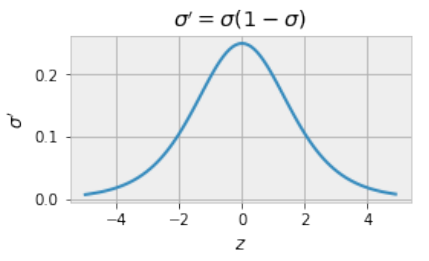
\includegraphics[scale=0.5]{../Figuras/devLog.png}
 \caption{Gráfica de la derivada de la función logistica.}
 \label{fig:graficaLogDev}
\end{figure}

Las funciones logísticas se utilizan a menudo en redes neuronales para introducir no linealidad en el modelo o para sujetar señales dentro de un intervalo específico . Un elemento de red neuronal popular calcula una combinación lineal de sus señales de entrada y aplica una función logística limitada como función de activación al resultado; este modelo puede verse como una variante "suavizada" de la neurona umbral clásica .

Estas relaciones dan como resultado implementaciones simplificadas de redes neuronales artificiales con neuronas artificiales. Las funciones sigmoidales que son antisimétricas con respecto al origen (por ejemplo, la tangente hiperbólica) conducen a una convergencia más rápida cuando se entrenan redes con retropropagación.

Una opción común para la activación o "aplastamiento" funciones, usadas para grandes magnitudes para mantener la respuesta de la red neuronal limitada. 

Las funciones logísticas se utilizan en varios roles en estadística. Por ejemplo, son la función de distribución acumulativa de la familia logística de distribuciones y, un poco simplificadas, se utilizan para modelar la posibilidad que tiene un jugador de ajedrez de vencer a su oponente en el sistema de clasificación.

En la siguiente sección veremos la derivada de la función de error.

\input{secciones/EntrenamientoRetropropagacion/04Parcial con respecto a los pesos en la última capa}
\input{secciones/EntrenamientoRetropropagacion/05Parcial con respecto a los pesos en la penúltima capa}
\input{secciones/EntrenamientoRetropropagacion/06Vectorización}

\chapter{Optimización del entrenamiento} 
\section{Problemas en redes profundas}

Hasta este momento ya se ha visto como modelar desde una neurona hasta una red neuronal propiamente, se ha visto como hacer la configuración de tal manera que nos clasifique ejemplares, así como detectar el error en los pesos asignados y ajustarlo para mejores resultados. Ahora al momento de modelar redes neuronales profundas (en inglés deep neuronal networks, \emph{DNN}) tenemos que aceptar que el cálculo de estás asignaciones y ajustes requieren tiempo de cálculo, así llegando al \emph{primer problema, el tiempo de computación}. Y ademas nos podemos encontrar con \emph{el problema del sobreaprendizaje} este aparece cuando tenemos demasiadas hipótesis válidas pero no de suficientes datos para poder descartar todas menos la correcta. 

Cuando ajustamos los parámetros de una red neuronal a los datos del conjunto de entrenamiento, no podemos diferenciar las características realmente útiles de las irrelevantes o de las debidas al muestreo del conjunto de entrenamiento, por lo que siempre estamos
expuestos al riesgo de sobreajuste (overfitting en inglés).


 Métodos de regularización o la disminución de pesos  o la dispersión, se puede aplicar durante el entrenamiento para combatir el sobreajuste. Alternativamente, la regularización de dropout, omite aleatoriamente neuronas de las capas ocultas durante el entrenamiento. . Finalmente, los datos se pueden aumentar a través de métodos como el recorte y la rotación, de modo que los conjuntos de entrenamiento más pequeños se pueden aumentar de tamaño para reducir las posibilidades de sobreajuste.

Las DNN deben considerar muchos parámetros de entrenamiento, como el tamaño (número de capas y número de unidades por capa), la tasa de aprendizaje y los pesos iniciales. El barrido a través del espacio de parámetros para obtener parámetros óptimos puede no ser factible debido al costo en tiempo y recursos computacionales. Varios trucos, como el procesamiento por lotes (calcular el gradiente en varios ejemplos de entrenamiento a la vez en lugar de ejemplos individuales)  aceleran el cálculo, lo veremos más adelante. Las grandes capacidades de procesamiento de las arquitecturas de muchos núcleos (como GPU) han producido aceleraciones significativas en el entrenamiento.

Para mayor información del tema se sugiere leer el siguiente enlace:

CHAPTER 5 Why are deep neural networks hard to train? \url{http://neuralnetworksanddeeplearning.com/chap5.html}

El siguiente enlace les puede ayudar a ver como cada hiperparemetro puede afectar a los resultados de la red neuronal.
\url{https://quetzalcoatl.fciencias.unam.mx/moodle/mod/url/view.php?id=634&redirect=1}

Para ayudarnos a los calculos con el gradiente vea los siguientes enlaces:
\begin{itemize}
 \item \url{https://youtu.be/nUUqwaxLnWs}
 \item \url{https://youtu.be/FDCfw-YqWTE}
 \end{itemize}


\section{Gradiente desvaneciente (o que explota)}

El gradiente desvameciente o que explota en ingles \emph{Gradient descent} es un método general de minimización para cualquier función $f$. En redes neuronales el gradiente es un cálculo que nos permite saber cómo ajustar los parámetros de la red de tal forma que se minimice su desviación a la salida.
Entonces retomando lo que hacemos en el entrenamiento una vez calcuadas las salidas de las neuronas es calcular los deltas asociados a las diferentes neuronas de la red, para lo que recorremos la red hacia atrás(desde la capa de salida hasta la capa de entrada):

Con las ecuaciones que ya vimos anteriormente (insertar ecuaciones).

Una vez realizada la propagación hacia atrás de los errores, actualizamos los pesos de la red utilizando la expresión asociada al gradiente.

(insertar ecuaciones :P).

En el ajuste de un peso asociado a la entrada $x_i$ de una neurona, intervienen tres factores: 
\begin{itemize}
 \item el valor de la entrada $x_i$
 \item la derivada de su función de activación dada su entrada neta
 \item una señal de error que depende de la capa en la que nos encontremos y que proviene de las
siguientes capas de la red.
\end{itemize}

En el algoritmo de propagación de errores, partimos de una señal de error observada en la capa de salida de la red y vamos propagando esa señal de error hacia atrás por toda la red. Pudimos notar que el gradiente del error de una neurona oculta se podía calcular combinando los gradientes del error para las neuronas de la siguiente capa de la red.

Si el nivel de activación de una neurona es bajo,los pesos asociados a las sinapsis que reciben como entrada la salida
de la neurona se ajustarán lentamente.La presencia de pesos elevados en los caminos desde la neurona oculta
hasta la salida indicarán una contribución elevada al gradiente del error. En el momento en el que una neurona (sigmoidal) se satura, los gradientes del error serán muy bajos y la neurona oculta dejará de aprender, ya que los ajustes que realizamos sobre sus pesos son proporcionales a la derivada de su función de activación. En el mejor de los casos, aprenderá muy lentamente.

\begin{figure}[H]
 \centering
 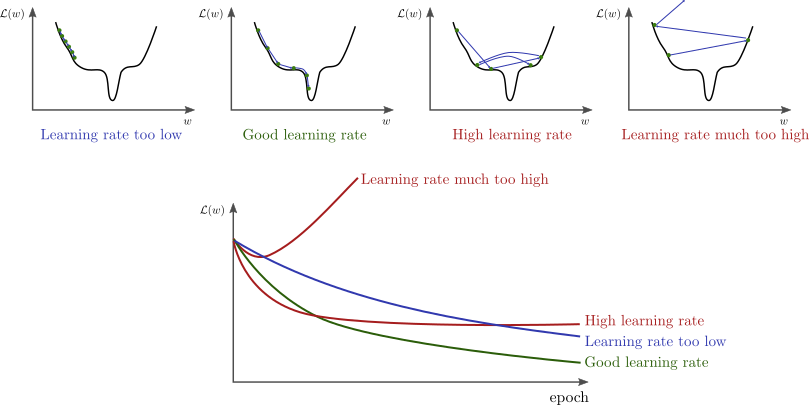
\includegraphics[scale=0.5]{../Figuras/gradiente.png}
 \caption{Rehacerla bien. por copyright..}
 \label{fig:gradiente}
\end{figure}

Lo más habitual es que las capas más alejadas de la salida de la red aprendan más lentamente que las capas más cercanas a la salida. Dado que los niveles de activación de las neuronas están acotados y los resultantados a menudo son menores que 1. En casos extremos, el gradiente será prácticamente nulo, por lo que la red será incapaz de aprender. Dandonos el 
 problema conocido como gradiente desvaneciente en inglés \emph{vanishing gradient}.

 También puede darse el caso opuesto. Si los pesos de la red aumentan en exceso durante el entrenamiento de la red (p.ej. si utilizamos una tasa de aprendizaje demasiado elevada que hace que el gradiente descendente sea inestable y diverja), los factores involucrados en el cálculo del gradiente tomarán valores mucho mayores que 1. En este caso, el problema es el contrario al gradiente devanescente y tendríamos la explosión del gradiente \emph{exploding gradient}.

 \begin{center}
 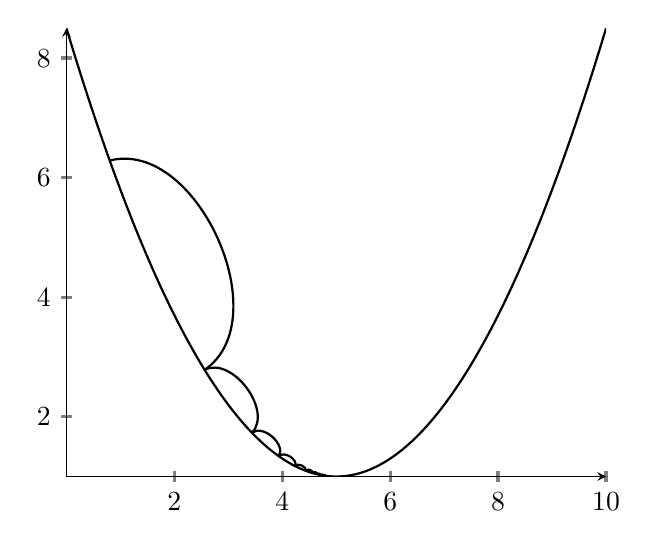
\begin{tikzpicture}
\begin{axis}[
axis lines=middle,
tick style={very thick},
]
%
%line of best fit
\addplot[thick,samples=151,domain=0:10] {0.3*(x-5)^(2) + 1}
foreach \x in {1,...,12} {coordinate[pos={0.5-1.5/pow(1+\x,2)}] (p\x)
\ifnum\x>1
(p\the\numexpr\x-1) edge[bend left=80] (p\x)
\fi};
\end{axis}
\newline
%\caption{Buena taza de aprendizaje. Desenso por el gradiente deseado.}
\end{tikzpicture}
\end{center}

\begin{figure}[H]
 \centering
 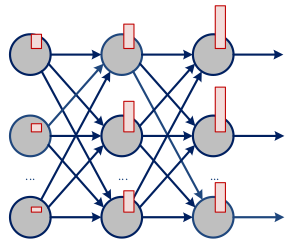
\includegraphics[scale=0.5]{../Figuras/vanish.png}
 \caption{La magnitud del gradiente varía de una capa a otra durante el entrenamiento de una red neuronal multicapa}
 \label{fig:vanish}
\end{figure}

En resumen, el aprendizaje basado en gradiente descendente usando retroporpagación puede no funcionar demasiado bien cuando el nivel de activación de una neurona j es bajo (lo que afecta al ajuste de los pesos de las neuronas que reciben como entrada la salida de la neurona j), las neuronas sigmoidales se estancan (por lo que las derivadas de sus funciones
de activación serán bajas, lo cual afecta al entrenamiento de sus pesos y, potencialmente, al de las neuronas que las preceden en la red) o la profundidad de nuestra red hace que se vea afectada por problemas como desvanecimiento o exploción del gradiente.


\input{secciones/OptimizacionEntrenamiento/03Entrenamiento en línea vs en lotes}
\section{Normalización y normalización por lotes}

Un factor importante a tomar en cuenta para un buen desempeño del entrenamiento son las magnitudes del datos de entrada a la red. Entonces para mejorar el desempeño del algoritmo de optimización nos conviene pre-procesar los datos de entrada. Esto mediante una técnica que se llama normalización (\emph{normalization} en inglés).

La técnica que hemos utilizado son técnicas de optimización basadas en el gradiente, la cual a una función de error se calcula el gradiente, este nos da la dirección del máximo descenso, para  hacer aproximaciones discretas en los parámetros hasta que tratemos de llegar al mínimo de la función.
 
Para poder realizar lo anterior necesitamo que las magnitudes de los datos de entrada no esten muy dispersas, es decir que no nos encontremos con situaciones donde estemos manejando decimales para unos datos y para otros unidades de millones. En estos casos la función de error nunca va a terminar de ajustarse correctamente a estos datos, pues en ocaciónes los parametros para ajustar, van a avanzar de forma distorsionada. Dando la impresión que para unos datos el gradiente avanza muy rapido al centro, mientras que para otros datos avanza muy lento, esto porque vamos a tener curvas de nivel demasiado elípticas (ver la \fref{fig:curvasNivel}), entonces al tomar la dirección que nos de el gradiente, nos va a mover desplazar muy violentamente en algunas y muy lento para otras. Cuando se intente hacer descenso por el gradiente en estas regiones lo que va a pasar es que el vector va a oscilar muy violentamente y  nos va a dificultar mucho llegar al minimo.

Por el contrario, si las magnitudes con las que trabajamos son del mismo orden y contribuyen numéricamente de una manera más proporcionada al error, entonces vamos a tener curvas de nivel  más circulares (ver la \fref{fig:curvasNivel}). Cuando calculemos el gradiente, la perpendicular se aproximará durante más tiempo a la dirección de máximo descenso. 

\begin{figure}[H]
 \centering
 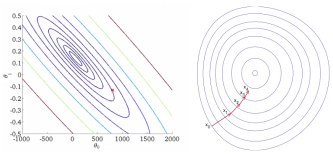
\includegraphics[scale=0.5]{../Figuras/curvasDeNivel.png}
 \caption{Izq: J la función de error con alta excentricidad. Der: J con curvas de nivel tendiendo a círculos}
 \label{fig:curvasNivel}
\end{figure}

Entonces para asegurar un buen desenso por el grandiente, vamos a preferir siempre trabajar con curvas de nivel circulares, para esto vamos a usar la normalización.

La normalización conciste en centrar los datos aproximadamente en el intervalo $[-1.0, 1.0]$, este intervalo no es estricto para todas las redes basta con definir las magnitudes en un intervalo aceptable para tener curvas de nivel circulares. 

Existen varias fórmulas para realizar la normalización, se sugiere la siguiente forma:
\begin{itemize}
 \item Calcular \emph{la media} $\mu_i$ y \emph{varianza} $\sigma_{i}^2$ para cada característica $i$ en los datos del conjunto de entrenamiento $X$.
 \begin{itemize}
  \item Las formulas son las siguientes, con $X_i$ la columna con la i-ésima característica en los datos de entrenamiento $X$.\\
  \begin{equation}
   \mu_{i} = \dfrac{1}{m}\sum_{i=1}^{m}x_{i} 
  \end{equation}
  \begin{equation}
   \sigma_{i}^{2} = \dfrac{1}{m}\sum_{i=1}^{m}(x_{i}-\mu)^2 
  \end{equation}
  \begin{equation}
   X_{i} = \dfrac{X_{i}-\mu}{\sigma^{2}}
  \label{eq:tres}
  \end{equation}
 \end{itemize}
    \item La media es el promedio de los datos de entrada.
    \item La varianza es una medida de dispersión, para ver que tan separados estan los datos unos de otros.
    \item La reasignación para cada $X_i$ va a ser, la resta $X_i -\mu$, que va a centrar los datos alrededor del cero, y la división por la varianza $\sigma^2$ que va a encoger los intervalos de distancia entre los datos. 
\end{itemize}

 
\begin{itemize}
 \item Una vez que la red se entreno con datos normalizados, \textit{es necesario almacenar las medias y varianzas} utilizadas durante el entrenamiento con el conjunto de entrenamiento $X$.
 \item Estos valores serán utilizados para normalizar datos nuevos que vayan a ser evaluados en la red. Esto para evitar que los nuevos datos usen magnitudes fuera del intervalo usado durante el entrenamiento de la red.
\end{itemize}

\begin{definition}
 \emph{La normalización} permite reducir la excentricidad en la función de error provocada por la disparidad entre los datos de entrada.
\end{definition}
  
 Entonces ya tenemos resuelta la situación de la disparides entre los datos de entrada. Ahora tenemos que, al calcular los valores para las capas intermedias, los valores pueden cambiar sus rangos para las neuronas intermedias. Para esta situación tenemos la normalización por lotes (\emph{bach normalization} en inglés).
 
La normalización por lotes aplica los beneficios de la normalización a las capas intermedias, haciendo que estás den valores en intervalos no muy grandes para las siguientes capas.

Una ventaja que nos da esta herramienta es que los algoritmos de optimización podrán utilizar \textit{tazas de aprendizaje más altas}, porque los brincos discretos del algoritmo no cambiarán drásticamente el comportamiento de la función de error durante un intervalo más largo.

Otra ventaja es que al normalizar entre capas, permite que cada capa calcule características distintas, independientemente que se otorguen ejemplares con mucho sesgo en una característica en especial. Permitiendo una mejor clasificación aún con datos nuevos. 

\begin{definition}
 La \emph{normalización por lotes} conciste en: 
 \begin{enumerate}
  \item  Normalizar la salida de la capa de activación anterior restando su media y dividiendo entre la desviación estándar.
  \item Hacer descenso por el gradiente estocástico.
  \item Dos paremetros: $\gamma$ una desviación estandar y $\beta$ una media para corrimiento.
 \end{enumerate}
\end{definition}

Cuando se use el descenso por el gradiente estocástico (el descenso por el gradiente por lotes) modificará los pesos para optimizar $J$ la función de error, y probablemente contrarreste el efecto de la normalización.
Para evitarlo, se añaden dos parámetros, también entrenables: $\gamma$ una desviación estándar y $\beta$ una media para corrimiento, la idea es que el algoritmo tienda a
modificarlos, $\gamma$ para escalarlos y $\beta$ para sesgar los datos, en lugar de a los pesos, de modo que los pesos produzcan un cómputo más estable.

Entonces la idea concreta es que dado un minilote $B$ con $x_i$ sus ejemplares, las entradas $y_i$ para la capa siguiente se
calculan con las siguientes formulas:
  \begin{equation}
   \mu_{B} = \dfrac{1}{m}\sum_{i=1}^{m}x_{i} 
  \end{equation}
  \begin{equation}
   \sigma_{B}^{2} = \dfrac{1}{m}\sum_{i=1}^{m}(x_{i}-\mu_{B})^2 
  \end{equation}
  \begin{equation}
   x_{i} = \dfrac{X_{i}-\mu_{B}}{\sqrt{ \sigma_{B}^{2} + \varepsilon}}
  \label{eq:tres}
  \end{equation}
  \begin{equation}
   y_{i} = \gamma x_{i}+\beta \equiv BN_{\gamma,\beta}(x_{i})
  \label{eq:tres}
  \end{equation}

con $\varepsilon$ una constante agregada para mantener la estabilidad numérica.

Una vez que hayamos hecho la normalización y hecho la reasignación de datos, nos va a dar los nuevos $y_i$'s que van a entrar para participar en la combinación lineal que decide si se activan o no las neuronas de la siguiente capa. Los valores gama y beta nos van a permitir desnormalizar los datos. 

Así llegamos a la parte de \emph{inferencia}, una vez entrenada la red con normalización y normalización por lotes. Vamos a querer usar la red para hacer inferencias, para esto vamos a calcular la media y la varianza sobre los \textit{mini lotes de entrenamiento} la diferencia más grande con respecto a lo  anterior la vamos a tener en el cálculo de la varianza, porque se utiliza la variante sin sesgos, estos valores se van a estimar con los mini lotes del conjunto de entrenamiento y estos van a quedar como \textit{constantes fijas}. Cuando entren los nuevos valores que estamos tratando de evaluar con nuestra red neuronal, ya no vamos a calcular otra vez las $\mu$ y $\sigma$ para las capas intermedias. Sino que vamos a utilizar:

  \begin{equation}
   E[x] = E_{B}[\mu_{B}]
  \end{equation}
  \begin{equation}
   Var[x] = \dfrac{m}{m-1}E_{B}[\sigma_{B}^2] 
  \end{equation}
  

Que son los promedios con los mini lotes que entrenamos, entonces  los valores modificados de los valores de activación de cada capa van a estar dados por:

\begin{equation}
 y = x \dfrac{\gamma}{\sqrt{Var[x]+\varepsilon} } + % \left(\beta-\dfrac{\gammaE[x]}{\sqrt{Var[x] + \varepsilon} } \right)
\end{equation}

Donde $y$ toma el valor $x$ de activación con una red neuronal normal después multiplicarlo por el parámetro gamma (que ya tuvo que haber sido aprendido por el algoritmo de entrenamiento) se va a dividir entre esta desviación estándar pero calculada sobre los datos estadísticos el de lo que salió en esas capas intermedias cuando estábamos realizando el entrenamiento. 

Entonces en resumen la idea es la siguiente, dada  una capa de la red neuronal con sus valores de activación, antes de pasar a la siguiente capa tenemos que pasar por un proceso por un proceso, \textit{la normalización} para ese proceso necesitábamos la media y la varianza. Sin embargo mientras estábamos entrenando esta media y esta varianza podían ser alterados porque estamos modificando los pesos eso modifique los valores que se estaban calculando aquí y por consiguiente  estos dos se van a volver a modificar. Una vez que ese proceso ya terminó y ya decidimos que están fijos los pesos ya tenemos los valores de beta y gamma que vamos a utilizar, es cuando se va a proceder a calcular  la última versión de las medias y las varianzas, con los datos de entrenamiento. 

Cuando tengamos ya estos valores estables porque ya no estamos modificando nada en la red estos los vamos a guardar y se van a convertir en los valores que vamos a utilizar cuando queramos evaluar un dato nuevo sobre la red que ya está entrenada entonces ahora sí cuando llegue a un dato nuevo cada vez que pasemos por alguna de las capas intermedias vamos a tomar esos valores de activación y vamos a aplicar lo equivalente a la fórmula que teníamos antes esta que está aquí nada más que ahora vamos a utilizar estas constantes que se derivan del escalamiento que tuvimos que hacer cuando estábamos entrenando entonces esto que está acá va a ser el valor que va a entrar a la siguiente capa de la red en lugar de haber utilizado el valor de activación como y una vez que hayamos hecho esto entonces nuestra red también va a tener el mismo tipo de normalización para datos que no habían estado en el conjunto de entrenamiento y además pues ésta es normalización es ya no van a estar cambiando porque dependen nada más de los parámetros. 

La mayoría de las apis para el desarrollo de redes neuronales ya tienen estos calculos programados por detrás y nosotros realmente lo único  tenemos que hacer es programarla como una capa, que se le conoce como \textit{capa de normal por lotes}. 

%Para más información también pueden aseguir las siguientes ligas:
%\begin{itemize}
% \item \url{https://www.analyticsvidhya.com/blog/2021/03/introduction-to-batch-normalization/}
% \item \url{https://www.baeldung.com/cs/normalizing-inputs-artificial-neural-network}
% \item \url{https://towardsdatascience.com/why-data-should-be-normalized-before-training-a-neural-network-c626b7f66c7d}
%\end{itemize}


\section{Regularización}

La última técnica a usar en este texto es la técnica de regularización, esta es usada para librarnos de dos problemas al momento de entrenar. Estos problemas son el \textit{sobre ajuste} y el \textit{ajuste pobre}, en inglés \emph{overfitting} y \emph{underfitting} respectivamente.

Recordemos que dado un problema de aprendizaje, se define un espacio de hipótesis, es decir, una familia de posibles funciones que vamos a utilizar para encontrar la función objetivo, que queremos aproximar. 

El espacio de hipótesis puede ser tan grande o tan pequeño como la cantidad de funciones que estén contenidas en él. Así tenemos dos situaciones:
\begin{itemize}
 \item Si el espacio de hipótesis, no contiene a la función objetivo, entonces por más que ejecutemos los algoritmos de entrenamiento, no va a ser posible llegar a una buena aproximación.
 \begin{example}
  Si la función objetivo tiene la forma de una parábola, y únicamente la intentamos aproximar con funciones lineales, es claro que nunca vamos a dar una buena aproximación.
 \end{example}

 \item Si el espacio de hipótesis, es demasiado gigantesco, podemos llegar a tener problemas encontrando la respuesta correcta. 
\end{itemize}

Las dos situaciones anteriores nos llevan a los dos problemas antes mencionados:
\begin{description}
 \item [Ajuste pobre] 
 Cuando un modelo, no logra reducir suficientemente el error sobre el conjunto de entrenamiento (menos aún sobre el de validación) ver \fref{fig:underF}.
  \begin{figure}[H]
   \centering
   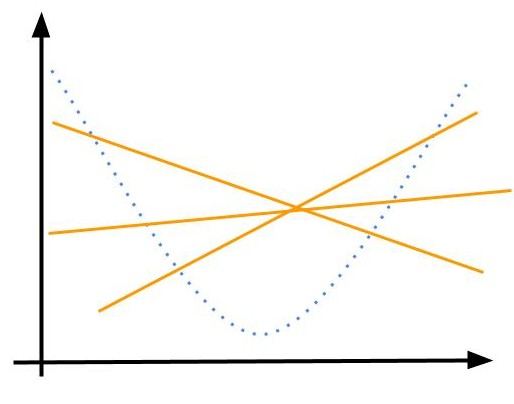
\includegraphics[scale=0.5]{../Figuras/underfitting.jpg}
   \caption{Ejemplo de ajuste pobre. La línea punteada es la función objetivo, las líneas naranjas el espacio de hipótesis.}
   \label{fig:underF}
  \end{figure}

 \item [Sobre ajuste]
 Cuando un modelo, reduce muy bien el error con el conjunto de entrenamiento, pero con el conjunto de validación el error es muy alto, es decir, la hipótesis no generaliza a datos no vistos previamente, ver \fref{fig:overF}.
 \begin{example}
  Los datos del entrenamiento asemejan la función de un polinomio, entonces la red aprende solo a identificar los datos que pasen por la función, al momento de agregar datos nuevos estos probablemente nos se comporten conforme al polinomio y nunca los clasifique adecuadamente. 
 \end{example}

  \begin{figure}[H]
   \centering
   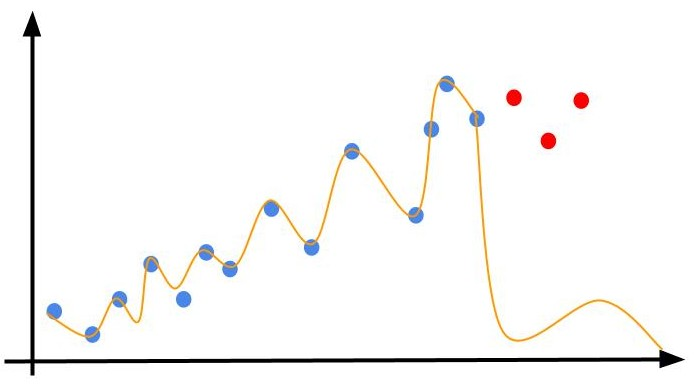
\includegraphics[scale=0.5]{../Figuras/overfitting.jpg}
   \caption{Ejemplo de sobre ajuste. La función aproximada de color naranja. Los datos durante el entrenamiento de color azul. Los datos nuevos de color rojo.}
  \label{fig:overF}
  \end{figure}
 \end{description}

Estos dos problemas puden suceder por dos razones distintas:
\begin{enumerate}
 \item La cantidad de neuronas, dos casos:
    \begin{itemize}
     \item \textbf{Faltan neuronas}: El espacio de hipótesis es muy simple para poder aproximar la función, es decir, tenemos un \textit{ajuste pobre}.
    
    \item \textbf{Sobran neuronas}: El espacio de hipótesis es muy expresivo. No obtiene las características de la función objetivo, sino que memorizó las etiquetas de los datos de entrada, es decir, tenemos un \textit{sobreajuste}.
    \end{itemize}

 \item Faltan datos de entrenamiento, entonces independientemente del número de neuronas, el error en los datos de validación no baja, o incluso ni en los datos del entrenamiento.
\end{enumerate}

Cuando nos sobran nueronas lo podemos detectar, porque al reducir neuronas, el desempeño de la red entrenada en el conjunto de entrenamineto, no empeora significativamente, y el desempeño con los datos de validación mejora.

Para automatizar la búsqueda en un espacio de hipótesis lo suficientemente expresiva vamos a usar la regularización.

Lo que vamos a hacer es modificar la función de pérdida, la nueva función va a estar integrada por dos componentes; la función de error (que ya teníamos), y un  término de penalización sobre las magnitudes de los pesos de la red. Considerando estas dos anteriores,  la función que estamos tratando de minimizar es  la suma de esas dos.

El mínimo de esta función hallará un punto de compromiso tal que:
\begin{itemize}
 \item reduce el error lo más posible
 \item solo crecen aquellos pesos que contribuyen mejor a reducir el error, compensando por la contribución de su magnitud creciente.
\end{itemize}

Es decir ahora tenemos una red en la cual colocamos desde el inicio muchas neuronas, lo cual tendería a producir un sobre ajuste. Lo que vamos a hacer es, penalizar los pesos de manera que el algoritmo de optimización haga que solamente aquellas conexiones que realmente están contribuyendo a reducir el error, tengan magnitudes significativas. Aquellas conexiones que no contribuyan entenderán a tener magnitudes muy pequeñas, casi como si no estuvieran ahí. El algoritmo de optimización hara que algunas de las conexiones queden muy débiles y básicamente ya no contribuyan. Entonces la hipótesis que se va a aprender va a ser más sencilla.

Dependiendo de qué tan rigurosos seamos con la penalización podemos hacer que, las únicas conexiones que pueden subir su magnitud en realidad sean muy pocas. También podría darse el problema de ajuste pobre, se  tiene que ajustar bien el termino de penalización que lo vamos a denotar como \emph{$\lambda$}.

La función de perdida se va actualizar de la siguiente forma:
\begin{equation}
 J(\Theta) = Error(\Theta)+\dfrac{\lambda}{2m}\sum_{\Theta}\theta^2
 \label{eq:errorR}
\end{equation}

\begin{equation}
 \nabla_{\theta}J^{(l)} = \nabla Error_{\Theta}^{(l)}+\dfrac{\lambda}{m}\left[ \right]
\end{equation}
%\begin{bmatrix} 0 \\ \Theta_{[:,1:]} \end{bmatrix}

Entonces vamos a tener una gráfica parecida a la siguiente:
  \begin{figure}[H]
   \centering
   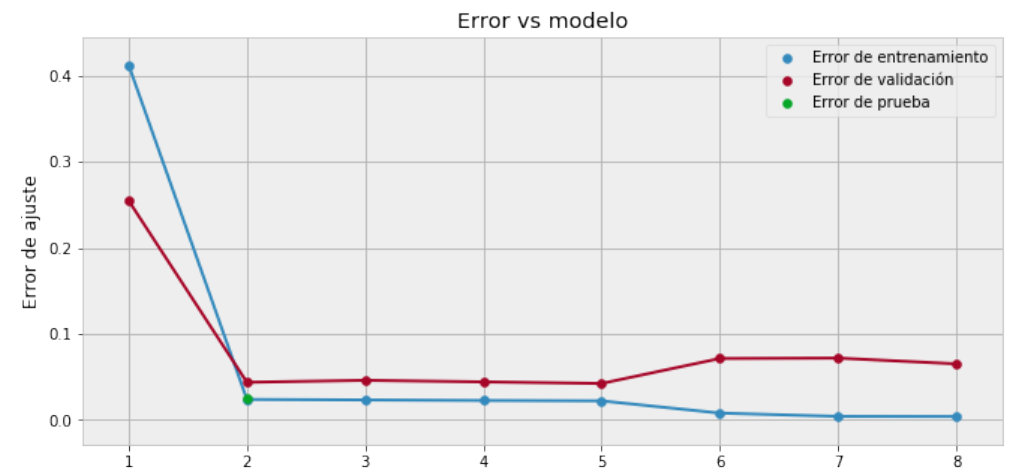
\includegraphics[width=\textwidth ]{../Figuras/graficaOO.png}
   \caption{Sobreajuste.}
  \label{fig:grafica00}
  \end{figure}

 En la ecuación \ref{eq:errorR} que del lado izquierdo tenemos nuestra función de error (podría ser una entropía cruzada, diferencias cuadrado), el segundo término es la penalización, la más común es  sumar los todos los cuadrados de las magnitudes, de todos los pesos que tienen la red, este término va a provocar que la función suba de valor, si estamos utilizando pesos con magnitudes grandes. 
 
 La manera de minimizar los valores, es dejar subir solamente los valores de aquellos pesos que ayuden a compensar, bajando la penalización. La penalización está regida por el parámetro lambda, entre más grande sea lambda, se observa en la \fref{fig:grafica00} que se incrementa el valor de esta función, por culpa de los pesos. Entonces, si la lambda es muy pequeña el término dominante va a ser la función original de error y poca penalización por tanto muy poco efecto, por el hecho de haberle subido la magnitud de los pesos, vamos a obtener un sobreajuste. Esto equivaldría a tener nuestra red neuronal con el montón de neuronas que le pusimos, no hay penalización y podríamos tender precisamente al problema del sobreajuste. 
 
 Entonces vaemos el lado derecho de la gráfica \fref{fig:grafica00}. El error en el entrenamiento se esta penalizando tanto por los pesos que el algoritmo de optimización, minimizo los pesos y casi no corregio el error, entonces tenemos un ajuste pobre. En ese caso  nuestra red  no está modelando bien nuestra función, tenemos un error bastante alto y la función de validación también está creciendo. 
 
 En el la parte de en medio de la gráfica \fref{fig:grafica00} es donde de obtiene el equilibrio, entre la cantidad de neuronas adecudas y la cantidad de pesos significativos, que nos va a minimizar o eliminar el problema de un pobre o un sobre ajuste.
 
 \subsection{Dropout}
 
 Otra estrategia para regularizar es la deserción o descarte de algunas neuronas(\emph{dropout} en inglés). 
 Durante el entrenamiento, una cierta cantidad de salidas de capas ocultas se ignoran \emph{aleatoriamente} (se les da valor final de 0) con probabilidad $1-p$, es decir algunas neuronas de las capas ocultas se activan con un probablidad $p$. 

 En esta técnica no se modifica la función de error, si no se modifica propiamente la red, ver \fref{fig:dropout}. En cada epoca, durante el entrenamiento se puede volver a elegir las neuronas a descartar, o no. 
 La capa alterará su conectividad y buscará caminos alternativos para transmitir la información en la siguiente capa. Como resultado, cada actualización de una capa durante el entrenamiento se realiza con una configuración diferente de la capa. Así se puede simular el entrenamiento de una gran cantidad de redes neuronales con diferentes arquitecturas en paralelo.

  \begin{figure}[h]
   \centering
   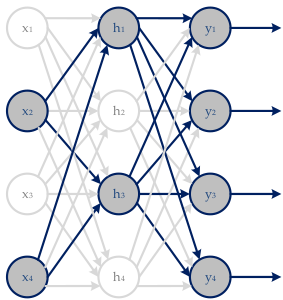
\includegraphics[scale=.5]{../Figuras/dropout.png}
   \caption{Dropout (desarrollado por Geoffrey Hinton y sus estudiantes en la Universidad de Toronto).}
  \label{fig:dropout}
  \end{figure}

 Al momento de pasar los datos de prueba, todas las neuronas están activas. Pero se han reducido en p, esto sucede porque después de la eliminación en el entrenamiento, las siguientes capas recibirán valores más bajos. Sin embargo, en la fase de prueba, mantendremos todas las unidades, por lo que los valores serán mucho más altos de lo esperado, es por eso que necesitamos reducirlos, por un facto igual a la tasa de deserción p, para equilibrar el hecho de que hay más unidades activas que en tiempo de entrenamiento. Para información del tema puede leer el capítulo cuatro, sección 4.4.3 Adding dropout, Deep Learning With Python, 2017.  
 
 



\chapter{Caso de análisis e interpretación}
\input{secciones/CasoAnalisisInterpretacion/01Red Hinton árbol familiar con numpy (entrenamiento)}
\input{secciones/CasoAnalisisInterpretacion/02Red Hinton árbol familiar con pytorch}

\chapter{Entrenamiento con genéticos}
%\section{MNIST versión básica con numpy}
\input{secciones/EntrenamientoGeneticos/01Algoritmos genéticos}
\input{secciones/EntrenamientoGeneticos/02Neuroevolución}
\subsection{Antecedentes: Aprendizaje por refuerzo en videojuegos}
Vacio.

\input{secciones/EntrenamientoGeneticos/022Arquitectura para estimar la función de recompensa}
\subsection{Entrenamiento}
Vacio.


%\part{Aprendizaje no supervisado}
\chapter{Mapeos autoorganizados}
\input{secciones/cap10/00Introducción}
\section{Aprendizaje no supervisado}
Vacio.

\section{Mapeos autoo-organizados}
Vacio.

\section{Kohonen}
Vacio.


%%
%\part{NO TIENE NOMBRE}
\chapter{Redes Neuronales Convolucionales}
\section{Convolución}
\section{Redes Convolucionales}
\section{Softmax}
\section{MNIST}

%%
\part{Redes con ciclos}
\chapter{Redes Neuronales Recurrentes}
\section{Derivadas ordenadas}
\section{Retropropagación en el tiempo}
\section{Sistemas dinámicos y despliegue del grafo}
\section{Arquitectura recurrente universal}
\section{Función de error}
\section{Forzamiento del profesor}

\chapter{Atención}
%\section{Casos de análisis de serie}
\chapter{LSTM}
\chapter{GRU}
\chapter{Casos de análisis: etiquetado de palabras y conjugación de verbos}

\part{Redes no dirigidas}
\chapter{Redes de hopfield}
\section{Entrenamiento}

\chapter{Máquinas de Boltzman}
\section{Entrenamiento}
\subsection{Partículas y partículas de fantasía}
\subsection{Máquinas de Boltzman Restringidas}

\chapter{Redes adversarias}
\section{GANs}

\appendix 
\chapter{Ecuaciones diferenciales}

%----------------------------------------------------------------------------------------
% Bibliografia
%----------------------------------------------------------------------------------------
\backmatter

\printbibliography[heading=bibintoc]

\end{document}
